% !TeX encoding = UTF-8
% !TeX program = xelatex
% !TeX spellcheck = en_US

\documentclass[degree=master]{thuthesis}
  % 学位 degree:
  %   doctor | master | bachelor | postdoc
  % 学位类型 degree-type:
  %   academic(默认)| professional
  % 语言 language
  %   chinese(默认)| english
  % 字体库 fontset
  %   windows | mac | fandol | ubuntu
  % 建议终版使用 Windows 平台的字体编译


% 论文基本配置,加载宏包等全局配置
% !TeX root = ./thuthesis-example.tex

% 论文基本信息配置

\thusetup{
  %******************************
  % 注意:
  %   1. 配置里面不要出现空行
  %   2. 不需要的配置信息可以删除
  %   3. 建议先阅读文档中所有关于选项的说明
  %******************************
  %
  % 输出格式
  %   选择打印版(print)或用于提交的电子版(electronic),前者会插入空白页以便直接双面打印
  %
  output = print,
  %
  % 标题
  %   可使用“\\”命令手动控制换行
  %
  title  = {清华大学学位论文 \LaTeX{} 模板\\使用示例文档 v\version},
  title* = {An Introduction to \LaTeX{} Thesis Template of Tsinghua
            University v\version},
  %
  % 学位
  %   1. 学术型
  %      - 中文
  %        需注明所属的学科门类,例如:
  %        哲学、经济学、法学、教育学、文学、历史学、理学、工学、农学、医学、
  %        军事学、管理学、艺术学
  %      - 英文
  %        博士:Doctor of Philosophy
  %        硕士:
  %          哲学、文学、历史学、法学、教育学、艺术学门类,公共管理学科
  %          填写“Master of Arts“,其它填写“Master of Science”
  %   2. 专业型
  %      直接填写专业学位的名称,例如:
  %      教育博士、工程硕士等
  %      Doctor of Education, Master of Engineering
  %   3. 本科生不需要填写
  %
  degree-name  = {工学硕士},
  degree-name* = {Master of Science},
  %
  % 培养单位
  %   填写所属院系的全名
  %
  department = {计算机科学与技术系},
  %
  % 学科
  %   1. 学术型学位
  %      获得一级学科授权的学科填写一级学科名称,其他填写二级学科名称
  %   2. 工程硕士
  %      工程领域名称
  %   3. 其他专业型学位
  %      不填写此项
  %   4. 本科生填写专业名称,第二学位论文需标注“(第二学位)”
  %
  discipline  = {计算机科学与技术},
  discipline* = {Computer Science and Technology},
  %
  % 姓名
  %
  author  = {薛瑞尼},
  author* = {Xue Ruini},
  %
  % 指导教师
  %   中文姓名和职称之间以英文逗号“,”分开,下同
  %
  supervisor  = {郑纬民, 教授},
  supervisor* = {Professor Zheng Weimin},
  %
  % 副指导教师
  %
  associate-supervisor  = {陈文光, 教授},
  associate-supervisor* = {Professor Chen Wenguang},
  %
  % 联合指导教师
  %
  % co-supervisor  = {某某某, 教授},
  % co-supervisor* = {Professor Mou Moumou},
  %
  % 日期
  %   使用 ISO 格式;默认为当前时间
  %
  % date = {2019-07-07},
  %
  % 是否在中文封面后的空白页生成书脊(默认 false)
  %
  include-spine = false,
  %
  % 密级和年限
  %   秘密, 机密, 绝密
  %
  % secret-level = {秘密},
  % secret-year  = {10},
  %
  % 博士后专有部分
  %
  % clc                = {分类号},
  % udc                = {UDC},
  % id                 = {编号},
  % discipline-level-1 = {计算机科学与技术},  % 流动站(一级学科)名称
  % discipline-level-2 = {系统结构},          % 专业(二级学科)名称
  % start-date         = {2011-07-01},        % 研究工作起始时间
}

% 载入所需的宏包

% 定理类环境宏包
\usepackage{amsthm}
% 也可以使用 ntheorem
% \usepackage[amsmath,thmmarks,hyperref]{ntheorem}

\thusetup{
  %
  % 数学字体
  % math-style = GB,  % GB | ISO | TeX
  math-font  = xits,  % sitx | xits | libertinus
}

% 可以使用 nomencl 生成符号和缩略语说明
% \usepackage{nomencl}
% \makenomenclature

% 表格加脚注
\usepackage{threeparttable}

% 表格中支持跨行
\usepackage{multirow}

% 固定宽度的表格。
% \usepackage{tabularx}

% 跨页表格
\usepackage{longtable}

% 算法
\usepackage{algorithm}
\usepackage{algorithmic}

% 量和单位
\usepackage{siunitx}

% 参考文献使用 BibTeX + natbib 宏包
% 顺序编码制
\usepackage[sort]{natbib}
\bibliographystyle{thuthesis-numeric}

% 著者-出版年制
% \usepackage{natbib}
% \bibliographystyle{thuthesis-author-year}

% 本科生参考文献的著录格式
% \usepackage[sort]{natbib}
% \bibliographystyle{thuthesis-bachelor}

% 参考文献使用 BibLaTeX 宏包
% \usepackage[backend=biber,style=thuthesis-numeric]{biblatex}
% \usepackage[backend=biber,style=thuthesis-author-year]{biblatex}
% \usepackage[backend=biber,style=apa]{biblatex}
% \usepackage[backend=biber,style=mla-new]{biblatex}
% 声明 BibLaTeX 的数据库
% \addbibresource{ref/refs.bib}

% 定义所有的图片文件在 figures 子目录下
\graphicspath{{figures/}}

% 数学命令
\makeatletter
\newcommand\dif{%  % 微分符号
  \mathop{}\!%
  \ifthu@math@style@TeX
    d%
  \else
    \mathrm{d}%
  \fi
}
\makeatother

% hyperref 宏包在最后调用
\usepackage{hyperref}



\begin{document}

% 封面
\maketitle

% 学位论文指导小组、公开评阅人和答辩委员会名单
% 本科生不需要
% % !TeX root = ../thuthesis-example.tex

\begin{committee}[name={学位论文指导小组、公开评阅人和答辩委员会名单}]

  \newcolumntype{C}[1]{@{}>{\centering\arraybackslash}p{#1}}

  \section*{指导小组名单}

  \begin{center}
    \begin{tabular}{C{3cm}C{3cm}C{9cm}@{}}
      李XX & 教授     & 清华大学 \\
      王XX & 副教授   & 清华大学 \\
      张XX & 助理教授 & 清华大学 \\
    \end{tabular}
  \end{center}


  \section*{公开评阅人名单}

  \begin{center}
    \begin{tabular}{C{3cm}C{3cm}C{9cm}@{}}
      刘XX & 教授   & 清华大学                    \\
      陈XX & 副教授 & XXXX大学                    \\
      杨XX & 研究员 & 中国XXXX科学院XXXXXXX研究所 \\
    \end{tabular}
  \end{center}


  \section*{答辩委员会名单}

  \begin{center}
    \begin{tabular}{C{2.75cm}C{2.98cm}C{4.63cm}C{4.63cm}@{}}
      主席 & 赵XX                  & 教授                    & 清华大学       \\
      委员 & 刘XX                  & 教授                    & 清华大学       \\
          & \multirow{2}{*}{杨XX} & \multirow{2}{*}{研究员} & 中国XXXX科学院 \\
          &                       &                         & XXXXXXX研究所  \\
          & 黄XX                  & 教授                    & XXXX大学       \\
          & 周XX                  & 副教授                  & XXXX大学       \\
      秘书 & 吴XX                  & 助理研究员              & 清华大学       \\
    \end{tabular}
  \end{center}

\end{committee}



% 也可以导入 Word 版转的 PDF 文件
% \begin{committee}[file=figures/committee.pdf]
% \end{committee}


% 使用授权的说明
\copyrightpage
% 将签字扫描后授权文件 scan-copyright.pdf 替换原始页面
% \copyrightpage[file=scan-copyright.pdf]

\frontmatter
% !TeX root = ../thuthesis-example.tex

% 中英文摘要和关键字

\begin{abstract}
随着自动驾驶技术的日渐成熟,自动驾驶车辆和人工驾驶车辆混行很有可能成为未来道路上的常见场景。
在本课题中,首先为自动驾驶和人工驾驶车辆选择了合适的跟驰模型,并对混合车队的队列稳定性进行了分析,
接着通过数值仿真的方法,探究了混合车队的队列稳定性与碰撞风险之间的关系,同时探讨了碰撞风险在混合车队中的演化机理。

本工作的意义在于,碰撞风险评价指标的获得往往滞后于危险的发生,这不利于交通事故的预测与防范。如果能建立混合车队
队列稳定性与碰撞风险的关系,就可以通过队列的稳定性对车队的碰撞风险进行评估,起到预防交通事故的作用。同时,通过对碰撞风险
演化机理的探究,发现混合车队的排列情况也会影响车队的碰撞风险,其中的机理和规律可以指导车队选择碰撞风险更小的排列方式。


  % 关键词用“英文逗号”分隔,输出时会自动处理为正确的分隔符
  \thusetup{
    keywords = {自动驾驶, 混合车队, 队列稳定性, 碰撞风险},
  }
\end{abstract}

\begin{abstract*}
  
With the development of autonomous driving technology, 
the mixed driving of autonomous vehicles and human-driven vehicles is likely to become a common situation in the future.
In this study, the appropriate car-following models are firstly selected for autonomous and human-driven vehicles,
and the string stability of the mixed vehicular platoon is analyzed.
Besides, the relationship between the string stability and the crash risk, 
as well as the evolution mechanism of the crash risk,  of the mixed vehicular platoon is discussed 
through the situation. 

The significance of this work is that the acquisition of the evaluation of crash risk usually lags behind the
occurrence of danger, which is not conducive to the prediction and prevention of traffic accidents.
Once we build the relationship between the string stability and the crash risk of the mixed vehicular platoon,
we can use the former to predict the latter,
which plays a role in preventing traffic accidents. 
At the same time, the arrangement of the mixed vehicular platoon also affects the crash risk,
and it is significant to study the evolution mechanism of the crash risk 
to guide the mixed vehicular platoon to choose the arrangement with less crash risk.

  % Use comma as separator when inputting
  \thusetup{
    keywords* = {automated vehicles, mixed vehicular platoon, string stability, crash risk},
  }
\end{abstract*}

% 目录
\tableofcontents

% 插图和附表清单
% 本科生的插图索引和表格索引需要移至正文之后、参考文献前
% \listoffiguresandtables  % 插图和附表清单(仅限研究生)
\listoffigures           % 插图清单
\listoftables            % 附表清单

% 符号对照表
% !TeX root = ../thuthesis-example.tex

\begin{denotation}[3cm]
  \item[PI] 聚酰亚胺
  \item[MPI] 聚酰亚胺模型化合物,N-苯基邻苯酰亚胺
  \item[PBI] 聚苯并咪唑
  \item[MPBI] 聚苯并咪唑模型化合物,N-苯基苯并咪唑
  \item[PY] 聚吡咙
  \item[PMDA-BDA] 均苯四酸二酐与联苯四胺合成的聚吡咙薄膜
  \item[MPY] 聚吡咙模型化合物
  \item[As-PPT] 聚苯基不对称三嗪
  \item[MAsPPT] 聚苯基不对称三嗪单模型化合物,3,5,6-三苯基-1,2,4-三嗪
  \item[DMAsPPT] 聚苯基不对称三嗪双模型化合物(水解实验模型化合物)
  \item[S-PPT] 聚苯基对称三嗪
  \item[MSPPT] 聚苯基对称三嗪模型化合物,2,4,6-三苯基-1,3,5-三嗪
  \item[PPQ] 聚苯基喹噁啉
  \item[MPPQ] 聚苯基喹噁啉模型化合物,3,4-二苯基苯并二嗪
  \item[HMPI] 聚酰亚胺模型化合物的质子化产物
  \item[HMPY] 聚吡咙模型化合物的质子化产物
  \item[HMPBI] 聚苯并咪唑模型化合物的质子化产物
  \item[HMAsPPT] 聚苯基不对称三嗪模型化合物的质子化产物
  \item[HMSPPT] 聚苯基对称三嗪模型化合物的质子化产物
  \item[HMPPQ] 聚苯基喹噁啉模型化合物的质子化产物
  \item[PDT] 热分解温度
  \item[HPLC] 高效液相色谱(High Performance Liquid Chromatography)
  \item[HPCE] 高效毛细管电泳色谱(High Performance Capillary lectrophoresis)
  \item[LC-MS] 液相色谱-质谱联用(Liquid chromatography-Mass Spectrum)
  \item[TIC] 总离子浓度(Total Ion Content)
  \item[\textit{ab initio}] 基于第一原理的量子化学计算方法,常称从头算法
  \item[DFT] 密度泛函理论(Density Functional Theory)
  \item[$E_a$] 化学反应的活化能(Activation Energy)
  \item[ZPE] 零点振动能(Zero Vibration Energy)
  \item[PES] 势能面(Potential Energy Surface)
  \item[TS] 过渡态(Transition State)
  \item[TST] 过渡态理论(Transition State Theory)
  \item[$\increment G^\neq$] 活化自由能(Activation Free Energy)
  \item[$\kappa$] 传输系数(Transmission Coefficient)
  \item[IRC] 内禀反应坐标(Intrinsic Reaction Coordinates)
  \item[$\nu_i$] 虚频(Imaginary Frequency)
  \item[ONIOM] 分层算法(Our own N-layered Integrated molecular Orbital and molecular Mechanics)
  \item[SCF] 自洽场(Self-Consistent Field)
  \item[SCRF] 自洽反应场(Self-Consistent Reaction Field)
\end{denotation}



% 也可以使用 nomencl 宏包,需要在导言区
% \usepackage{nomencl}
% \makenomenclature

% 在这里输出符号说明
% \printnomenclature[3cm]

% 在正文中的任意为都可以标题
% \nomenclature{PI}{聚酰亚胺}
% \nomenclature{MPI}{聚酰亚胺模型化合物,N-苯基邻苯酰亚胺}
% \nomenclature{PBI}{聚苯并咪唑}
% \nomenclature{MPBI}{聚苯并咪唑模型化合物,N-苯基苯并咪唑}
% \nomenclature{PY}{聚吡咙}
% \nomenclature{PMDA-BDA}{均苯四酸二酐与联苯四胺合成的聚吡咙薄膜}
% \nomenclature{MPY}{聚吡咙模型化合物}
% \nomenclature{As-PPT}{聚苯基不对称三嗪}
% \nomenclature{MAsPPT}{聚苯基不对称三嗪单模型化合物,3,5,6-三苯基-1,2,4-三嗪}
% \nomenclature{DMAsPPT}{聚苯基不对称三嗪双模型化合物(水解实验模型化合物)}
% \nomenclature{S-PPT}{聚苯基对称三嗪}
% \nomenclature{MSPPT}{聚苯基对称三嗪模型化合物,2,4,6-三苯基-1,3,5-三嗪}
% \nomenclature{PPQ}{聚苯基喹噁啉}
% \nomenclature{MPPQ}{聚苯基喹噁啉模型化合物,3,4-二苯基苯并二嗪}
% \nomenclature{HMPI}{聚酰亚胺模型化合物的质子化产物}
% \nomenclature{HMPY}{聚吡咙模型化合物的质子化产物}
% \nomenclature{HMPBI}{聚苯并咪唑模型化合物的质子化产物}
% \nomenclature{HMAsPPT}{聚苯基不对称三嗪模型化合物的质子化产物}
% \nomenclature{HMSPPT}{聚苯基对称三嗪模型化合物的质子化产物}
% \nomenclature{HMPPQ}{聚苯基喹噁啉模型化合物的质子化产物}
% \nomenclature{PDT}{热分解温度}
% \nomenclature{HPLC}{高效液相色谱(High Performance Liquid Chromatography)}
% \nomenclature{HPCE}{高效毛细管电泳色谱(High Performance Capillary lectrophoresis)}
% \nomenclature{LC-MS}{液相色谱-质谱联用(Liquid chromatography-Mass Spectrum)}
% \nomenclature{TIC}{总离子浓度(Total Ion Content)}
% \nomenclature{\textit{ab initio}}{基于第一原理的量子化学计算方法,常称从头算法}
% \nomenclature{DFT}{密度泛函理论(Density Functional Theory)}
% \nomenclature{$E_a$}{化学反应的活化能(Activation Energy)}
% \nomenclature{ZPE}{零点振动能(Zero Vibration Energy)}
% \nomenclature{PES}{势能面(Potential Energy Surface)}
% \nomenclature{TS}{过渡态(Transition State)}
% \nomenclature{TST}{过渡态理论(Transition State Theory)}
% \nomenclature{$\increment G^\neq$}{活化自由能(Activation Free Energy)}
% \nomenclature{$\kappa$}{传输系数(Transmission Coefficient)}
% \nomenclature{IRC}{内禀反应坐标(Intrinsic Reaction Coordinates)}
% \nomenclature{$\nu_i$}{虚频(Imaginary Frequency)}
% \nomenclature{ONIOM}{分层算法(Our own N-layered Integrated molecular Orbital and molecular Mechanics)}
% \nomenclature{SCF}{自洽场(Self-Consistent Field)}
% \nomenclature{SCRF}{自洽反应场(Self-Consistent Reaction Field)}



% 正文部分
\mainmatter
% !TeX root = ../thuthesis-example.tex

\chapter{引言}

\section{研究背景}

根据世界卫生组织(WHO)2018年发布的《2018年全球道路安全现状报告》,全球每年交通事故死亡人数达到了135万。交通事故已经成为5至29岁人群的主要死亡原因。对于发展中国家,
道路交通安全形势更加严峻。\cite{WHO} 根据国家统计局发布的数据,2022年我国共发生交通事故2.4万余起,交通事故死亡人数总计6.1万余人,交通事故造成直接财产损失13余
亿元。\cite{stats_gov}

随着科学技术的发展,自动驾驶技术日渐成熟,各大国内外公司和研究机构都表现出了对自动驾驶技术的浓厚兴趣。自动驾驶技术有望减轻驾驶员的驾驶负担、为残障人士和老人提供自动
驾驶服务、提高道路交通安全、改善道路拥挤堵塞情况,并很可能在不远的未来成为影响交通状况、交通安全的重要元素。但自动驾驶汽车的加入,也会引入新的问题,一方面,
随着自动驾驶技术的逐渐普及,可以预见将长期存在自动驾驶车辆和人工驾驶车辆共存的局面,这会使得交通路况更加复杂,引入更多的不确定性因素和安全隐患;
另一方面,目前自动驾驶技术和测试手段仍然不够成熟,自动驾驶相关法律仍在完善之中,法律责任的确定比较模糊,这些问题使得人们仍然对自动驾驶心存顾虑。

近年来,美国电动汽车及能源公司特斯拉因为自动驾驶技术已发生多起安全事故。2018年5月8日,在美国佛罗里达州劳德代尔堡,一辆2014年产的特斯拉汽车撞上混泥土墙并起火,造成
2名高中生死亡,另有一名高中人受伤;2021年5月7日,在中国广东省韶关市,一辆特斯拉汽车追尾一辆小型货车,造成前者驾驶人当场死亡。这些事故使得人们越来越关注自动驾驶的安全问题。

车队的控制有一个特殊的困难,称为“队列不稳定性”,即系统中的扰动沿着车队不断放大。自动驾驶技术的引入,使得人类可以更加精准地控制车辆,通过控制手段,可以使车队达到“稳定”。
围绕车队稳定性,已经有非常丰富的研究。

碰撞风险评价指标的获得往往是滞后于潜在危险发生的,这不利于交通危险的预测与防范。直观感受上,车队中车辆在速度和位置上的波动是造成车辆碰撞的主要原因,前者可以用车队的队列稳定性来描述,后者可以用碰撞风险来描述,如果能将二者建立联系,就能够用车队的队列稳定性
预测碰撞风险,同时可以通过控制车队的队列稳定程度达到减小碰撞概率的目的,提高道路交通安全程度。

本研究旨在建立自动驾驶车辆和人工驾驶车辆混合车队情景下队列稳定性与碰撞风险的关系,探究碰撞风险在车队中的演化机理,为车队的安全性分析提供理论基础。




\section{国内外研究现状综述}

\subsection{跟驰行为建模研究现状}

驾驶员的驾驶行为和所产生的车辆运行特征是研究交通流的基础。而非自由驾驶情况下,车辆直接的相互作用和导致的交通流变化则是研究的重点。

车辆运动行为主要可以分为车辆跟驰行为和换道行为两大类,跟驰模型的研究对象是前者。用数学模式对跟驰行为加以分析阐明,使得研究人员可以定量地描述跟驰行为,对现代交通的模拟有着重要的意义。
跟驰模型研究主要是运用动力学、统计学等方法,利用驾驶行为问卷调查、模拟驾驶或自然驾驶实验的方式,对前车速度、加速度等行车特征变化引起后车的反应进行研究。

研究者提出了多种跟驰模型,下面分别进行简要介绍。 \\

\noindent \textbf{(1)刺激-反应跟驰模型}

刺激-反应跟驰模型最早由Reuschel\cite{reuschel1950vehicle}和Pipes\cite{Pipes}分别单独提出,其假定驾驶员试图调节车辆速度与前车速度保持一致。

假定驾驶员存在反应延迟,可以得到如下的车辆行驶动力学方程:

\begin{equation}
  a_n(t+T) = c\increment{v_{n, n-1}}(t)
  \label{eq:chap01-1}
\end{equation}
其中,

\begin{table}
  \centering
  \caption{刺激-反应跟驰模型符号说明}
  \begin{tabular}{cc}
    \toprule
    符号          &  含义                         \\
    \midrule
    $a_n(t)$   & 第$n$辆车在$t$时刻的加速度         \\
    $v_n(t)$   & 第$n$辆车在$t$时刻的速度         \\
    $c$        & 待定比例系数                    \\
    $T$        & 驾驶员的反应延迟时间 \\
    $\increment{v_{n, n-1}}(t)$  &  第$n$辆车与其前车(第$n-1$辆车)在$t$时刻的速度差   \\
    \bottomrule
  \end{tabular}
  \label{tab:chap01-1}
\end{table}

该模型建立了两个被后续研究公认的基础假设:一是驾驶员将考虑本车和前车的速度差来调节车速;二是驾驶员存在反应延迟。但该模型较为简单,不能较好地
符合实际测得的驾驶员加速度特征。Denos C. Gazis等人将自车速度及其前后车距引入刺激-反应跟驰模型,得到了著名的GHR模型\cite{Gazis1961NonlinearFM}:

\begin{equation}
  a_n(t+T) = cv_n^m(t)\frac{\increment{v_{n, n-1}}(t)}{\increment{x_{n, n-1}^l}(t)}
  \label{eq:chap01-2}
\end{equation}
其中,各符号含义在表\ref{tab:chap01-2}中给出。

\begin{table}
  \centering
  \caption{GHR跟驰模型符号说明}
  \begin{tabular}{cc}
    \toprule
    符号          &  含义                         \\
    \midrule
    $a_n(t)$   & 第$n$辆车在$t$时刻的加速度         \\
    $v_n(t)$   & 第$n$辆车在$t$时刻的速度         \\
    $c$        & 待定比例系数                    \\
    $T$        & 驾驶员的反应延迟时间  \\
    $m, l$        & 幂次系数         \\
    $\increment{v_{n, n-1}}(t)$  &  第$n$辆车与其前车(第$n-1$辆车)在$t$时刻的速度差   \\
    $\increment{x_{n, n-1}}(t)$  &  第$n$辆车与其前车(第$n-1$辆车)在$t$时刻的距离   \\
    \bottomrule
  \end{tabular}
  \label{tab:chap01-2}
\end{table}

GHR模型引入了更多参数,表\ref{tab:chap01-3}列出了一些学者的模型拟合结果:

\begin{longtable}{ccc}
  \caption{部分文献中的GHR模型$m$和$l$的取值} \\
  \toprule
  模型出处 & $m$ & $l$ \\
  \midrule
\endfirsthead
  \caption[]{部分文献中的GHR模型$m$和$l$的取值(续)} \\
  \toprule
  模型出处 & $m$ & $l$ \\
  \midrule
\endhead
  \bottomrule
\endfoot
Chandler et al. (1958)      \cite{1958Traffic}         &   0      &   0      \\
\hline
Herman and Potts (1959)      \cite{herman1959single}   &   0      &   1      \\
\hline
Helly (1959)                 \cite{helly1959simulation}&   1      &   1      \\
\hline
Gazis et al. (1961)          \cite{gazis1961nonlinear} & $0-2$    & $1-2$    \\
\hline
May and Keller (1967)        \cite{may1967non}         & 0.8      &  2.8     \\
\hline
Heyes and Ashworth (1972)    \cite{heyes1972further}   & -0.8     &  1.2     \\
\hline
\multirow{3}*{Hoefs (1972)   \cite{hoefs1972entwicklung}} & 减速:1.5 & 减速:0.9 \\
                                                       & 刹车:0.2 & 刹车:0.9 \\
                                                       & 加速:0.6 & 加速:3.2 \\
Ceder and May (1976)         \cite{ceder1976further}   &   0.6    &   2.4    \\
\hline
\multirow{3}*{Aron (1988)    \cite{aron1988car}}       & 减速:2.5 & 减速:0.7 \\
                                                       & 平稳:2.7 & 平稳:0.3 \\
                                                       & 加速:2.5 & 加速:0.1 \\
\hline
\multirow{2}*{Ozaki (1993)   \cite{ozaki1993reaction}} & 减速:0.9 & 减速:1 \\
                                                       & 加速:-0.2& 加速:0.2            
  \label{tab:chap01-3}
\end{longtable}

因为不同的研究者来自不同的地区,不同地区的驾驶员有着不同的驾驶习惯;且随着时代和环境的变化,驾驶员的驾驶行为也发生着变化,所以不同的研究者提出了
显著不同的模型参数拟合结果。不仅如此,早期的车辆间距测算方法较为落后,结果不一定准确》比如,在相邻两辆车之间连接钢卷线的方式,远不如现在采取的激光测距方式方便准确。

刺激-反应跟驰模型形式简单,物理意义明确,具有重要的历史意义,但对真实交通流的模拟能力较弱,存在问题较多,因此研究者提出了许多更加复杂的改进。 \\

\noindent \textbf{(2)安全距离跟驰模型}

安全距离跟驰模型最早由Kometani和Sasaki\cite{ckome1958on}提出,其基本假设是驾驶员在不能完全预判前车运动的情况下,应保持合理的安全间距(指前车车位到后车车头的距离,
一般也被视为足够的刹车距离)以避免碰撞。

模型的表达式为

\begin{equation}
  \increment{x}(t-T) = \alpha v_{n-1}^2(t-T) + \beta_lv_n^2(t) + \beta v_n(t) + b_0
  \label{eq:chap01-3}
\end{equation}
其中,各符号含义在表\ref{tab:chap01-4}中给出。

\begin{table}
  \centering
  \caption{安全距离跟驰模型符号说明}
  \begin{tabular}{cc}
    \toprule
    符号          &  含义                         \\
    \midrule
    $\increment{x}$   & 第$n$辆车在$t$时刻与前车的距离        \\
    $v_n(t)$          & 第$n$辆车在$t$时刻的速度         \\
    $T$        & 驾驶员的反应延迟时间  \\
    $\alpha ,\beta_l , \beta , b_0$        & 待定的系数         \\
    \bottomrule
  \end{tabular}
  \label{tab:chap01-4}
\end{table}

而在实际中, 很多情况下驾驶员并没有做到保持安全距离。且实验表明,在不同车速下,该模型的参数变化幅度较大,导致对实验数据的拟合度不高,并不能很好地定量描
述跟驰行为,所以该模型的实用性并不高。\\

\noindent \textbf{(3)驾驶心理跟驰模型}

由于影响驾驶行为的因素众多。20世纪60年代开始,研究人员开始更多地关注驾驶员的心理因素。研究多基于驾驶员按照前后车的相对运动(如速度和距离的变化)
来调节自身跟随速度,当这些刺激因素的指标超过事先给定的阈值之后, 驾驶员才会有所感知,并作出反应的基本假设。\cite{Todosiev1963the}

不同状态的跟驰车辆(比如不断接近或远离前车)拟合出的阈值也表现出较大的区别。因此在20世纪70年代,研究人员开始关注如何来定义平均阈值。对驾驶心理模型的
研究开始集中在对驾驶员试验数据的心理和生理统计分析上。

目前常见的驾驶心理跟驰模型常常要划分特定的驾驶状态和相应的阈值,比如驾驶状态空间可以被划分为:\\

\begin{description}
\item [A. 自由驾驶状态(free driving mode):]
  本车和前车距离大于最大相互作用距离,此时驾驶员将尽力达到可能的最大行车速度; \\
\item [B. 接近状态(approaching mode):]
  本车和最近的前车距离小于最大相互作用距离、大于刹车距离,并且本车速度远大于前车速度。一般而言,驾驶员将一方面尽快缩小和前车的距离,
  一方面逐步减速使得本车和前车的速度保持一致。 \\
\item [C. 离开状态(leaving mode):]
  本车和最近的前车距离小于最大相互作用距离且大于刹车距离,并且本车速度远小于前车速度。此状态描述驾驶员从跟随驾驶状态转入自动驾驶状态的过程。
  早期驾驶心理跟驰模型采用固定的阈值,其缺点在于每个阈值都可能随交通环境的变化而变化,难以调查确定。 目前的驾驶心理跟驰模型尚无法对所有这些
  特性进行分析建模,常见的模型主要集中在感知周围信息、制动过程中驾驶人行为以及驾驶人对于安全车头间距、车头时距或者预碰撞时间的选择等几个关键问题上。
\end{description}  

\vbox{}

\noindent \textbf{(4)人工智能跟驰模型}

20世纪90年代开始,人工智能领域的各个算法开始在驾驶员行为建模研究中得以应用,其原理是:在人类驾驶员跟驰过程中,驾驶行为可以视为一个复杂的非线性系统,
由于影响驾驶行为的因素有很多,其之间的关系非常复杂,传统方法很难对如此复杂的非线性系统进行拟合。但随着计算能力的提升和深度学习方法的发展(比如VGG网络
证实了神经网络的深度能够在一定程度上提升网络性能,残差结构能够有效解决梯度回传中梯度消失的问题,使得更深的网络称为可能),拥有更加强大拟合能力的人工神
经网络被尝试用于更加准确地模拟驾驶行为上。\cite{Kikuchi1992fuzzy}

但采用人工神经网络的跟驰行为建模方法也存在不可忽视的问题,端到端人工神经网络存在不具有解释性的问题,这使得人工智能跟驰模型对驾驶人的行为分析方面较弱,
且易在建立过程中参杂主观因素(如按照主观感受设计模型结构)。由于人工智能跟驰模型不能写出显示的表达式,也不利于基于跟驰模型的相关分析工作,如跟驰行为
的稳定性分析。 \\ 

\noindent \textbf{(5)速度优化跟驰模型}

速度优化跟驰模型(Optimal Velocity Model, OVM)是Bando等人在1995提出的,是描述跟驰行为的经典模型之一。\cite{PhysRevE.51.1035}

其模型的控制方程为

\begin{align}
  \dot{v_n}(t) &= \kappa \left\{ V \left[ h_n(t) \right] - v_n(t) \right\} \notag \\
  V \left[ h_n(t) \right] &= v_0 \left\{ 1 - \exp \left[ - \frac{\alpha}{v_0}\left(h_n(t)-s_0\right) \right] \right\}
  \label{eq:chap01-4}
\end{align}
其中,各符号含义在表\ref{tab:chap01-5}中给出。

\begin{table}
  \centering
  \caption{速度优化跟驰模型符号说明}
  \begin{tabular}{cc}
    \toprule
    符号          &  含义                         \\
    \midrule
    $\dot{v_n}(t)$    & 第$n$辆车在$t$时刻的加速度        \\
    $v_n(t)$          & 第$n$辆车在$t$时刻的速度         \\
    $h_n(t)$          & 第$n$辆车在$t$时刻与前车的车头时距  \\
    $V(\cdot)$        & 速度优化函数         \\
    $\kappa, \alpha$  & 敏感系数             \\
    $v_0$             & 自由流速度           \\
    $s_0$             & 最小安全距离        \\
    \bottomrule
  \end{tabular}
  \label{tab:chap01-5}
\end{table}

可以看出,对于某一位驾驶人,在给定车头间距后,存在一个优化速度函数,该函数来描述该驾驶人希望保持的理想速度大小,且该函数在定义域内是单调递增的。
这与实际情况较为相符:车头间距越小,驾驶人倾向于以更小的速度来跟驰以减小追尾风险;车头时距越大,驾驶人倾向于以更大的速度来跟驰以减小两车之间的距离。
这里的“倾向”都是通过速度优化函数来刻画的。

OVM表达形式直观,将驾驶人的心理因素与行为因素有效结合;且参数量比较适中,定量描述能力较强。同时,OVM的形式方便交通流的稳定性分析,被驾驶行为相关
研究学者广泛应用。

表\ref{tab:chap01-6}对上述的跟驰模型进行了总结。

\begin{table}
  \centering
  \caption{跟驰模型总结}
  \begin{tabular}{cll}
    \toprule
    跟驰模型           &  \multicolumn{1}{c}{基本假设}           & \multicolumn{1}{c}{特点}               \\
    \midrule
    \multirow{2}*{刺激-反应跟驰模型}     &  1. 驾驶员依据与前车的速度差来调节车速   &  形式简单、物理意义明确,但  \\
                                      &  2. 驾驶员存在反应延迟                &  对真实交通流的模拟能力较弱   \\
    \multirow{2}*{安全距离跟驰模型}      &  驾驶员在不能完全预判前车运动的情况下    &  不同环境下,模型参数变化幅 \\
                                      &  保持合理安全间距                     &  度大,对实验数据拟合度不高 \\
    \multirow{2}*{驾驶心理跟驰模型}      &  当刺激因素指标超过给定阈值后,驾驶员    &  阈值在不同环境下不同,难以 \\
                                      &  才会感知到并作出反应                 &  确定调查                  \\
    \multirow{2}*{人工智能跟驰模型}      &  跟驰行为被视为一个复杂的非线性系统,   &  神经网络解释性差,且不能写  \\
                                      &  用人工神经网络进行拟合                &  出显式表达式,不利于分析     \\
    \multirow{2}*{速度优化跟驰模型}      &  存在一个速度优化函数,可以描述驾驶人    &  表达形式直观,将驾驶人心理 \\
                                      &  希望保持的理想速度大小               &  与行为结合,且参数量适中      \\                                   
    \bottomrule
  \end{tabular}
  \label{tab:chap01-6}
\end{table}

\subsection{车队稳定性分析研究现状}

在交通流中,关于稳定性的研究大致有两种,一种是在时间维度上,单车在受到前车运动引起的小扰动影响下的运动稳定性;另一种是在空间上,车队在一个
小扰动下的运动稳定性,这里的小扰动通常是源于头车的。本研究关心的是头车的扰动对于整个混合车队以及整个混合车队的稳定性的影响,所以这里更关心第二
种稳定性,这种稳定性也被称为队列稳定(String Stability, SS)。

在车队中,如果把每一辆跟驰车辆看作是一个传递单元,则头车受到的无论是速度上的,还是位置上的扰动都会随着车队传递。如果车队是稳定的,扰动会
在每一个传递单元衰减,更具体来说,如果车队在速度上是稳定的,那么速度的振荡幅度会随着空间上的传播而减小;同理,如果车队在位置上是稳定的,
那么位置的振动幅度会随着空间上的传播而减小。

在跟驰模型的基础上,可以定量地对车队的稳定性进行分析。队列稳定分析与交通流建模特别相关,因为实际交通中的走走停停和振荡是交通流队列稳定性的
一种具体表现。从跟驰模型发展的角度来看,一个真实的跟驰模型应该能够描述队列稳定性。因此,自跟驰模型提出以来,就有很多基于此的队列稳定性分析工
作。Sun Jie等人对车队稳定性的研究现状进行了全面的描述\cite{SUN2018212},下面进行简要介绍: \\

\noindent \textbf{(1)基于传递函数的方法}

基于传递函数的方法都基本思想是观察系统的输入与输出之间的频率响应。如果将车队中的每一辆跟驰车辆都近似看作一个线性系统,那么可以写出其传递函数
\begin{equation}
  G(s) = \frac{b(s)}{a(s)}
  \label{eq:chap01-5}
\end{equation}
令$s=i\omega$,可以得到该单元的输出$x(t)$为
\begin{equation}
  x(t) = G(i\omega)e^{iwt} = M\cos(\omega t+\varphi) + iM\sin(\omega t+\varphi)
  \label{eq:chap01-6}
\end{equation}
其中,$M = |G(i\omega)|$,$\varphi = \arctan \frac{\Im G(i\omega)}{\Re G(i\omega)}$,分别为传递函数的幅值增益和相移。如果
$M = |G(i\omega)| < 1$,就有$\Vert x(t) \Vert < \Vert h(t) \Vert$,$h(t)$是系统的输入。对于车队系统,若头车收到的扰动为
\begin{equation}
  u_0(t) = e^{i\omega t}
  \label{eq:chap01-7}
\end{equation}
那么传递到第$n-1$辆车,其波动就是
\begin{equation}
  u_n(t) = G^n(s)e^{i\omega t}
  \label{eq:chap01-8}
\end{equation}
所以扰动在车队中逐渐衰减的一个充分条件是
\begin{equation}
  |G(i\omega)| < 1
  \label{eq:chap01-9}
\end{equation} \\

\noindent \textbf{(2)基于拉普拉斯变换的方法}

将车队中每辆跟驰车辆看做一个线性单元,其传递函数为$G(s)$,$g(t)$是传递函数的拉普拉斯逆变换,假设第$n$辆车受到的扰动为$\varepsilon_n(t)$,其拉普拉斯变换为$E_n(s)$,
那么连续的两辆车收到的扰动在频域的关系为
\begin{equation}
  G(s) = \frac{E_n(s)}{E_{n-1}(s)} 
  \label{eq:chap01-10}
\end{equation}
那么有
\begin{equation}
  \begin{aligned}
  \Vert \varepsilon_n(t) \Vert_{\infty} &= \max_{t}|\varepsilon_n(t)| \\
                                        &= \max_{t} \left|\int_0^tg(\tau)\varepsilon_{n-1}(t-\tau)\mathrm{d}\tau \right| \\
                                        &\leqslant \max_{t}\int_0^{\infty}|g(\tau)||\varepsilon_{n-1}(t-\tau)| \mathrm{d}\tau \\
                                        &\leqslant \int_0^{\infty} |g(\tau)|\mathrm{d}\tau \cdot \max_t|\varepsilon_{n-1}(t-\tau)| \\
                                        &= \Vert g \Vert_1 \Vert \varepsilon_{n-1} \Vert_{\infty}
  \end{aligned}
  \label{eq:chap01-11}
\end{equation}
若要队列保持稳定,需要
\begin{equation}
  \Vert g \Vert_1 < 1 
  \label{eq:chap01-12}
\end{equation}
同时,注意到有
\begin{equation}
  \begin{aligned}
  \left| G(i\omega) \right|  &=  \left| \int_0^{\infty}g(t)e^{-i\omega t}\mathrm{d}t \right| \\
                             &\leqslant \int_0^{\infty}|g(t)||e^{-i\omega t}| \mathrm{d}t \\
                             &= \int_0^{\infty} |g(t)| \mathrm{d}t \\
                             &= \Vert g \Vert_1
  \end{aligned}
  \label{eq:chap01-13}
\end{equation}
结合式(\ref{eq:chap01-12})与式(\ref{eq:chap01-13}),可以得到队列稳定的一个充分条件为
\begin{equation}
  |G(i\omega)| < 1 
  \label{eq:chap01-14}
\end{equation}
可以发现这与基于传递函数的方法得到的结论(式(\ref{eq:chap01-9}))是一致的。 \\


\noindent \textbf{(3)基于特征方程的方法}

假设第$n$辆车受到速度上的扰动为
\begin{equation}
  u_n(t) = u_n^0e^{\lambda t} = \hat{u} e^{in\varphi} e^{\lambda t} = e^{\lambda t + in\varphi} \hat{u}
  \label{eq:chap01-15}
\end{equation}
第$n$辆车在位置上的扰动为
\begin{equation}
  y_n = e^{\lambda t + in\varphi}\hat{y}
  \label{eq:chap01-16}
\end{equation}
由此可以得到

\begin{equation}
  \left(\begin{array}{cc}
    \lambda & 1-e^{-i\varphi} \\
    f_s & \lambda - (f_v-f_{\increment{v}}+f_{\increment{v}} e^{-i\varphi}) \\
  \end{array} \right)
  \left(\begin{array}{cc}
    \hat{y} \\
    \hat{u} \\
  \end{array} \right) = 0
  \label{eq:chap01-17}
\end{equation}\\ 

\noindent 式(\ref{eq:chap01-15})、式(\ref{eq:chap01-16})和式(\ref{eq:chap01-17})中出现的符号含义列在了表\ref{tab:chap01-7}中。
\begin{table}
  \centering
  \caption{基于特征方程的方法推导所用符号说明}
  \begin{tabular}{cc}
    \toprule
    符号          &  含义                         \\
    \midrule
    $\sigma$          & 振荡幅度的增长率         \\
    $\omega$          & 频率         \\
    $\lambda=\sigma+i\omega$    & 复合增长率        \\
    $\hat{u}, \hat{y}$          & 复常数         \\
    $v$            & 第$n$辆车的速度         \\
    $\increment{v}$            & 第$n$辆车与前车的速度差         \\
    $f$            & 将若干变量映射到车辆加速度的函数,即车辆的动力学方程         \\
    $f_s = \frac{\partial f}{\partial s} |_e$          & $f$对$s$的偏导数在稳定时的取值         \\
    $f_v = \frac{\partial f}{\partial v} |_e$          & $f$对$v$的偏导数在稳定时的取值         \\
    $f_{\increment{v}} = \frac{\partial f}{\partial \increment{v}} |_e$          & $f$对$\increment{v}$的偏导数在稳定时的取值         \\
    \bottomrule
  \end{tabular}
  \label{tab:chap01-7}
\end{table}

该齐次二元线性方程(式(\ref{eq:chap01-17}))只有在系数方阵的行列式奇异的时候才有非零解,我们记
\begin{equation}
  \begin{cases}
    p(\varphi) = -f_v + f_{\increment{v}} - f_{\increment{v}}e^{i\varphi} \\
    q(\varphi) = f_s(1-e^{\-i\varphi})
  \end{cases}
  \label{eq:chap01-18}
\end{equation}
那么有
\begin{equation}
  \lambda^2 + p(\varphi)\lambda + q(\varphi) = 0
  \label{eq:chap01-19}
\end{equation}
求解得到$\lambda_{\pm}$之后在$\varphi \rightarrow 0$附近将$\lambda_+$展开,为满足稳定性判据,其实部需要为负数,最终得到车队稳定的一个充分条件
\begin{equation}
  f_v^2 - 2f_s -2f_vf_{\increment{v}} >0>\-\omega^2 or \frac{1}{2} - \frac{f_{\increment{v}}}{f_v} - \frac{f_s}{f_v^2} > 0
  \label{eq:chap01-20}
\end{equation}

\subsection{车队碰撞风险评估指标研究现状}

跟驰行为的安全性研究主要是通过理论模型、数值仿真以及部分实测试验等方法对车队的安全性进行评价。从时间、距离、加速度等不同维度,学者提出了多种安全性评价方式,
下面分别进行简要介绍。

一种常用的基于时间的度量指标是碰撞时间(Time to Collision, TTC),指的是在当前车辆在当前速度、与前车距离、行驶轨迹下与前车发生碰撞所需要的时
间\cite{Horst1990ATA}。更准确的说, 一共有三种不同的TTC度量方式:TTC1为两车之间保险杠的距离除以两车的接近速度;TTC2考虑了两车的加速度,即以
当前两车的速度和加速度以及距离下,辆车发生碰撞需要的时间。可以看到二者的主要区别在于TTC2考虑了TTC1没有考虑的两车的加速度信息。第三种TTC的度量方式为
TTC1的倒数,这是因为当本车与前车相对速度很小时, TTC1会趋于无穷大,这会对分析带来诸多不便,因此TTC1也常被用于危险估计。

第二种基于减速的度量是车头时距(Time Headway, TH),计算方法为
\begin{equation}
  \mathrm{TH}_n(t) = \frac{S_{n, n-1}(t)}{v_n(t)}
  \label{eq:chap01-21}
\end{equation}
其中,各符号含义在表\ref{tab:chap01-8}中给出。
\begin{table}
  \centering
  \caption{TH计算公式符号说明}
  \begin{tabular}{cc}
    \toprule
    符号          &  含义                         \\
    \midrule
    $\mathrm{TH}_n(t)$          &    第$n$辆车在$t$时刻的车头时距         \\
    $v_n(t)$           &    第$n$辆车在$t$时刻的速度       \\
    $S_{n, n-1}(t)$    &    第$n$辆车的车头在$t$时刻与前车的距离      \\
    \bottomrule
  \end{tabular}
  \label{tab:chap01-8}
\end{table}

车头时距是一个很重要的概念,因为它确定了后车的驾驶员在前车最大减速度下突然刹车时拥有的反应和减速时间。

潜在危险时间(Potential Dangerous Time, PDT)比例也是描述安全性的一种指标。潜在危险指前后车不满足式(\ref{eq:chap01-22})的条件时,后车具有追尾前车的风险。存在潜
在危险的时间占总时间的比例称为潜在危险时间比例。
\begin{equation}
  \increment{x}_n \geqslant A + B - (C - l_{n-1})
  \label{eq:chap01-22}
\end{equation}
其中,各符号含义在表\ref{tab:chap01-9}中给出。
\begin{table}
  \centering
  \caption{式(\ref{eq:chap01-22})符号说明}
  \begin{tabular}{cc}
    \toprule
    符号          &  含义                         \\
    \midrule
    $\increment{x}_n$          &    第$n$辆车距离前车的距离         \\
    $A$                        &    前车紧急减速后,后车驾驶员在反应时间内行驶的距离      \\
    $B$                        &    前车紧急减速后,后车在紧急减速过程中行驶的距离      \\
    $C$                        &    前车紧急减速过程中行驶的距离      \\
    $l_n$                      &    第$n$辆车的车身长度     \\
    \bottomrule
  \end{tabular}
  \label{tab:chap01-9}
\end{table}

关于安全性指标的选取工作有很多,有学者提出用TTC的倒数与车头时距倒数的加权和来表征危险\cite{Kondoh2008iden};
还有工作\cite{DBLP:journals/corr/abs-1708-06374}提出了一种责任敏感安全(Responsibility Sensitive Safety, RSS)
模型,在RSS中定义了责任安全来防止过于保守的驾驶策略。

由于自动驾驶车辆比人工驾驶车辆反应速度更快,也有工作\cite{Morando2018Studying}指出自动驾驶车辆的TTC阈值应取为1秒,
而人工驾驶车辆常用的TTC阈值为1秒。

\subsection{研究现状总结}

无论是对于纯人工驾驶车队、纯自动驾驶车队还是人工驾驶和自动驾驶混合车队,围绕稳定性与安全性都已经进行了很多的工作。

车辆的跟驰行为建模方面,基于不同的假设有不同的跟驰模型,不同的跟驰模型也有不同的使用范围。跟驰模型的质量将直接决定仿真的精准程度,有着极高的应用价值。

车队稳定性方面,针对队列稳定性研究人员提出了若干定义与分析方法,这为本工作中对混合车队的稳定性分析提供了坚实的理论基础。现有的工作
多认为队列稳定性与交通的拥堵情况有关,认为不稳定的车队更容易产生交通拥堵。就分析方法而言,有基于频域和时域的若干种分析方法,不同的方法有不同的
适用情况,需要根据实际的车队信息流拓扑结构等条件选择合适的定义与分析方法。

车队的安全性评估指标方面,通过理论模拟、数值仿真和实验测试等方法,学者提出了很多种安全评价指标。不同的安全评价指标反映了对于安全评估的不同侧重点。
在使用时应首先明确研究的目标,选择合适的安全评估指标。

综上所述,本课题试图建立车队的队列稳定性与安全性的关系,探究碰撞风险在车队中的演化机理,这是一个相对空白的研究方向,但有非常大的研究价值和实际意义。

\section{课题研究目标与难点}

\subsection{研究目标}

本文的研究的主要对象是人工驾驶与自动驾驶的混合车队,将基于混合车队的稳定性对碰撞风险及其演化机理进行研究。对于混合车队的稳定性,
将通过不同的跟驰模型定量描述人工驾驶车辆与自动驾驶车辆的跟驰行为,并基于此完成稳定性的分析;对于混合车队的碰撞风险演化机理,主要通过仿真的方
式进行研究。

本文的研究将主要分为以下几个部分:\\ 

\noindent \textbf{(1)稳定性条件探究}

纯人工驾驶车辆车队和纯自动驾驶车辆车队由于每一个车辆单元都是相同的,其队首-队尾传递函数(整个车队的传递函数)是由若干相同的传递函数(每辆跟驰车辆的传递函数)
相乘得到的,其形式比较简单。而对于混合车队,由于人工驾驶车辆和自动驾驶车辆的跟驰行为建模不同,车队的队首-队尾传递函数中会包含多于一种形式的传递函数。本文将
推导混合车队队列稳定的条件。 \\

\noindent \textbf{(2)稳定性指标与碰撞风险指标关系探索}

此部分是本工作的核心内容。碰撞风险评价指标的获得往往是滞后于潜在危险发生的,这不利于交通危险的预测与防范。混合车队的稳定性反映了头车速度以及位移的扰动随车
队的传播,这些扰动是造成车队不安全(碰撞风险)的可能原因,因此猜想混合车队的稳定性和碰撞风险之间是有一定联系的。

而无论是对于混合车队的稳定性还是碰撞风险,都有多种影响因素,本文希望通过仿真,全面地对有关因素及对于混合车队稳定性和碰撞风险关系进行分析。\\

\noindent \textbf{(3)混合车队碰撞风险演化机理探究}

对于队列稳定性不同的车队,碰撞风险在其中演化的机理也可能是不同的,即使队列稳定性相通的车队,也可能因为车队的排列方式(比如车队中人工驾驶车辆和自动驾驶车辆的分散
程度和靠近头车程度)不同,呈现出不同的碰撞风险演化机理。本课题探究了不同队列稳定性和车队的排列方式下的碰撞风险演化机理,希望探究结论能对降低混合车队碰撞风险有指导价值。

\subsection{研究难点}

\noindent \textbf{(1)稳定性的分析与指标选取}

通过文献调研,对于车队的队列稳定性,从不同维度上,对于不同的实际情境,有不同的定义。要深入、全面地理解已有的稳定性分析工作是一个难点。其次,稳定性指标的选
择也非常重要,因此首要工作是选择适合本工作中仿真情景的队列稳定性指标。\\

\noindent \textbf{(2)碰撞风险指标的选取}

学者提出了很多种安全评价指标,不同的安全评价指标反映了对于安全评估的不同侧重点。选择合适的碰撞风险指标是本工作的一个难点。 \\

\noindent \textbf{(3)影响稳定性与碰撞风险的相关因素众多,且耦合性强}

影响稳定性指标的因素和影响碰撞风险指标的因素都有很多,且这些因素耦合在一起,使得分析工作复杂繁琐。如何合适地在实验中控制变量、如何全面地从合适的角度展示稳定性、
碰撞风险以及相关因素之间的关系是本工作的一个难点。\\

\noindent \textbf{(4)仿真结果不直观,难以解释}

仿真会得到难以解释或与生活经验相反的结果,如何对已有结论进行解释是本工作的一个难点。对此,本工作中实现了简易的仿真过程可视化,方便直观感受仿真过程。

\section{论文结构及章节安排}

本论文技术



% !TeX root = ../thuthesis-example.tex

\chapter{仿真平台搭建及分析}

\section{本章引言}

本章介绍仿真平台的搭建,并对仿真平台的真实性进行分析。仿真平台中的车辆是根据其跟驰策略行驶的,在本章中将首要介绍人工驾驶车辆和自动驾驶车辆选用
的跟驰模型;接着将简要介绍仿真所用的平台以及仿真的参数;最后,由于仿真的真实性将直接影响本工作的实际意义,所以在本章中将会对仿真的真实性进行分析。

本章的结构如图\ref{fig:chap02-1-logic}所示。

\begin{figure}
  \centering
  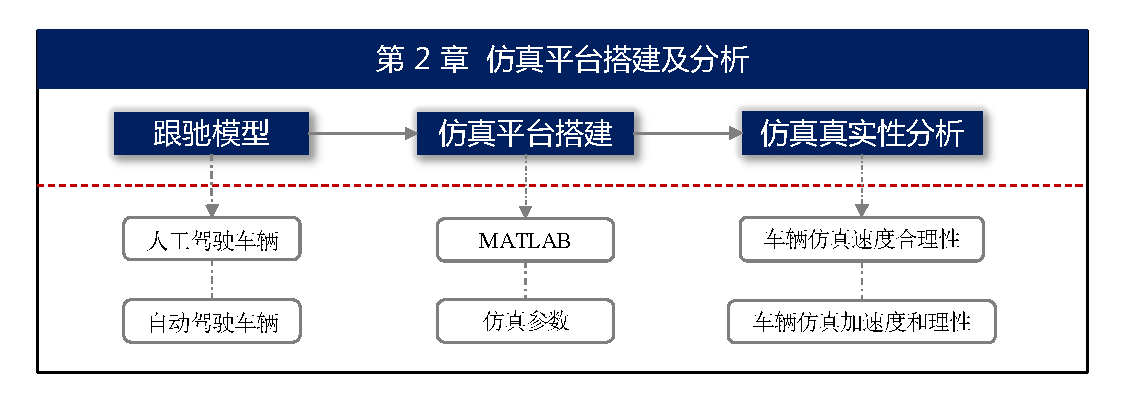
\includegraphics[width=1\linewidth]{chap02-1-structure.pdf}
  \caption{第2章结构}
  \label{fig:chap02-1-logic}
\end{figure}

\section{跟驰行为建模}

在本课题中,需要对人工驾驶和自动驾驶两种车辆的跟驰行为建模。

\subsection{人工驾驶车辆跟驰模型}

根据第一章中对跟驰行为建模研究现状的综述,对于人工驾驶车辆选择表达形式直观,参数量适中,对实际情况拟合情况较好的速度优化跟驰模型(OVM)。其具体表达式为

\begin{align}
  \dot{v}_n(t) &= \kappa \left\{ V \left[ h_n(t) \right] - v_n(t) \right\} \notag \\
  V \left[ h_n(t) \right] &= v_0 \left\{ 1 - \exp \left[ - \frac{\alpha}{v_0}\left(h_n(t)-s_0\right) \right] \right\}
  \label{eq:chap02-1}
\end{align}
其中,各符号含义在表\ref{tab:chap01-5}中给出,其相关参数取值如表\ref{tab:chap01-2}所示。

\begin{table}
  \centering
  \caption{速度优化跟驰模型参数取值}
  \begin{tabular}{cc}
    \toprule
    参数          &  取值                         \\
    \midrule
    敏感系数$\alpha$        & $0.999s^{-1}$         \\
    敏感系数$\kappa$       & $0.700s^{-1}$             \\
    自由流速度$v_0$             & $33.0 m/s$          \\
    最小安全距离$s_0$             & $1.62m$        \\
    \bottomrule
  \end{tabular}
  \label{tab:chap02-1}
\end{table}

下面对该跟驰模型进行简要分析。

速度优化函数描述了在当前车与前车的车头间距给定后,当前车驾驶员存在一个希望保持的理想的速度。图\ref{fig:chap02-2-OVM1}描述了这个理想速度的大小与两车车头距离的关系。
可以观察到速度优化函数在其定义域内是单调递增的,即前车距离越远,驾驶员希望保持的理想速度越大,以尽快缩小与前车的距离;当前车距离越近,驾驶员希望保持的理想速度越小,以减小
追尾的风险,这与真实情况是一致的。

\begin{figure}
  \centering
  \subcaptionbox{OVM速度优化函数图像\label{fig:chap02-2-OVM1}}
    {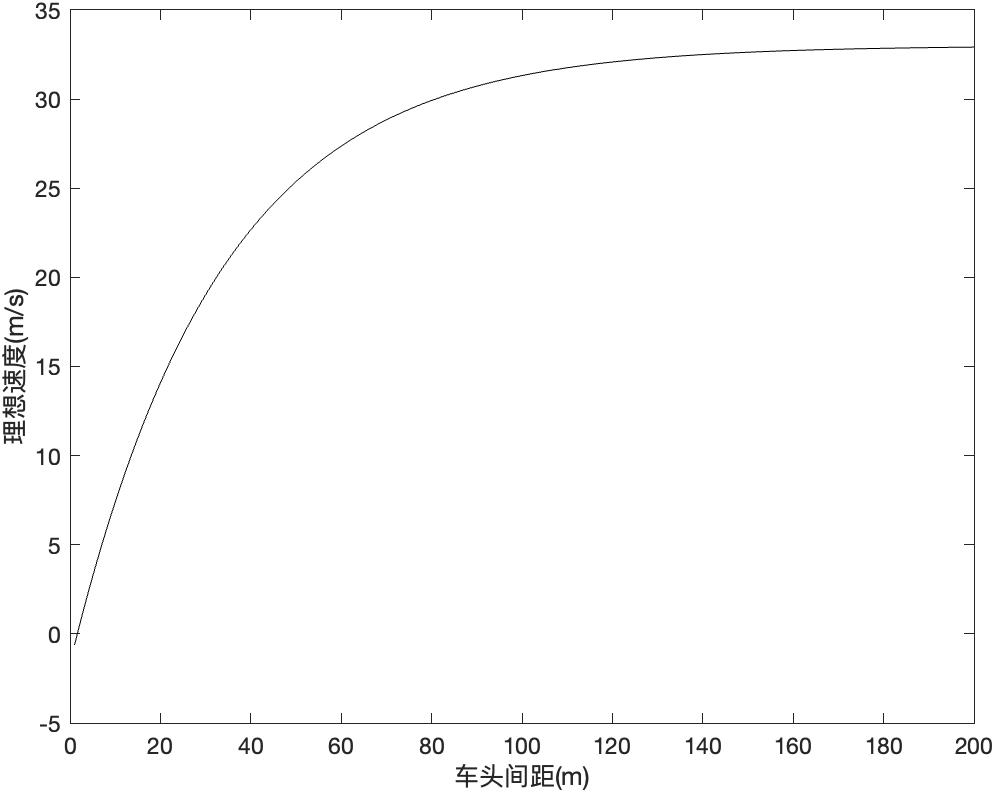
\includegraphics[width=0.45\linewidth]{chap02-2-OVM1.jpg}}
  \subcaptionbox{加速度与当前速度、车头间距的关系\label{fig:chap02-2-OVM2}}
    {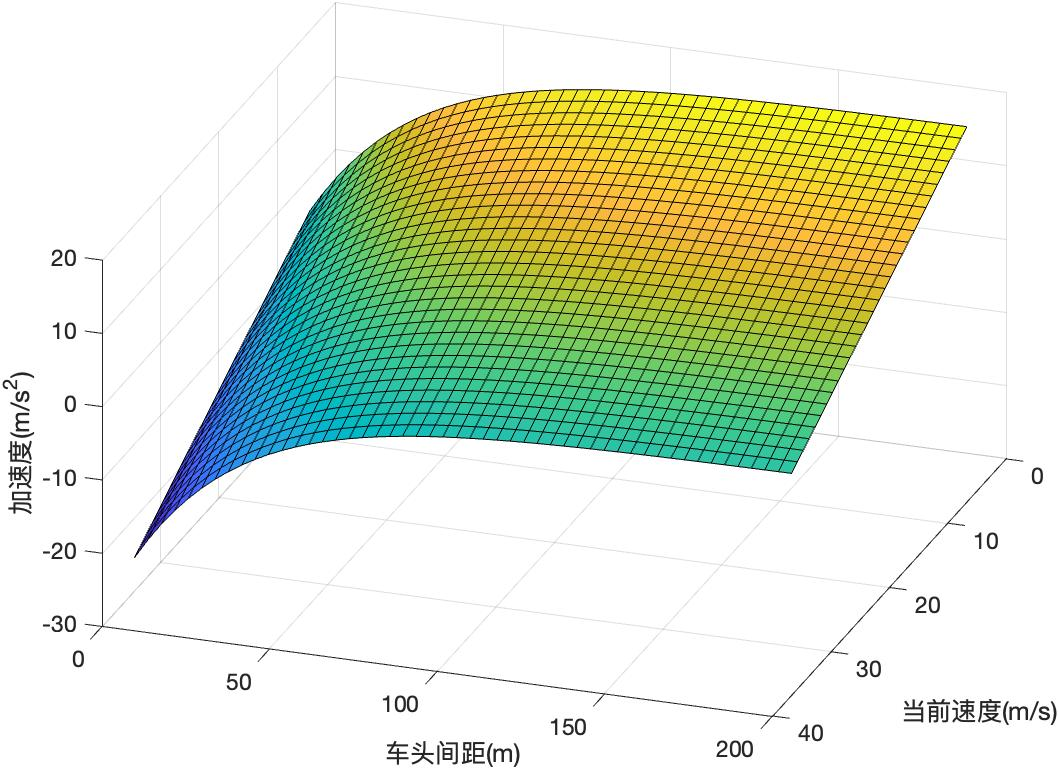
\includegraphics[width=0.5\linewidth]{chap02-2-OVM2.jpg}}
  \caption{OVM函数关系图像}
  \label{fig:chap02-2-OVM}
\end{figure}

图\ref{fig:chap02-2-OVM2}描述了车头时距、当前速度、加速度三者的关系。可以观察到当当前速度固定时,车头时距越大,加速度也越大,且呈现出与速度优化函数一样的增长规律,这与
式\ref{eq:chap02-1}是相符合的;当车头间距固定时,理想速度也就确定了,所以随着当前速度的增大,加速度线性减小。

\subsection{自动驾驶车辆跟驰模型}

自动驾驶车辆选择基于PID控制的车头时距控制算法来控制跟驰行为,该算法的表达式见式(\ref{eq:chap02-2})。
\begin{equation}
  \dot{v}_n(t) = k_1 \left[ h_n(t) - l - t_hv_n(t) \right] + k_2 \left[ v_{n-1}(t) - v_n(t) \right]
  \label{eq:chap02-2}
\end{equation}
其中,各符号含义在表\ref{tab:chap02-2}中给出

\begin{table}
  \centering
  \caption{基于PID控制的车头时距控制算法符号说明}
  \begin{tabular}{cc}
    \toprule
    符号          &  含义                         \\
    \midrule
    $k_1, k_2$            & 控制步长         \\
    $t_h$                 & 理想车头时距             \\
    $l$                   & 车身长度          \\
    $h_n(t)$              & 第$n$辆车在$t$时刻与前车的车头间距        \\
    $v_n(t)$              & 第$n$辆车在$t$时刻的速度 \\
    \bottomrule
  \end{tabular}
  \label{tab:chap02-2}
\end{table}

可以发现在该算法控制下,车辆的加减速由两部分控制。一是当前的两车车头距离与理想的车头距离的大小关系,如果当前两车车头距离小于理想的车头距离,那么参数$k_1$控制的部分倾向于减速;
二是当前车与前车的速度大小关系,如果当前车速度大于前车速度,$k_2$控制的部分倾向于减速。通过改变$k_1$和$k_2$的值,可以调节这两个部分的权重,二者综合即可决定当前车应当加速还是
减速,以及加速度的大小。


\section{仿真平台的搭建}

仿真基于MATLAB软件,模拟了一个由11辆车组成的车队,如图\ref{fig:chap02-3-simu1}所示。车队中的第一辆车是头车,其既不是人工驾驶车辆也不是自动驾驶车辆,而是按照实现规定好的策略行驶,即在0时刻以$-2m/s^2$的
加速度减速到原速度的$90\%$,紧接着以$2m/s^2$的加速度恢复元素,其速度变化情况如图\ref{fig:chap02-3-simu2}所示。如此设置头车是为了加入扰动,虽扰在真实场景下扰动可能发生在车队中的任何一辆车上,由于受到
该扰动影响的车辆是此车之后的车辆,只要将此车看作头车,就与仿真实验场景一致了,所以这样的仿真情景具有一定的一般性。

\begin{figure}
  \centering
  \subcaptionbox{车队示意图\label{fig:chap02-3-simu1}}
    {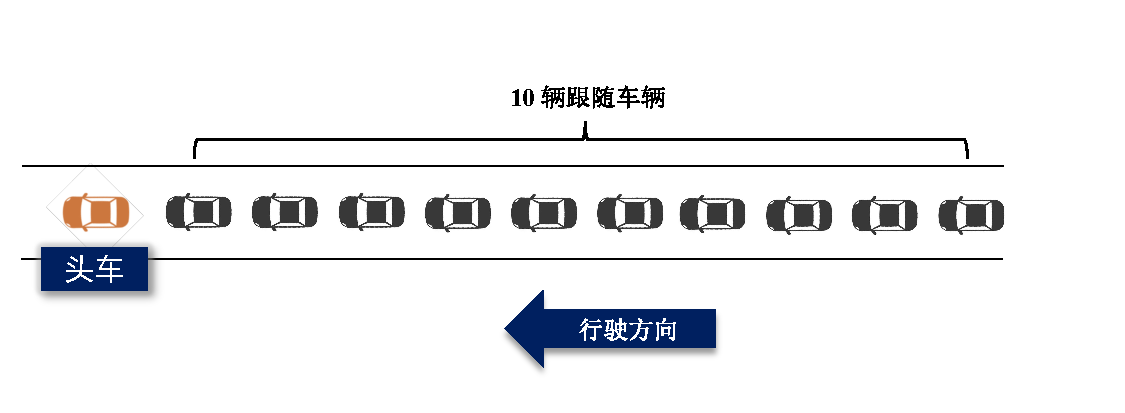
\includegraphics[width=1\linewidth]{chap02-3-simu1.pdf}}
  \subcaptionbox{头车速度变化曲线(初速度$20m/s$,截取前$10s$)\label{fig:chap02-3-simu2}}
    {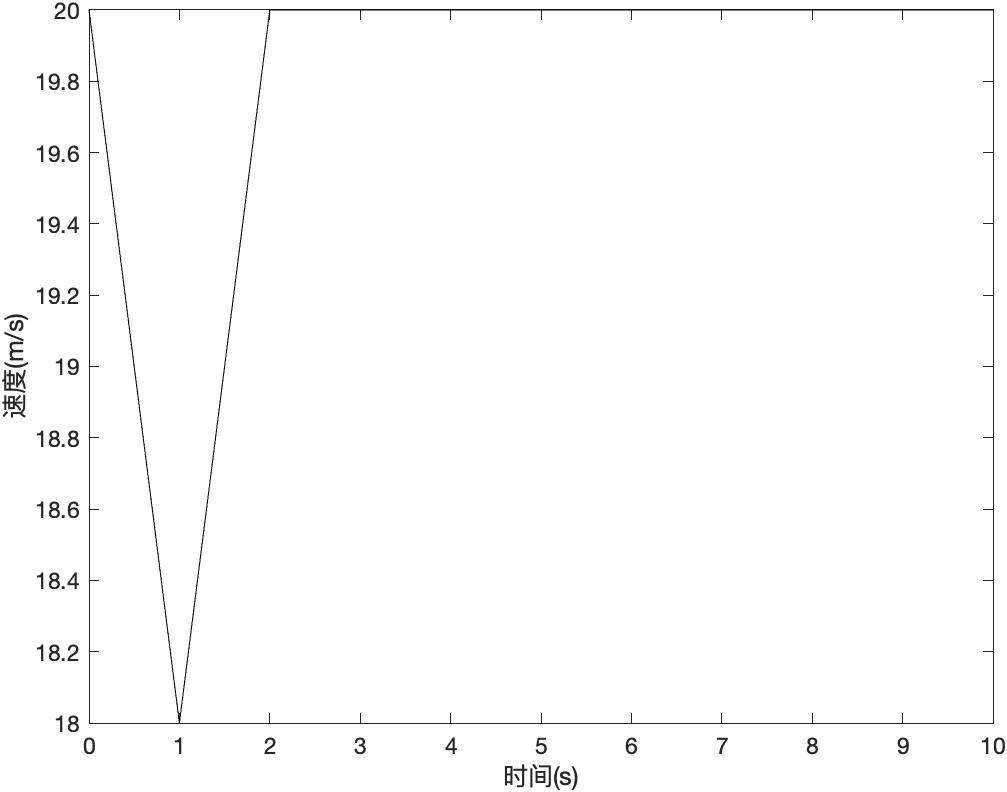
\includegraphics[width=0.6\linewidth]{chap02-3-simu2.jpg}}
  \caption{仿真场景设置}
  \label{fig:chap02-2-simu}
\end{figure}

为了数值仿真只能模拟,首先将连续场景离散化。为了尽量减小误差,仿真步长取$0.01s$,总仿真时长为$500s$,这意味着有50000个采样点。

为了使仿真尽可能的接近真实情况,也应考虑实际情况中的物理限制,如真实场景下车辆的加速度大小是限制在一定范围内的,这由轮胎与道路摩擦因数等原因决定。


\section{仿真平台真实性分析}


% !TeX root = ../thuthesis-example.tex

\chapter{混合车队队列稳定性分析}
\label{sec:3}

\section{人工驾驶车辆扰动传递函数推导}

人工驾驶车辆的跟驰行为由速度优化模型(OVM)描述,其具体表达式为

\begin{align}
  \dot{v}_n(t) &= \kappa \left\{ \mathrm{V} \left[ h_n(t) \right] - v_n(t) \right\} \notag \\
  \mathrm{V} \left[ h_n(t) \right] &= v_0 \left\{ 1 - \exp \left[ - \frac{\alpha}{v_0}\left(h_n(t)-s_0\right) \right] \right\}
  \label{eq:chap03-1}
\end{align}
其中,各符号含义在表\ref{tab:chap01-5}中给出,其相关参数取值如表\ref{tab:chap02-1}所示。

当车队整体处于均衡状态时,车队中所有车辆加速度都保持为0,所有车辆都保持均衡速度$v_e$行驶。对于人工驾驶车辆,说明速度优化函数与车队均衡速度相同,即
\begin{equation}
  \mathrm{V}[h_e] = v_e
  \label{eq:chap03-2}
\end{equation}
其中$h_e$为均衡状态下自动驾驶车辆与前车的距离,称作均衡速度。将速度优化函数带入式(\ref{eq:chap03-2}),得到式(\ref{eq:chap03-3})。
\begin{equation}
  v_0 \left\{ 1 - \exp \left[ -\frac{\alpha}{v_0} (h_e - s_0) \right] \right\} = v_e
  \label{eq:chap03-3}
\end{equation}
整理得到均衡距离与均衡速度之间的关系,如式(\ref{eq:chap03-4})所示。
\begin{equation}
  h_e = s_0 - \frac{v_0}{\alpha}\ln\left( 1 - \frac{v_e}{v_0} \right)
  \label{eq:chap03-4}
\end{equation}

图\ref{fig:chap03-1}描述了均衡距离与均衡速度的关系,从中可以看出OVM的均衡距离与均衡速度呈正相关,均衡速度越大,两车之间的均衡距离也越大,这说明当速度较大时,驾驶员倾向于
增大与前车的距离以减小追尾的风险。同时也可以看出随着均衡速度的增加,均衡距离的增长速度也越来越快。

\begin{figure}
  \centering
  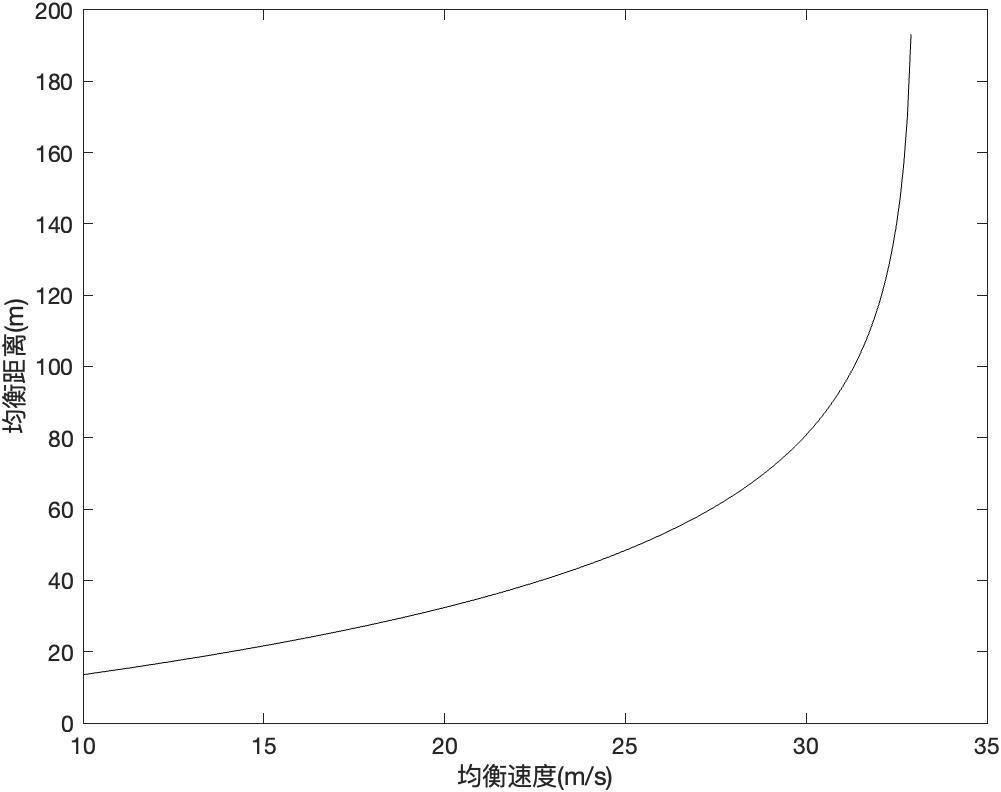
\includegraphics[width=0.5\linewidth]{chap03-1.jpg}
  \caption{OVM均衡距离与均衡速度关系曲线}
  \label{fig:chap03-1}
\end{figure}

下面对OVM的人工驾驶车辆对扰动的传递情况进行分析。假设车队受到扰动,第$n-1$辆车和第$n$辆车的扰动为
\begin{equation}
  \begin{cases}
    \increment{v_{n-1}(t)} = v_{n-1}(t) - v_e \\
    \increment{v_n(t)} = v_n(t) - v_e
  \end{cases}
  \label{eq:chap03-5}
\end{equation}
对等式两边同时求导,可以发现扰动函数的导函数与速度函数的导函数是相同的,即
\begin{equation}
  \begin{cases}
    \increment{\dot{v}_{n-1}(t)} = \dot{v}_{n-1}(t) \\
    \increment{\dot{v}_n(t)} = \dot{v}_n(t)
  \end{cases}
  \label{eq:chap03-6}
\end{equation}
将式(\ref{eq:chap03-1})中加速度函数中的速度优化函数在$h_n(t)=h_e$处一阶泰勒展开,得到式(\ref{eq:chap03-7})
\begin{equation}
  \increment{\dot{v}}_n(t) = \dot{v}_n(t) = \kappa \left\{ \mathrm{V'}(h_e)[h_n(t)-h_e] - v_n(t) \right\}
  \label{eq:chap03-7}
\end{equation}
等式两边同时求导,得到
\begin{equation}
  \begin{aligned}
    \increment{\ddot{v}}_n(t) &= \kappa \left[ \mathrm{V'}(h_e)\dot{h}_n(t) - \dot{v}_n(t) \right] \\
                              &= \kappa \left\{ \mathrm{V'}(h_e)\left[v_{n-1}(t) - v_n(t)\right] - \dot{v}_n(t) \right\} \\
                              &= \kappa \left\{ \mathrm{V'}(h_e)\left[\increment{v_{n-1}(t)} - \increment{v_n(t)} \right] - \increment{\dot{v}_n(t)} \right\}
  \end{aligned}       
  \label{eq:chap03-8}
\end{equation}
等式两边同时做拉普拉斯变换(因为是在均衡状态下添加的扰动,所以满足零初始条件),得到
\begin{equation}
  s^2\increment{V}_n(s) = \kappa \left\{ \mathrm{V'}(h_e)\left[\increment{V_{n-1}(s)} - \increment{V_n(s)} \right] - s\increment{V_n(s)} \right\}
  \label{eq:chap03-9}
\end{equation}
整理得到速度扰动在OVM下的传递函数$G_{H}(s)$如式(\ref{eq:chap03-10})所示。
\begin{equation}
  G_{H}(s) = \frac{\increment{V_{n}(s)}}{\increment{V_{n-1}(s)}} = \frac{\kappa V'(h_e)}{s^2 + \kappa s + \kappa V'(h_e)}
  \label{eq:chap03-10}
\end{equation}

\section{自动驾驶车辆扰动传递函数推导}

自动驾驶车辆的跟驰行为由基于PID控制的车头时距控制算法控制,该算法的表达式为
\begin{equation}
  \dot{v}_n(t) = k_1 \left[ h_n(t) - l - t_hv_n(t) \right] + k_2 \left[ v_{n-1}(t) - v_n(t) \right]
  \label{eq:chap03-11}
\end{equation}
其中,各符号含义在表\ref{tab:chap02-2}中给出

下面对自动驾驶车辆对扰动的传递情况进行分析。与人工驾驶车辆分析过程相同,假设车队受到扰动,第$n-1$辆车和第$n$辆车的扰动为
\begin{equation}
  \begin{cases}
    \increment{v_{n-1}(t)} = v_{n-1}(t) - v_e \\
    \increment{v_n(t)} = v_n(t) - v_e
  \end{cases}
  \label{eq:chap03-12}
\end{equation}
扰动函数的导函数与速度函数的导函数是相同的,即
\begin{equation}
  \begin{cases}
    \increment{\dot{v}_{n-1}(t)} = \dot{v}_{n-1}(t) \\
    \increment{\dot{v}_n(t)} = \dot{v}_n(t)
  \end{cases}
  \label{eq:chap03-13}
\end{equation}
对式(\ref{eq:chap03-11})两边同时求导,得到
\begin{equation}
  \begin{aligned}
    \increment{\ddot{v}}_n(t) &= \ddot{v}_n(t) = k_1 [\dot{h}_n(t) - t_h\dot{v}_n(t)]
                              + k_2 [\dot{v}_{n-1}(t) - \dot{v}_n(t)] \\
    &= k_1 [\dot{h}_n(t) - t_h \increment{\dot{v}_n(t)}]
       + k_2 [\increment{\dot{v}_{n-1}(t)} - \increment{\dot{v}_n(t)}] \\
    &= k_1 [\increment{v}_{n-1}(t) - \increment{v}_n(t) - t_h \increment{\dot{v}_n(t)}]
       + k_2 [\increment{\dot{v}_{n-1}(t)} - \increment{\dot{v}_n(t)}] \\
  \end{aligned}
  \label{eq:chap03-14}
\end{equation}
等式两边同时做拉普拉斯变换,得到
\begin{equation}
  \begin{aligned}
    s^2\increment{V}_n(s) = &k_1[ \increment{V_{n-1}(s)} - \increment{V_{n}(s)} - t_hs\increment{V_{n}(s)}] \\
                            &+ k_2 [ s\increment{V_{n-1}(s)} - s\increment{V_n(s)} ]
  \end{aligned}
  \label{eq:chap03-15}
\end{equation}
整理得到速度扰动在自动驾驶车辆的传递函数$G_{A}(s)$如式(\ref{eq:chap03-16})所示。
\begin{equation}
  G_{H}(s) = \frac{\increment{V_{n}(s)}}{\increment{V_{n-1}(s)}} = 
  \frac{k_2s + k_1}{s^2 + (k_1t_h + k_2) s + k_1}
  \label{eq:chap03-16}
\end{equation}

\section{混合车队跟驰行为稳定性分析}
\label{sec:3.3}

首先给出队列稳定性的定义。 \\

\begin{definition}[队列稳定(String Stable)]
  对于一个跟驰车队,如果头车受到扰动后,扰动沿着车队逐渐衰减,认为该车队是队列稳定的。
  \label{def:chap03-def1}
\end{definition}

根据\ref{sec:1.2.2}中对车队稳定性分析研究现状的调研,得到只包含一种传递函数的车队的队列稳定性充分条件为
\begin{equation}
  | G(j\omega) | < 1
  \label{eq:chap03-17}
\end{equation}
其中$G(j\omega)$是该车队含有的唯一一种传递函数。这个充分条件其实是由式(\ref{eq:chap03-18})简化而来的。
\begin{equation}
  | G(j\omega) |^n < 1
  \label{eq:chap03-18}
\end{equation}
其中$n$是车队中跟驰车辆的数量。

对于含有两种及两种以上传递函数的车队,比如本工作中人工驾驶车辆和自动驾驶车辆有不同的传递函数,车队队列稳定的充分条件是
\begin{equation}
  \left\Vert \prod_{i=1}^{m}{G_i(j\omega)^{p_i}} \right\Vert_{\infty} < 1
  \label{eq:chap03-19}
\end{equation}
其中,车队中传递函数共有$m$种,第$i$种传递函数对应的车辆在车队跟驰车辆中的比例为$p_i$。

对于本工作的情景,队列稳定的条件可以简化为
\begin{equation}
  \left\Vert G(j\omega) \right\Vert_{\infty} = \left\Vert G_H(j\omega)^{1-p} \cdot G_A(j\omega)^p \right\Vert_{\infty} < 1
  \label{eq:chap03-20}
\end{equation}

需要说明的是,只有在车队中每一辆跟驰车辆都严格按照其跟驰模型行驶的情况下,式(\ref{eq:chap03-20})才能保证车辆绝对队列稳定,该队列稳定性的判据的价值更多
体现在理论层面,因为在真实场景下,跟驰车辆并不会严格按照某一个跟驰模型行驶,即使是自动驾驶车辆,也会因为计算误差、传感器精确度、计算延迟等众多实际因素产生
与其控制算法的误差,更何况真实场景下,交通环境中存在大量的随机性。

对于本工作,如\ref{sec:simulation-platform}中提到的,在搭建仿真平台时,为了追求更加接近真实场景的仿真,加入了加速度限制、人类驾驶员反应延迟、一阶惯性环节等
使仿真跟驰行为不同于其跟驰模型的因素,使得仿真环境也是不同于每一辆跟驰车辆都严格按照其跟驰模型行驶的理想情况的。

但这并不意味着以上的推导是没有意义的,一方面,混合车队的队列稳定性充分条件的推导具有理论价值;另一方面,对于仿真场景或真实场景,式(\ref{eq:chap03-20})中
$\left\Vert G(j\omega) \right\Vert_{\infty}$的值仍能反应车队的队列稳定情况,即在真实场景中,满足式(\ref{eq:chap03-20})可以说明该车队在理论上队列稳定,
但真实场景下仍然有出现扰动被不断放大的可能,即便如此,我们仍可以用$\left\Vert G(j\omega) \right\Vert_{\infty}$的值作为一个指标对车队的队列稳定性进行评估。


\section{混合车队跟驰行为稳定性仿真验证}
\label{sec:3.3}

在本小节中,将通过仿真的方式对\ref{sec:3.3}中理论推导的结果进行验证。需要说明的是,本小节的仿真分为两部分,一部分是理想情况仿真,是对理论推导结果的验证,在仿真过程中没有加入\ref{sec:simulation-platform}
中提到的加速度限制、人类驾驶员反应延迟、一阶惯性环节等使仿真跟驰行为不同于其跟驰模型的因素;另一部分是模拟真实场景仿真,在仿真过程中加入了使仿真跟驰行为不同于其跟驰模型的因素,是为了说明式(\ref{eq:chap03-20})
得到的指标确实可以反应模拟真实场景下车队的稳定性。

\subsection{车队稳定情况仿真}

理论上,队列稳定的车队在受到扰动后,扰动会逐渐减小,最终趋于0。下面选取一个场景对车队稳定的情况进行仿真。\\

经验证,在自动驾驶车辆占比为0.5,初始均衡速度为$25m/s$的条件下,$\left\Vert G(j\omega) \right\Vert_{\infty} = \left\Vert G_H(j\omega)^{0.5} \cdot G_A(j\omega)^{0.5} \right\Vert_{\infty} < 1$,
即理论上车队是稳定的。

\begin{figure}
  \centering
  \subcaptionbox{理想情况仿真 \label{fig:chap03-2-stable-ideal}}
    {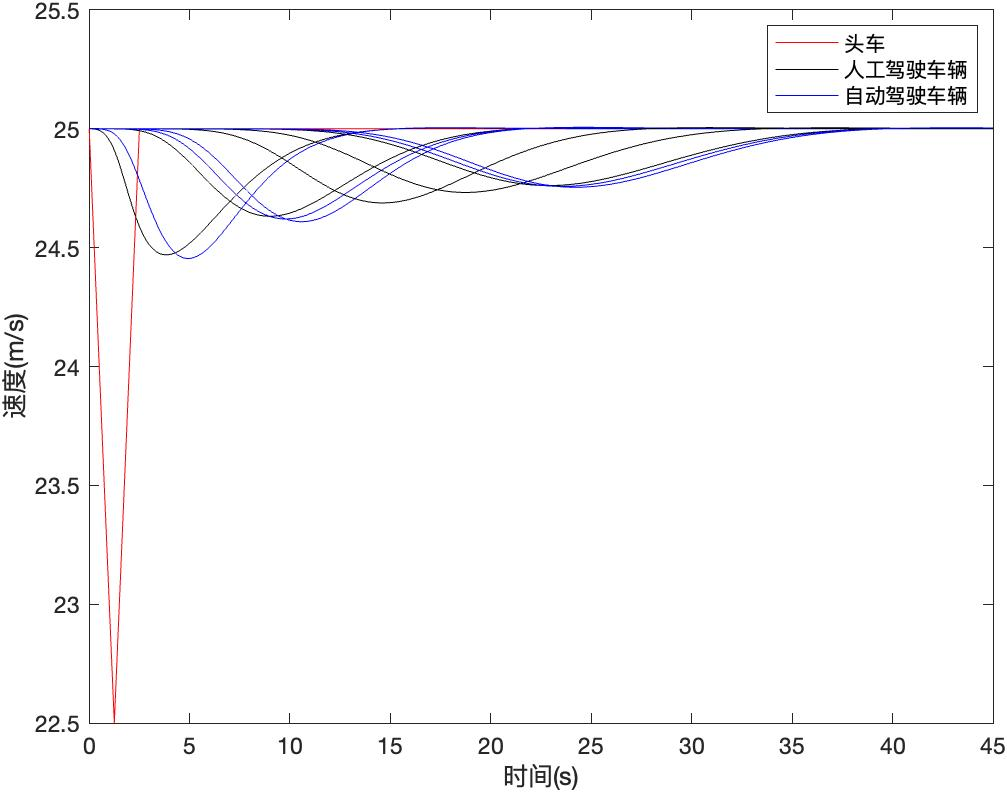
\includegraphics[width=0.47\linewidth]{chap03-2-ideal-0.5-25.jpg}}
  \subcaptionbox{模拟真实场景仿真 \label{fig:chap03-2-stable-real}}
    {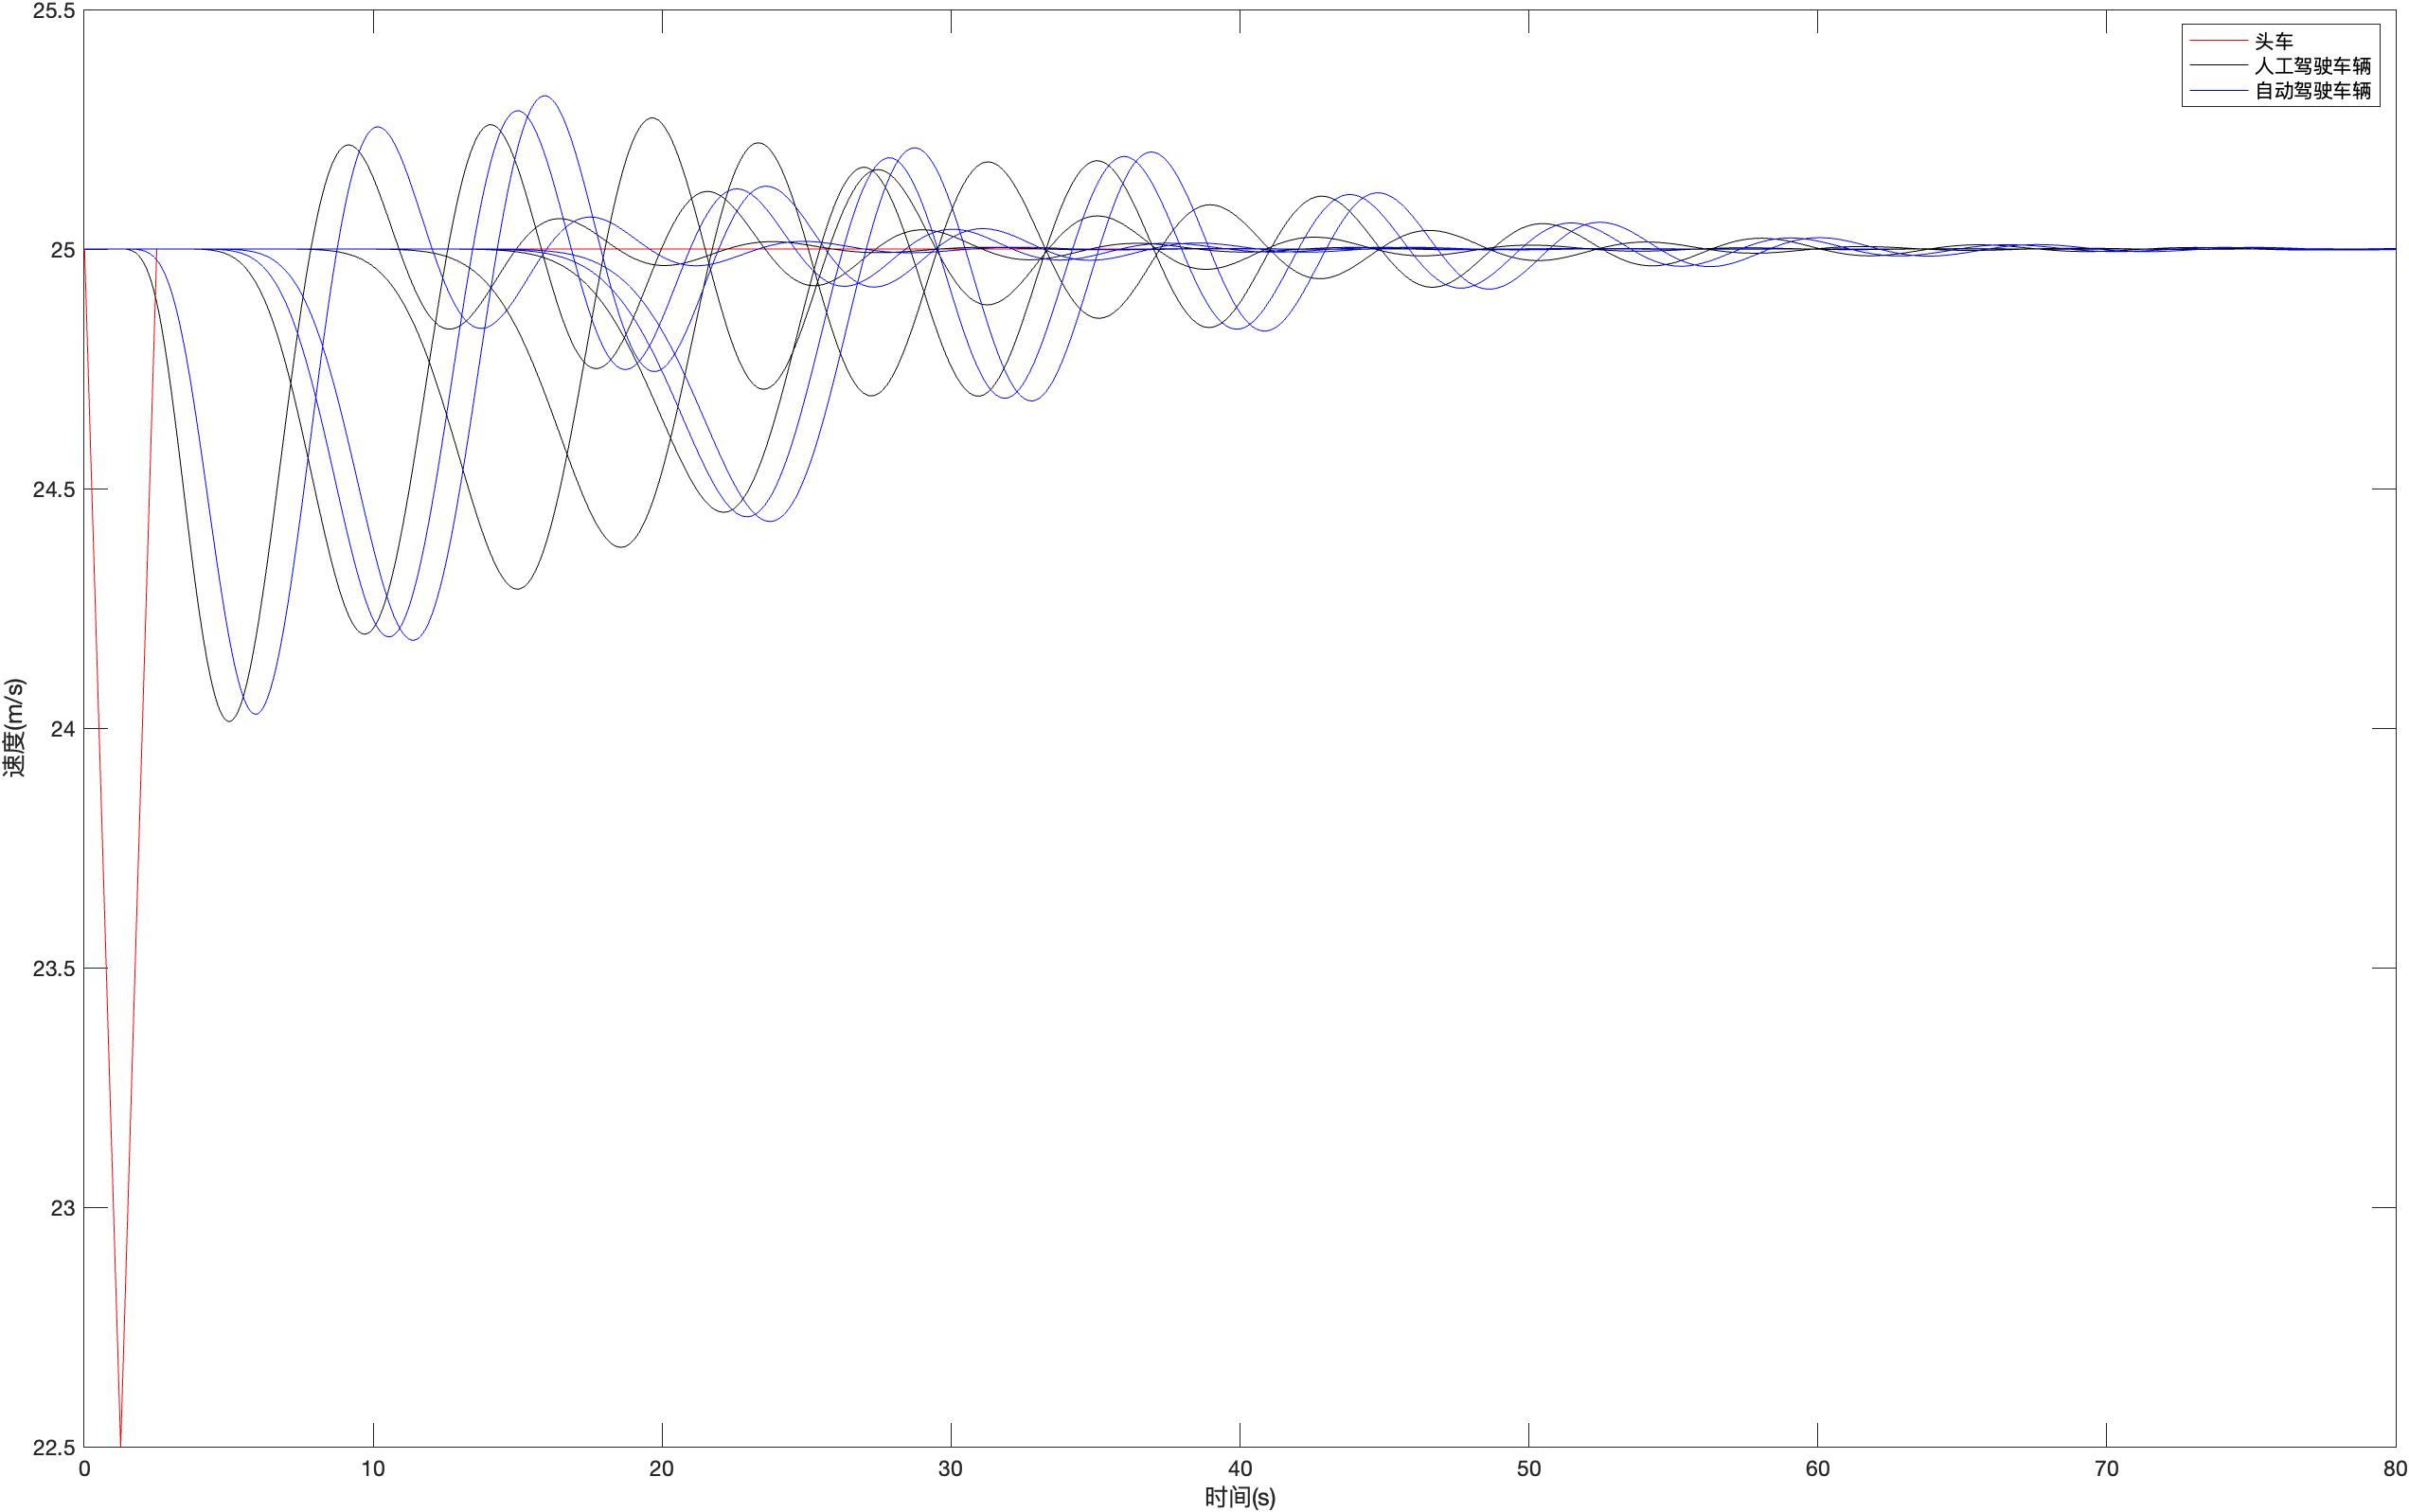
\includegraphics[width=0.52\linewidth]{chap03-2-real-0.5-25.jpg}}
    \caption*{在理想情况仿真中,车队中每辆跟驰车辆严格按照跟驰模型行驶;在模拟真实场景仿真中,加入了加速度限制、人类驾驶员反应延迟、一阶惯性环节等因素}
    \caption{车队稳定情况仿真}
  \label{fig:chap03-2}
\end{figure}

可以观察到无论是在理想情况仿真中还是在模拟真实场景仿真中,衰减都沿着车队逐渐衰减,这说明二者对应的车队都是稳定的。

\subsection{车队不稳定情况仿真}
\label{sec:3.4.2}

经验证,在自动驾驶车辆占比为0.3,初始均衡速度为$10m/s$的条件下,$\left\Vert G(j\omega) \right\Vert_{\infty} = \left\Vert G_H(j\omega)^{0.7} \cdot G_A(j\omega)^{0.3} \right\Vert_{\infty} > 1$,
即理论上车队是不稳定的。

\begin{figure}
  \centering
  \subcaptionbox{理想情况仿真 \label{fig:chap03-3-unstable-ideal}}
    {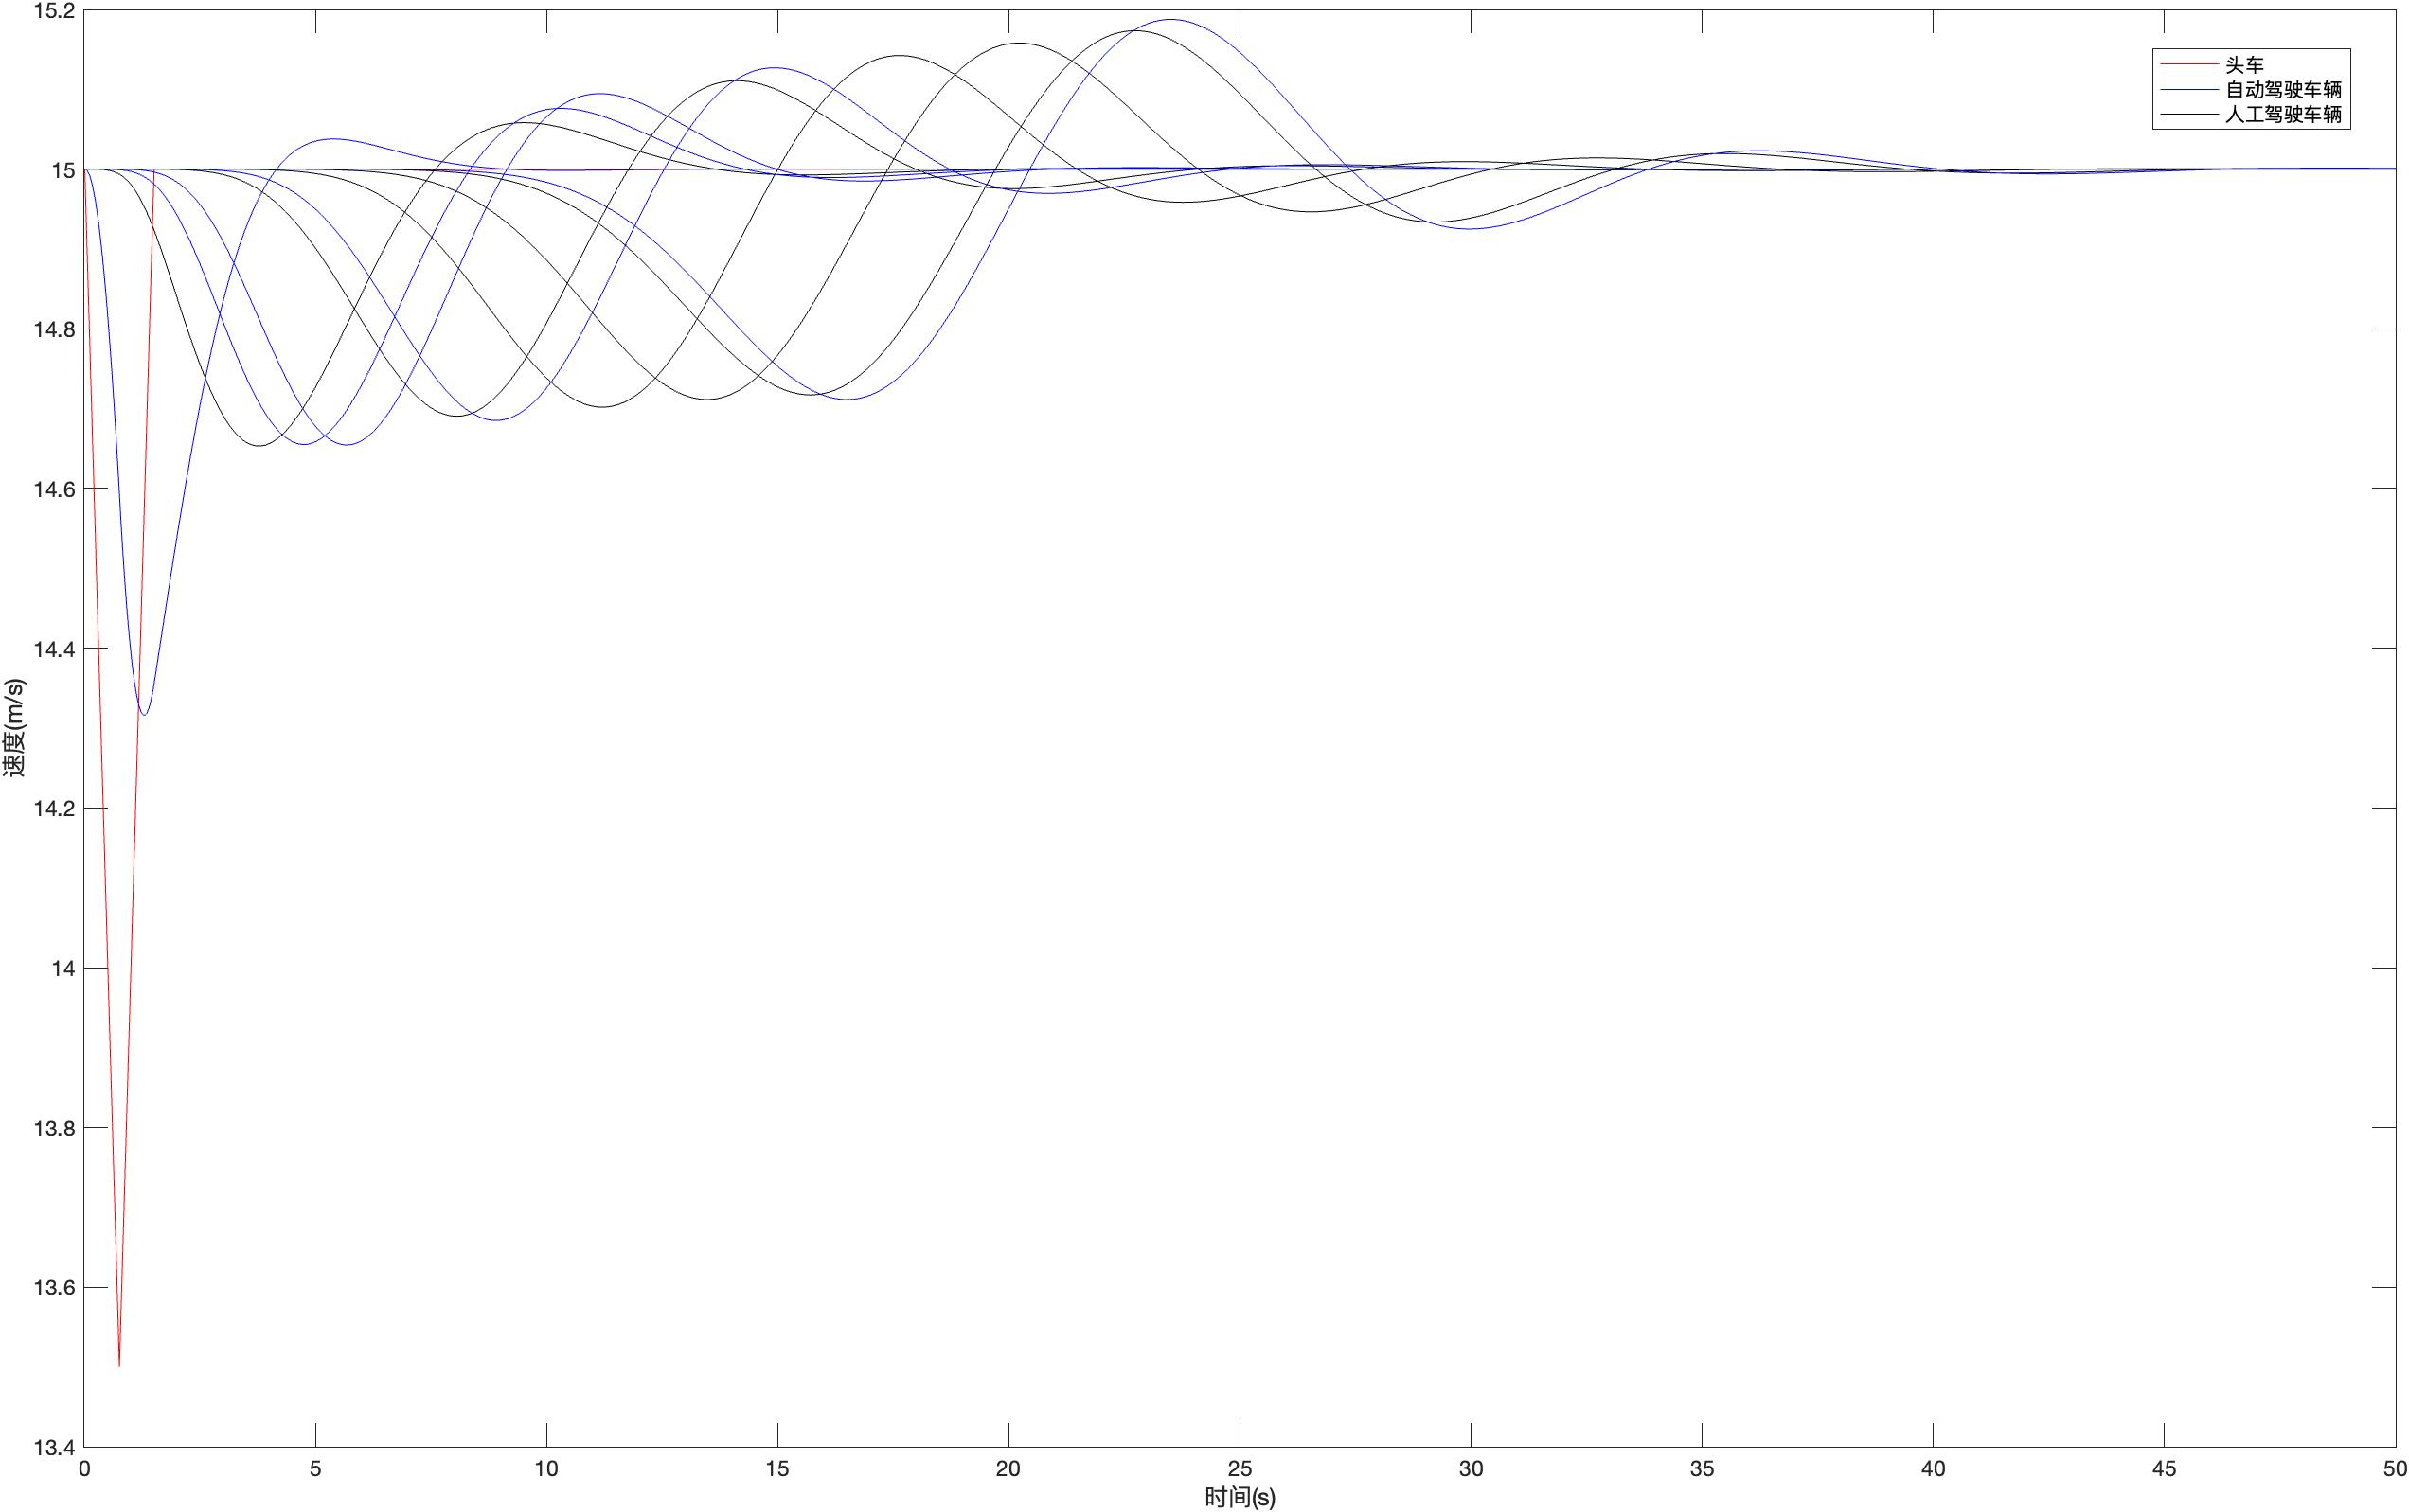
\includegraphics[width=0.5\linewidth]{chap03-2-ideal-0.5-15.jpg}}
  \subcaptionbox{模拟真实场景仿真 \label{fig:chap03-3-unstable-real}}
    {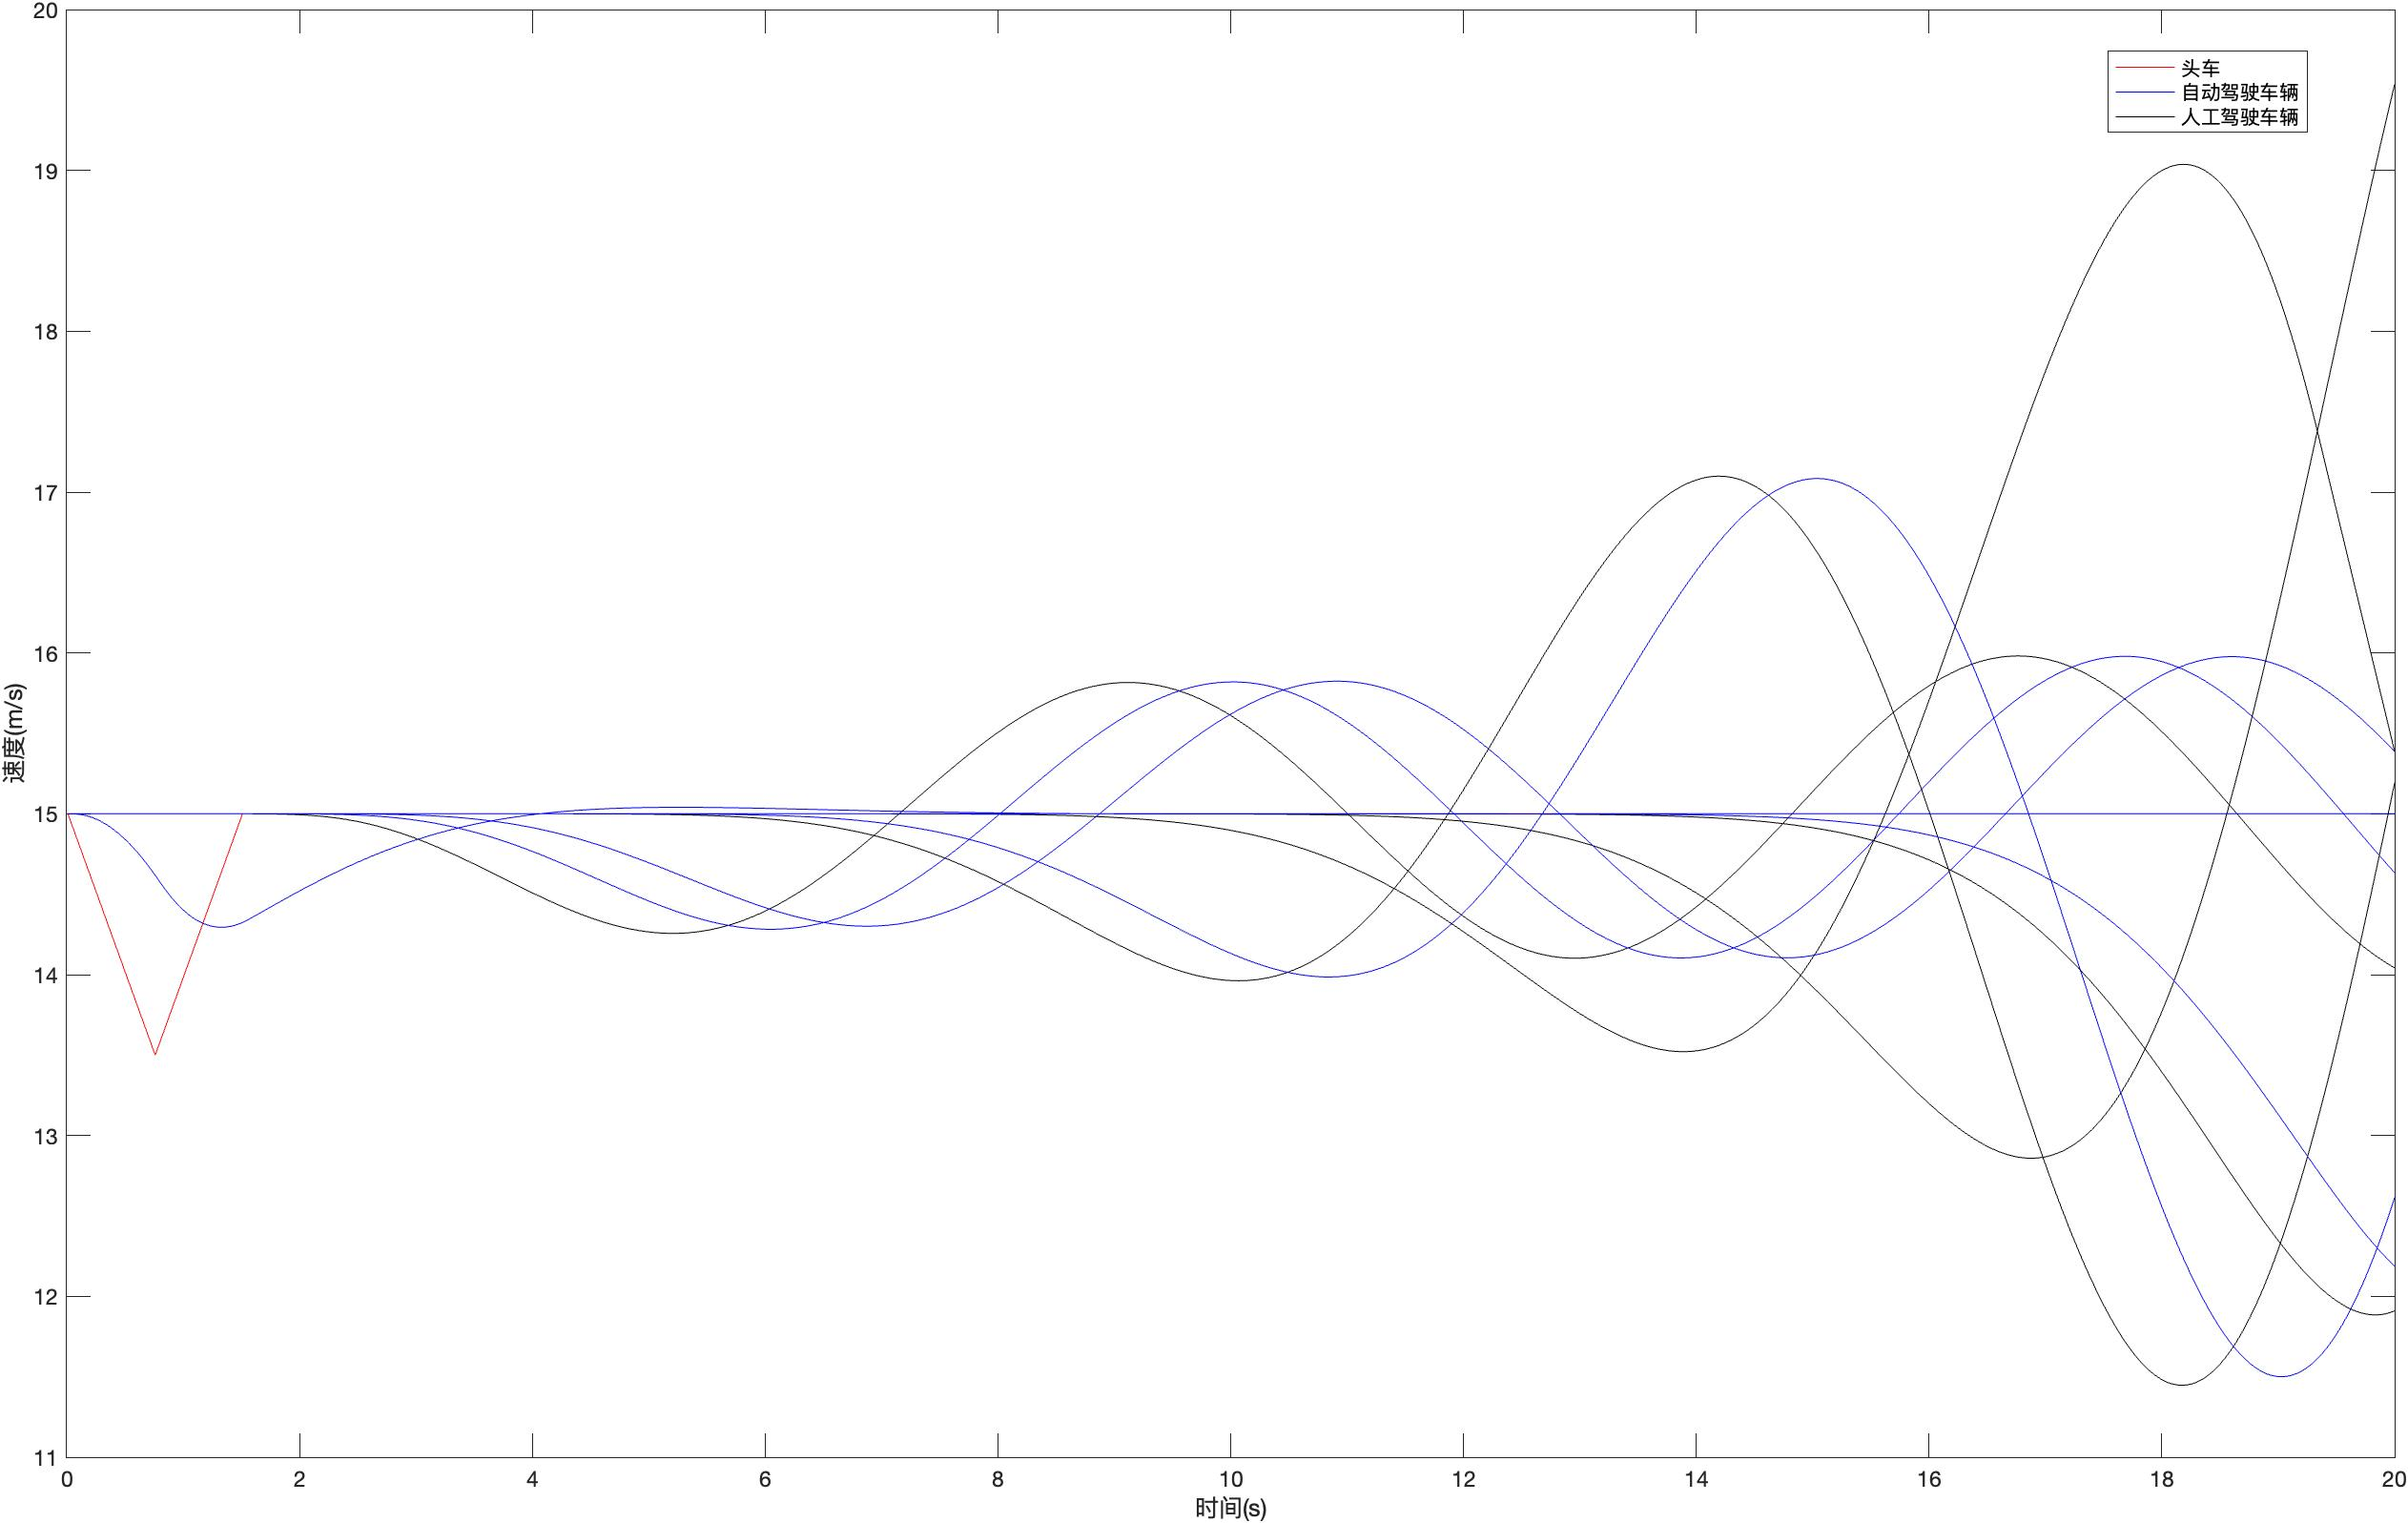
\includegraphics[width=0.5\linewidth]{chap03-3-real-0.5-15.jpg}}
    \caption*{在理想情况仿真中,车队中每辆跟驰车辆严格按照跟驰模型行驶;在模拟真实场景仿真中,加入了加速度限制、人类驾驶员反应延迟、一阶惯性环节等因素}
    \caption{车队不稳定情况仿真}
  \label{fig:chap03-3}
\end{figure}

可以观察到在理想情况仿真中,虽然随着时间的推移,车队中每辆车的扰动都趋于0,但从空间角度来看,衰减沿着车队被放大,通过队列稳定性的定义,可以确定这个车队是队列不稳定的。而
对于模拟真实场景仿真中,衰车队呈现出更不稳定的状态,扰动最终发散,在这样的车队中极容易发生事故。

但在图\ref{fig:chap03-2}和图\ref{fig:chap03-3}所示的场景中,理想情况仿真和模拟真实场景仿真都具有一致的稳定性,虽然这并不意味着理想情况和模拟真实场景情况有相同的稳定性,但可以说明
式(\ref{eq:chap03-20})得到的车队传递函数无穷范数即使在考虑了真实场景因素的情况下,也能反应车队整体的队列稳定性。

\section{本章小结}
在本章中,首先对人工驾驶车辆和自动驾驶车辆对扰动对传递情况进行了分析,得到了二者关于扰动大小的传递函数,进而利用队列稳定性这一概念推导得到了理论上车队达到队列稳定的充分条件。但这一条件也存在一定的局限性,
即只有当车队中所有车辆都严格按照其跟驰模型行驶时,才能使用这个判据,而本工作的核心是建立车队稳定性与碰撞风险之间的联系,碰撞风险是基于仿真得到的,如果仿真场景不够真实,则建立的联系就不具备实际价值。所以
在本章的最后对理想情况和模拟真实场景都进行了仿真分析,发现$\left\Vert G(j\omega) \right\Vert_{\infty}$的值能够反应真实场景下车队的稳定程度,也说明了本章进行的稳定性分析工作是有意义的。

图\ref{fig:chap03-4}描述了本章的结构。

\begin{figure}
  \centering
  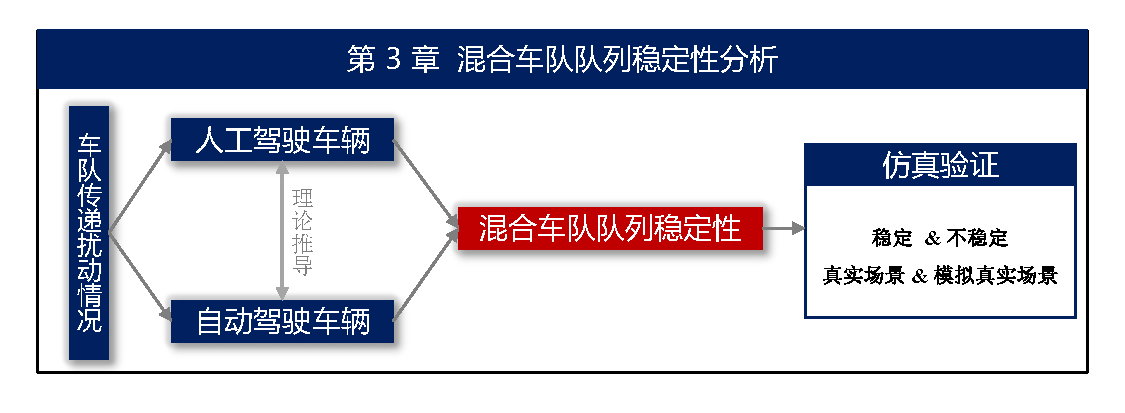
\includegraphics[width=1\linewidth]{chap03-structure.pdf}
  \caption{第3章结构}
  \label{fig:chap03-4}
\end{figure}
% !TeX root = ../thuthesis-example.tex

\chapter{混合车队稳定性与碰撞风险关系探究}

\section{仿真中碰撞发生情况分析}
\label{sec:4.1}

在仿真中,会改变自动驾驶车辆的比例$p$和初始均衡速度$v_e$,进行若干次实验, 虽然仿真实验的时长设置为$500s$,但不是每次实验都能够进行$500s$,这是因为在实验过程中会出现碰撞的情况,在所有仿真实验中,一旦发生了碰撞,该实验将终止。

之所以首先要对碰撞的情况进行分析是因为对于碰撞和非碰撞的样本,衡量其碰撞风险的方式也完全不同。对于发生了碰撞的实验样本,会更加关注碰撞发生的时间以及追尾车辆的分布情况;而对于没有发生碰撞的实验样本,会更加关注整个实验过程车队中蕴含的潜在危险。其实对于碰撞样本与非碰撞样本,对于稳定性的描述指标也是不同的,这将在后面小节进行介绍。

通过仿真发现,发生碰撞并不是一个小概率事件。直观上,是否发生碰撞与车队的稳定性之间存在相关性。

正如在\ref{sec:3.4.2}中提到的,车队整体传递函数的无穷范数能够反应真实场景下车队的稳定程度,于是此处定义第一个车队队列稳定性指标$G_{max}$。
\begin{equation}
    G_{max}(p, v_e) = \left\Vert G_H(j\omega)^{1-p} \cdot G_A(j\omega)^p \right\Vert_{\infty}
    \label{eq:chap04-1}
\end{equation}
其中,各参数含义在表\ref{tab:chap04-1}中列出

\begin{table}
    \centering
    \caption{队列稳定性指标$G_{max}$符号含义说明}
    \begin{tabular}{cc}
      \toprule
      符号          &  含义                         \\
      \midrule
      $G_H(j\omega)$    & 人工驾驶车辆传递函数        \\
      $G_A(j\omega)$    & 自动驾驶车辆传递函数         \\
      $p$               & 车队中自动驾驶车辆比例       \\
      $v_e$             & 车队的初始均衡速度          \\
      \bottomrule
    \end{tabular}
    \label{tab:chap04-1}
  \end{table}

正如式(\ref{eq:chap04-1})所示,指标$G_{max}$在人工驾驶车辆和自动驾驶车辆传递函数参数均确定下来之后,是车队中自动驾驶车辆比例$p$和车队的初始均衡速度$v_e$的函数。图
\ref{fig:chap04-1}所示是该二元函数的函数图像。 \\\\

\begin{figure}
    \centering
    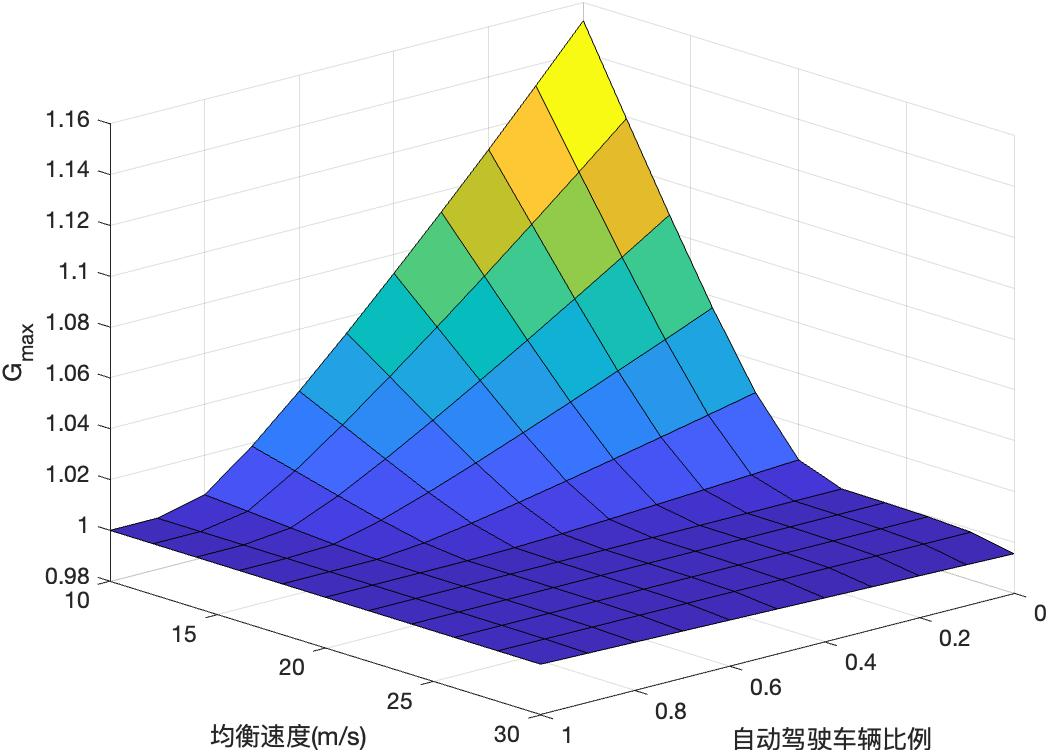
\includegraphics[width=0.9\linewidth]{chap04-Gmax.jpg}
    \caption{$G_{max}$函数图像}
    \label{fig:chap04-1}
\end{figure}

可以发现总体上,当固定自动驾驶车辆比例$p$,$G_{max}$随着初始均衡速度$v_e$的增大而减小;当固定初是均衡速度$v_e$,$G_{max}$随着自动驾驶车辆比例$p$的增大而减小。
因为$G_{max}$描述的是车队中车头受到的扰动到队尾的传递情况,所以可以认为$G_{max}$越大,车队的队列稳定性越差,反之,则相反。于是可以认为,对于一个混合车队,自动驾驶
车辆比例越大,初始的均衡速度越大,车队的队列稳定性越好。

另一方面,可以发现在选定的跟驰模型参数下,$G_{max}$的值多大于等于1,即对理论上不稳定的样本会有较好的描述,而由于稳定的样本的$G_{max}$取值集中在一个较小的区间,所以
在该指标下的区分度并不是很好。

下面通过仿真实验探究碰撞的发生与车队稳定性之间的关系。实验设计为:自动驾驶车辆比例$p$以0.1的步长遍历0到1,对于每一个$p$的取值,初始均衡速度以$2m/s$的步长遍历$10m/s$
到$30m/s$,对于每一组$(p, v_e)$取值,计算其$G_{max}$,并统计碰撞发生的频率。需要说明的是,即使确定了$p$和$v_e$的取值,车队仍有$\binom{10}{10\times p}$种排列,不同的排列
虽然$G_{max}$取值相同,但碰撞情况可能不同,这里的碰撞发生的频率就是指发生了碰撞的排列占所有排列的比例。 \\\\

\begin{figure}
    \centering
    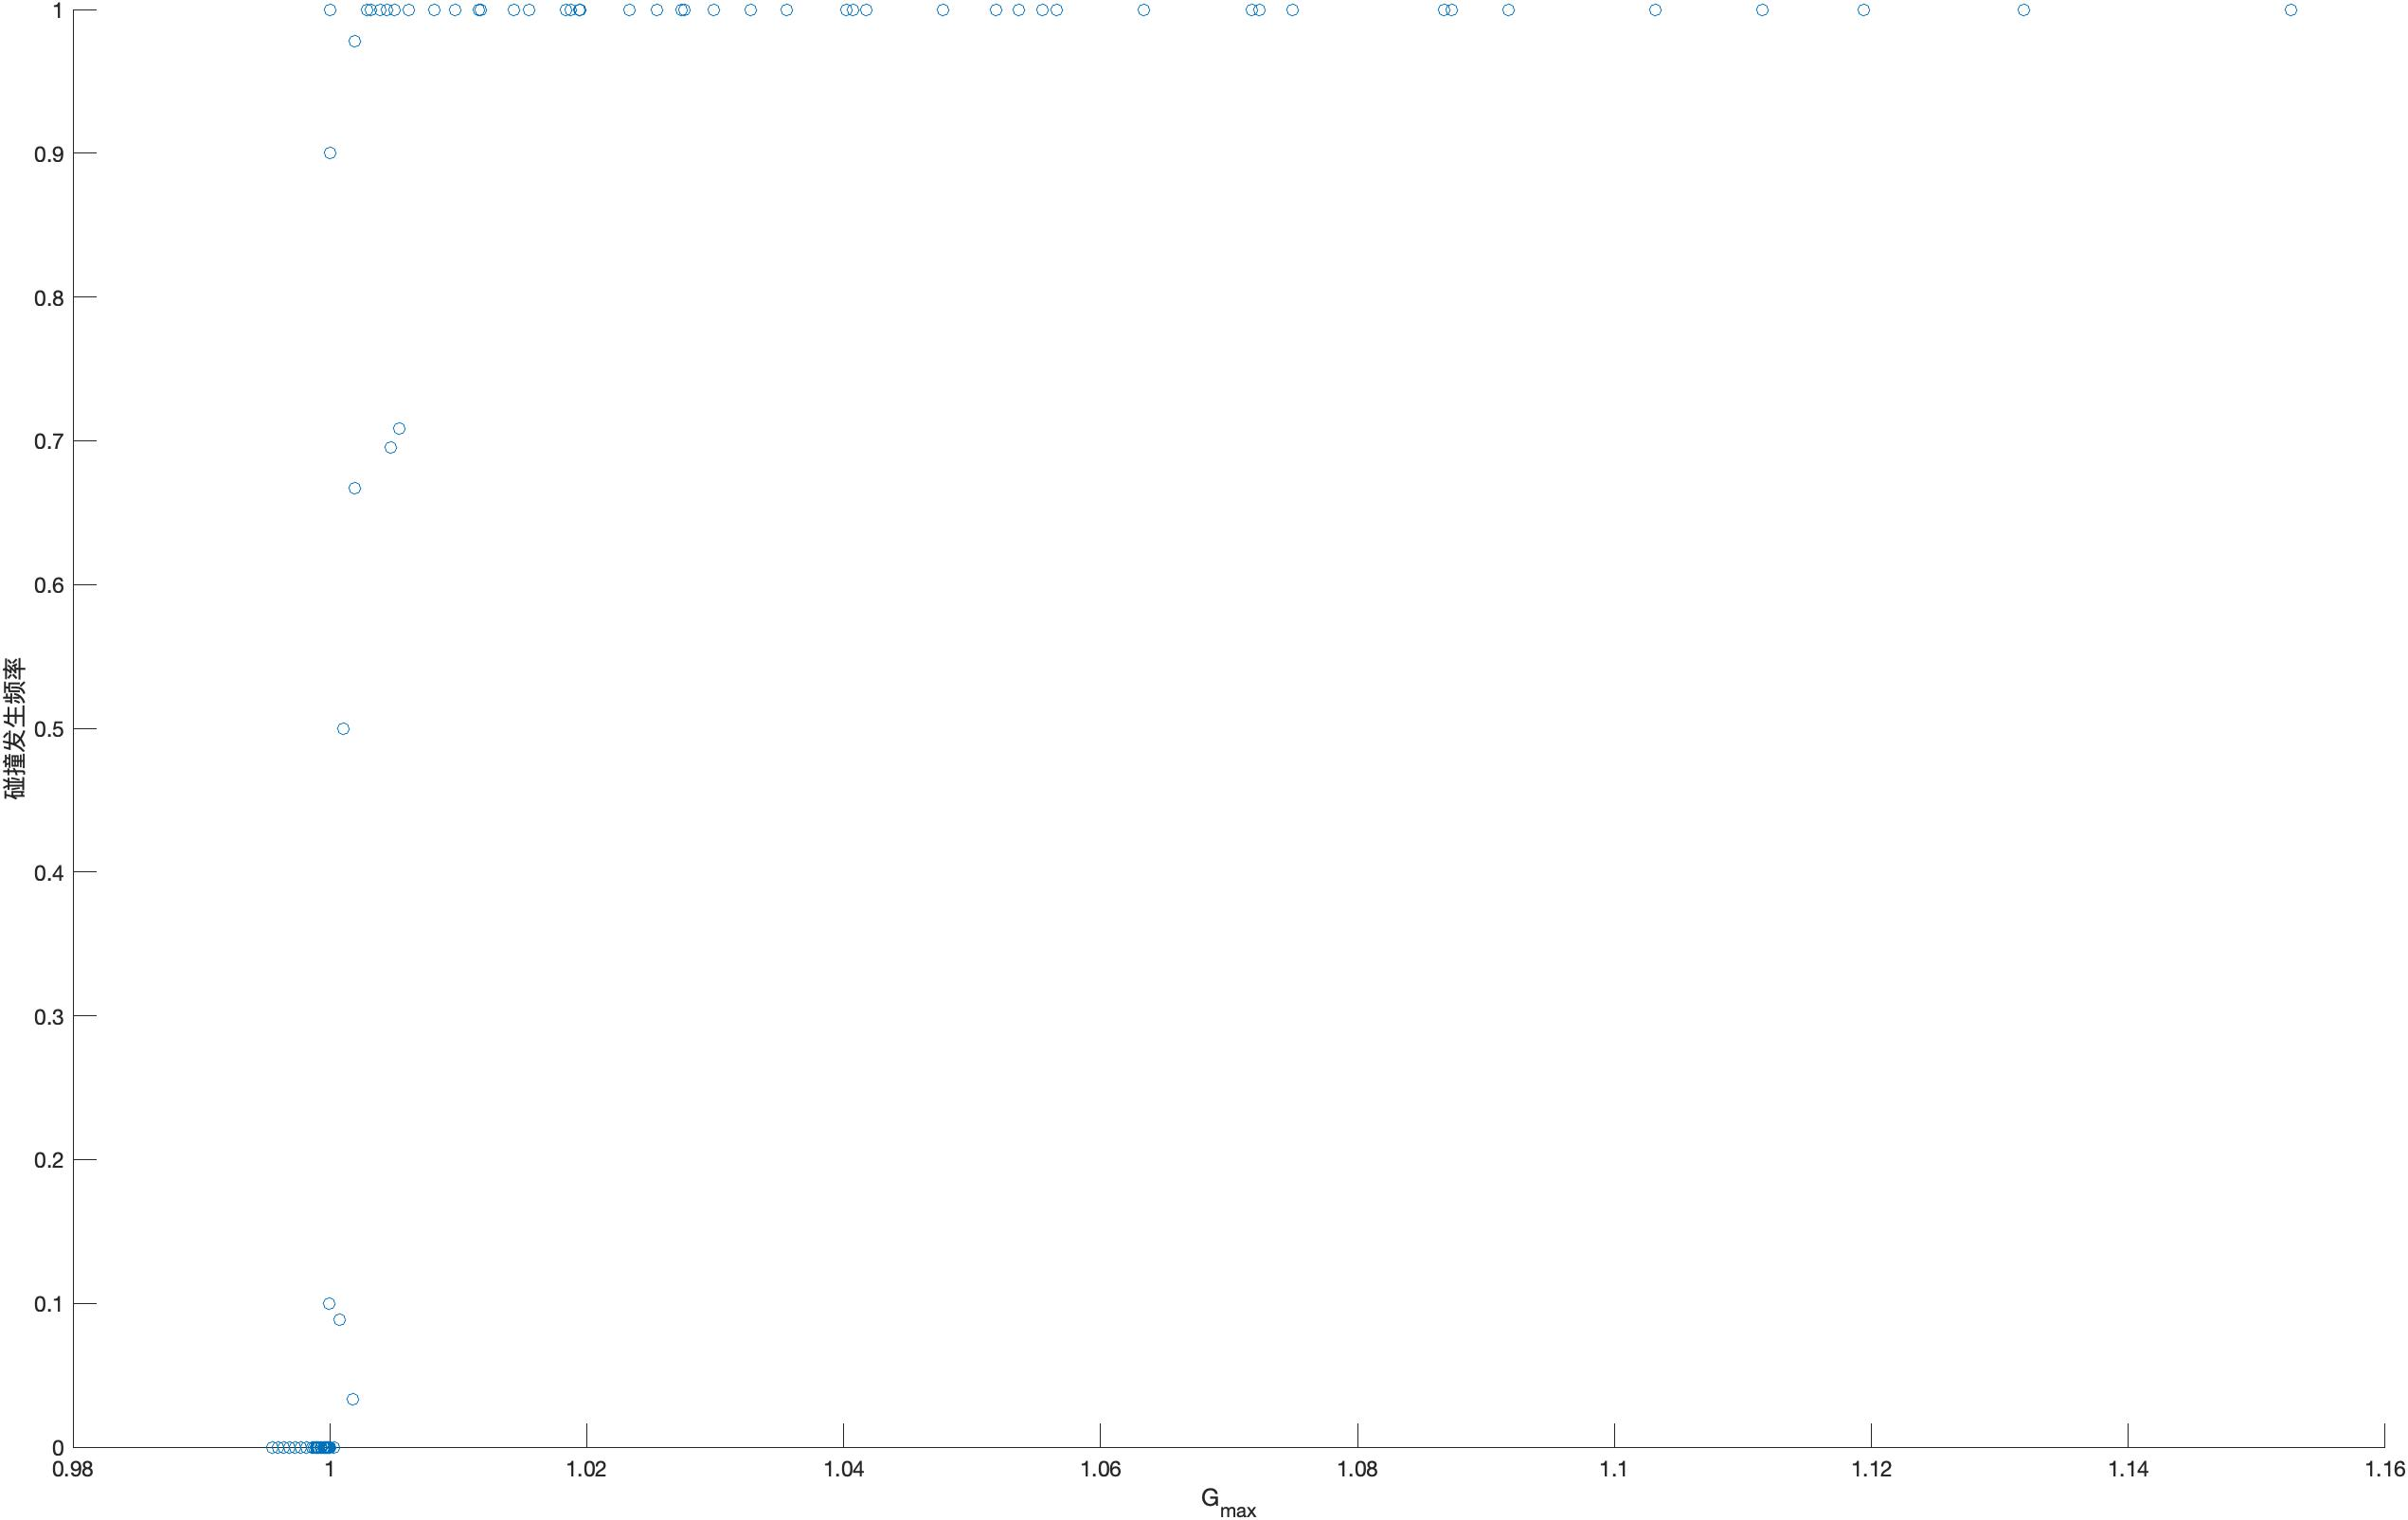
\includegraphics[width=1\linewidth]{chap04-crash-rate.jpg}
    \caption{碰撞频率与稳定性指标$G_{max}$的关系}
    \label{fig:chap04-2}
\end{figure}

实验得到结果如图\ref{fig:chap04-2}所示。可以发现总体上,$G_{max}$越大,碰撞发生的频率也越高,当$G_{max}$足够大时,几乎一定会发生碰撞,当$G_{max}$足够小时,几乎一定不会发生碰撞。
还有一个重要的结论是,理论上队列稳定($G_{max} < 1$)的车队也有可能发生碰撞,而理论上不稳定($G_{max} > 1$)的车队也并不是一定会发生碰撞,即发生碰撞与否并不取决于$G_{max}$的取值,
但与$G_{max}$有一定的关联。

通过图\ref{fig:chap04-2}还可以发现,发生碰撞并不是一个小概率事件,所以将发生碰撞的样本和不发生碰撞的样本分开讨论是有必要的。通过此图像也可以看出,
$G_{max} < 1$的样本多集中在一个较小的区间,而$G_{max} > 1$的样本则比较分散,这与对图\ref{fig:chap04-1}的分析是一致的。

\section{碰撞样本分析}

\subsection{稳定性指标选取}

对于发生了碰撞的样本,其对应的$G_{max}$多是大于1的,$G_{max} > 1$的样本则比较分散,所以用$G_{max}$作为碰撞样本的队列稳定性指标是比较合适的。

\subsection{碰撞风险指标选取}

对于发生了碰撞的样本,有两个衡量车队碰撞风险(安全性)的指标。

一是追尾发生的时间$t_{crash}$,我们认为追尾事故发生得越早,车队整体越不安全。

二是发生追尾的车辆的下标$\mathrm{Index}_{crash}$,我们认为追尾事故发生得越靠近头车,车队整体越不安全。

\subsection{稳定性与碰撞风险关系探究}

首先探究追尾发生的时间$t_{crash}$与车队队列稳定性$G_{max}$之间的关系。与分析是否发生碰撞与车队的稳定性的关系时设计的实验一样,
对自动驾驶车辆比例$p$和初始均衡速度$v_e$进行遍历,挑选出发生了碰撞的样本,计算其对应的$G_{max}$,并统计追尾发生的时间。实验结果如图\ref{fig:chap04-3}所示。

\begin{figure}
    \centering
    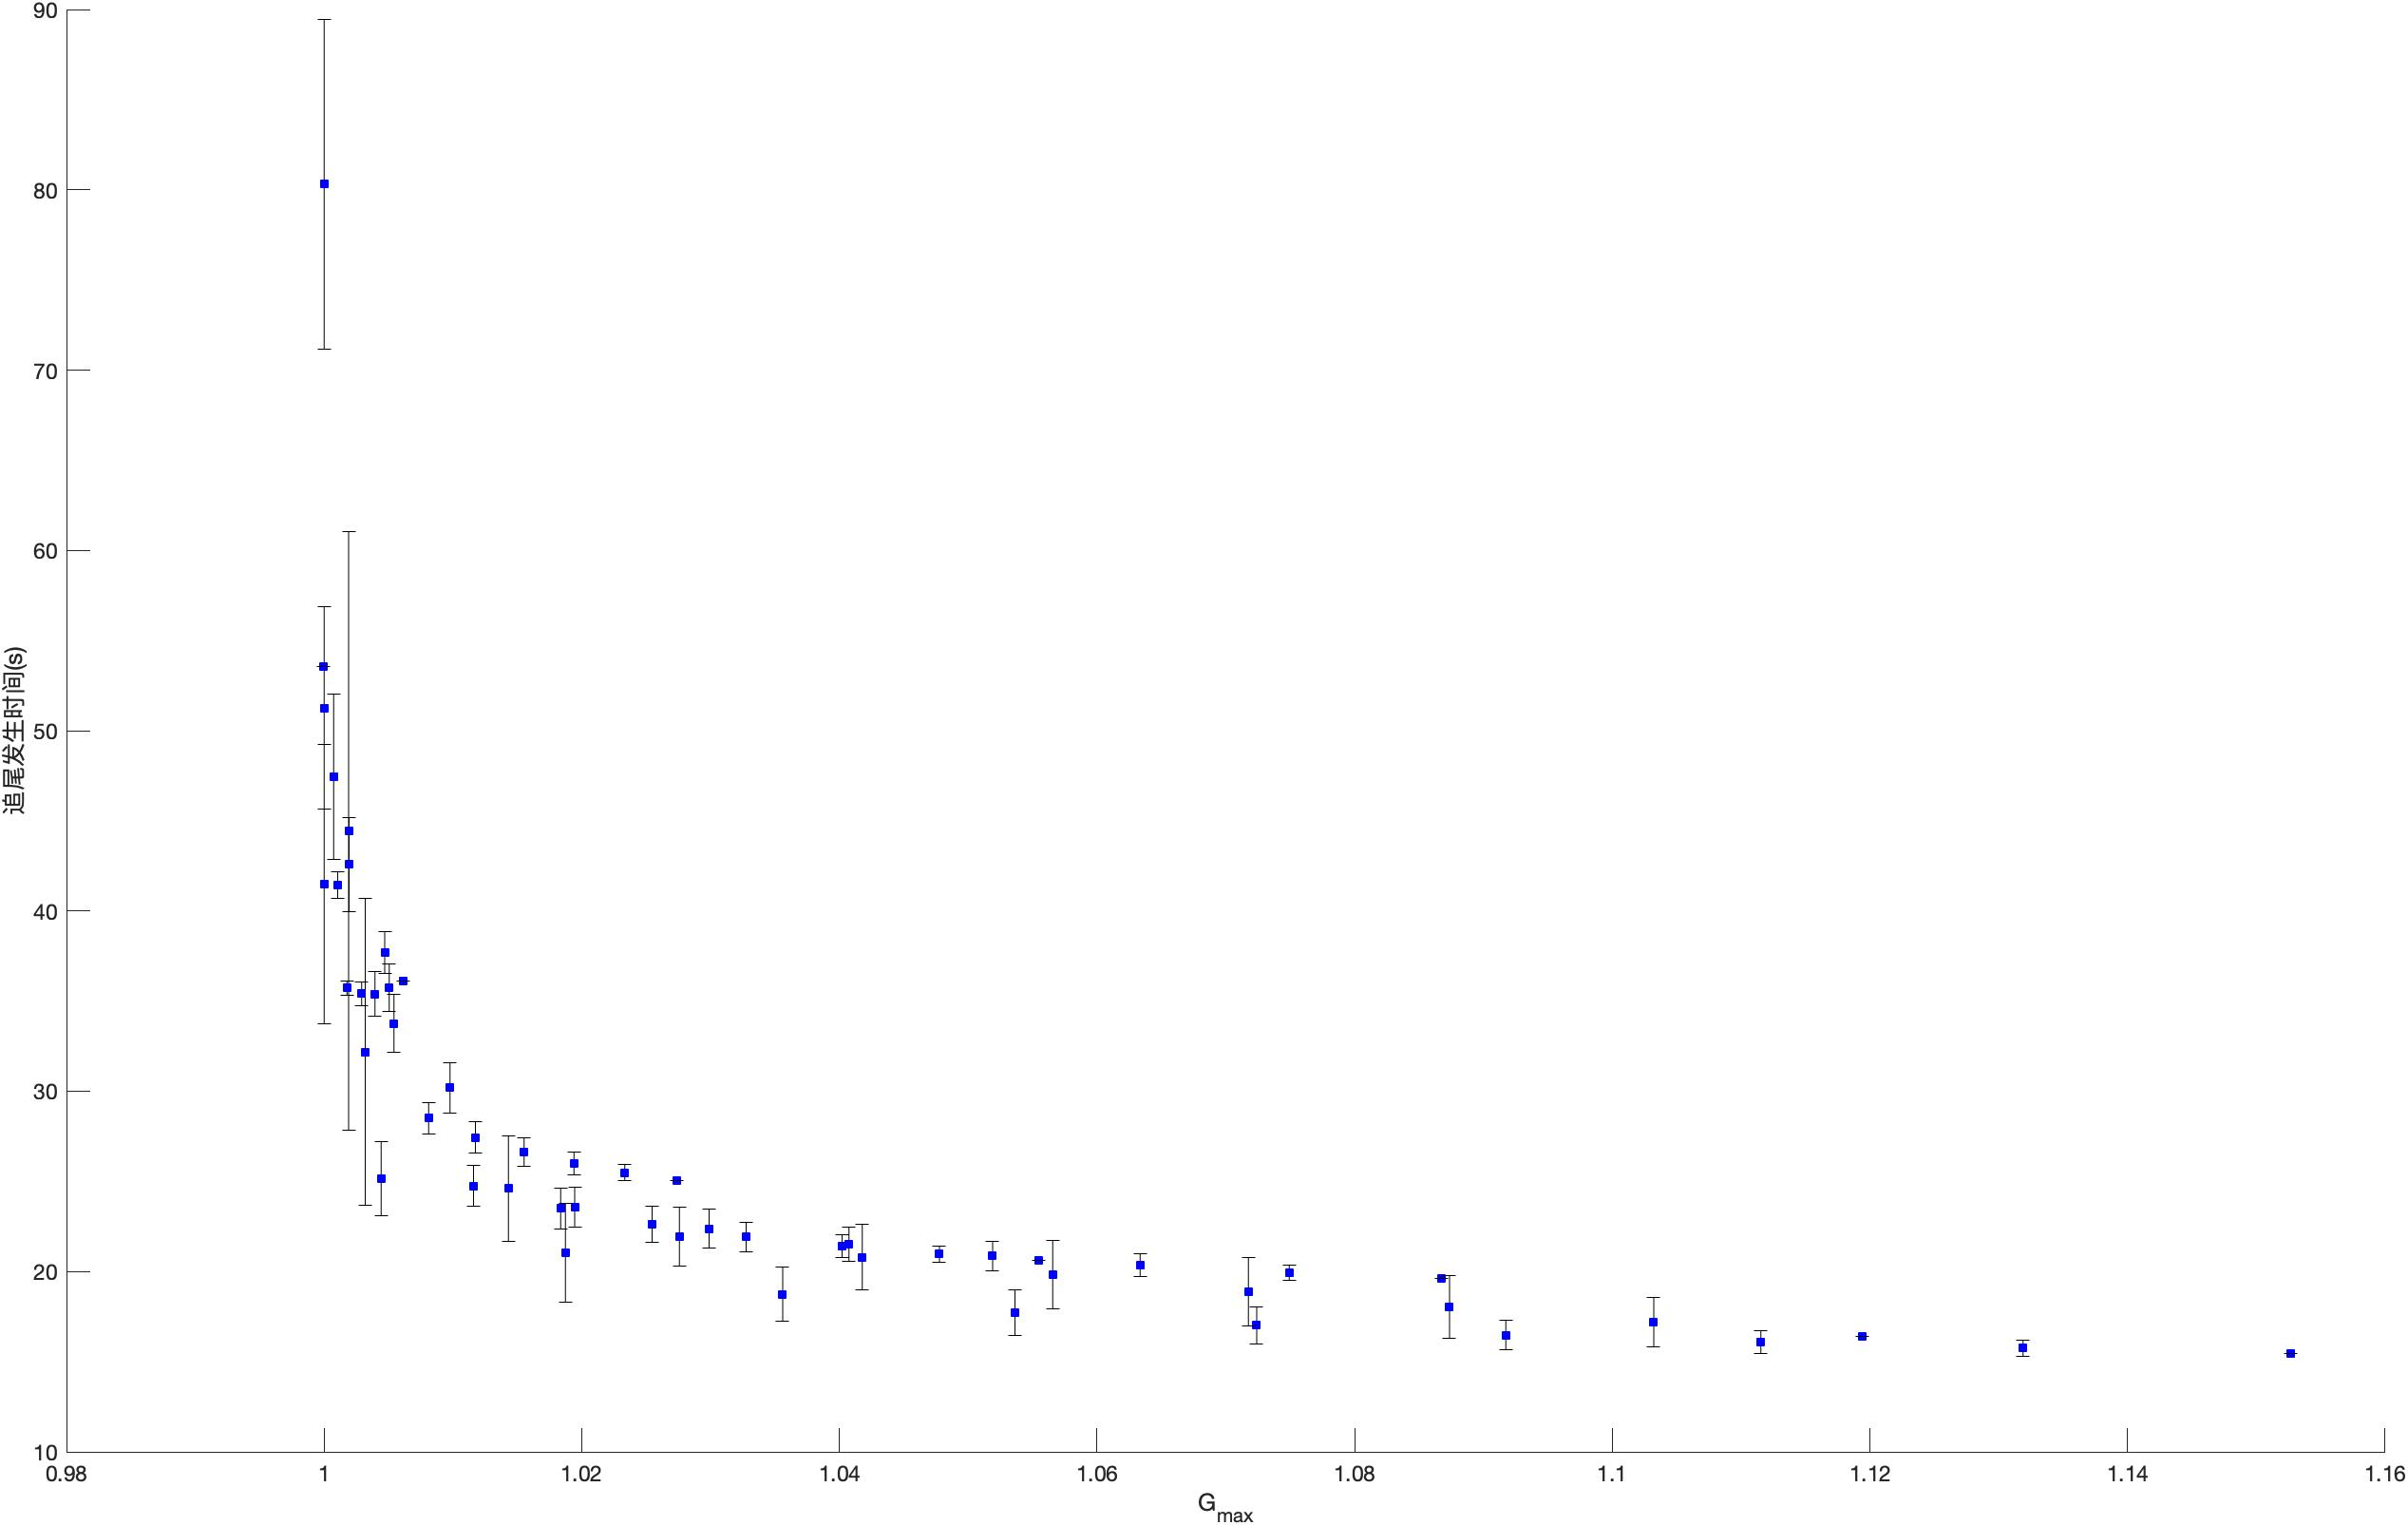
\includegraphics[width=1\linewidth]{chap04-t_crash.jpg}
    \caption*{Error bar代表标准差}
    \caption{追尾发生时间$t_{crash}$与稳定性指标$G_{max}$的关系}
    \label{fig:chap04-3}
\end{figure} 

可以观察到随着$G_{max}$的增大,碰撞发生的时间越小,即车队的队列稳定性越差,追尾发生的越快。其规律类似于反比例函数。此现象可以解释为:$G_{max}$越大,车队的队列稳定性越差,
扰动被放大的速度越快,碰撞就发生得越早。该关系是稳定性与碰撞风险在时间维度上的关系。

而通过发生追尾的车辆的下标$\mathrm{Index}_{crash}$则可以得到稳定性与碰撞风险在空间维度上的关系。如图\ref{fig:chap04-4}所示。

\begin{figure}
    \centering
    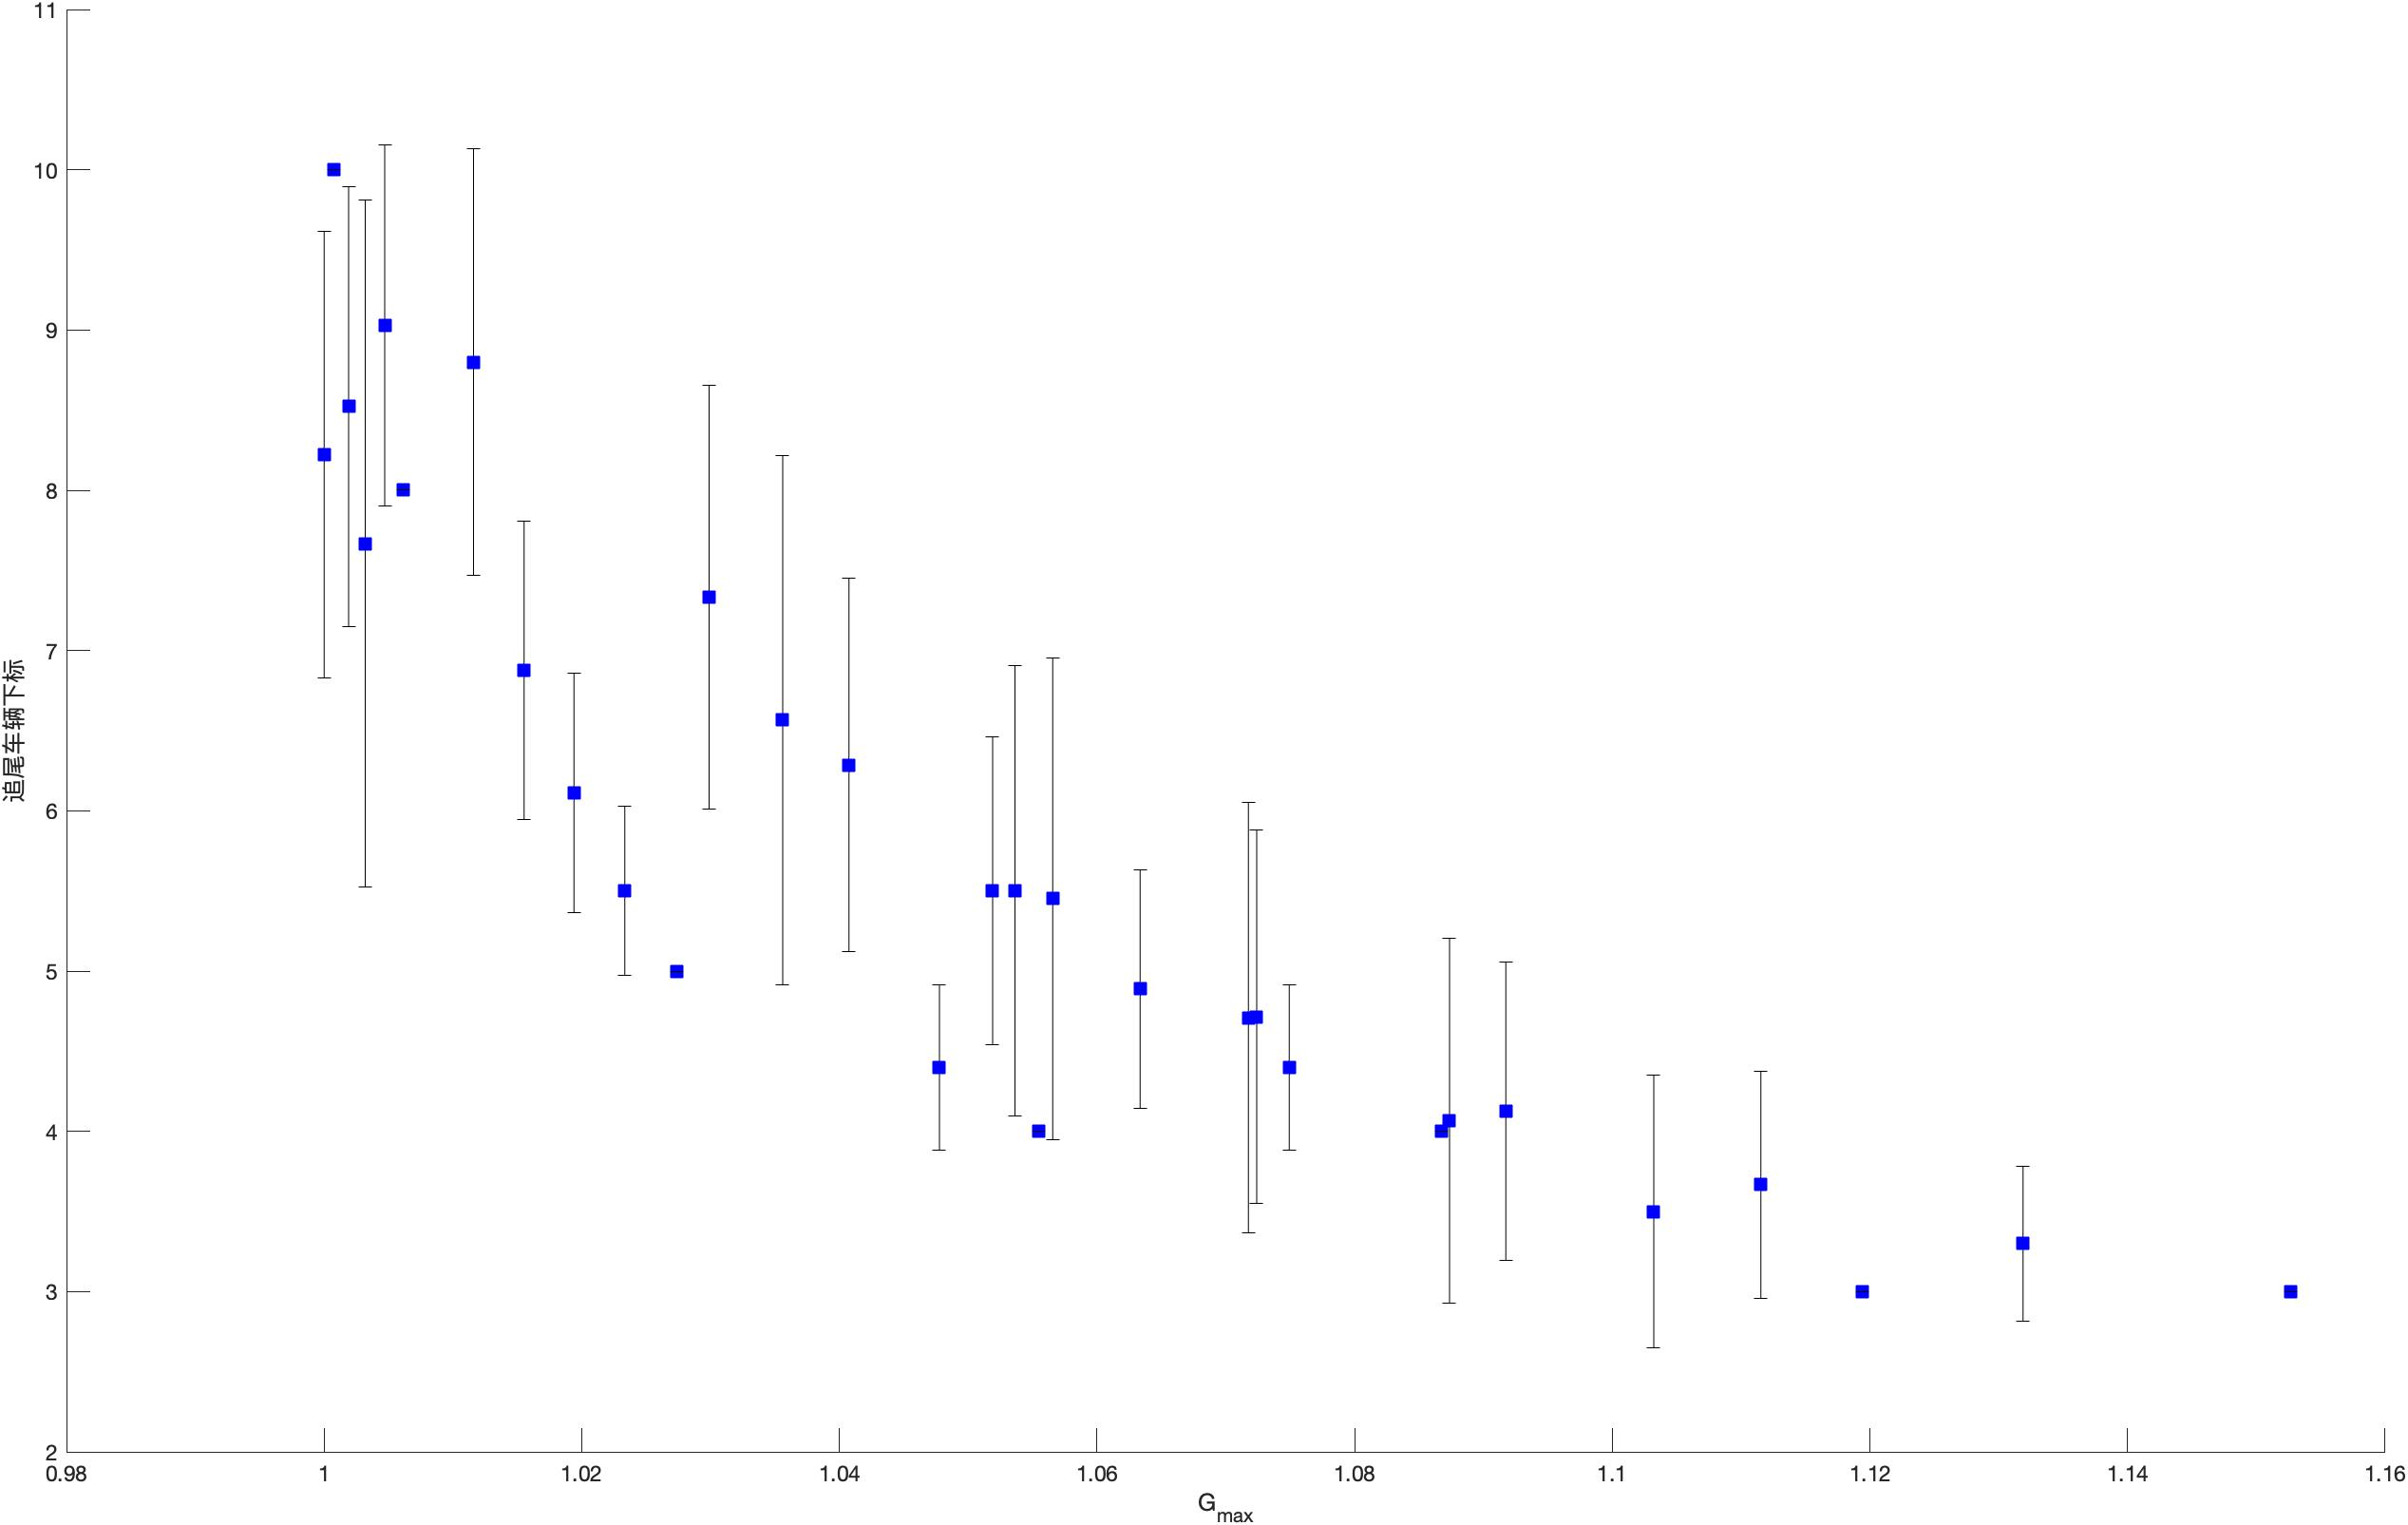
\includegraphics[width=1\linewidth]{chap04-crash_index.jpg}
    \caption*{Error bar代表标准差}
    \caption{追尾车辆下标$\mathrm{Index}_{crash}$与稳定性指标$G_{max}$的关系}
    \label{fig:chap04-4}
\end{figure} 

从图\ref{fig:chap04-4}中可能看出$\mathrm{Index}_{crash}$与$G_{max}$存在相关性。整体来看,$G_{max}$越大,$\mathrm{Index}_{crash}$越小,即车队队列稳定性越差,
碰撞发生得越靠前。这可以解释为:头车受到扰动后,扰动沿着车队传播,传递函数最大增益$G_{max}$越大,稳定性越差,扰动被放大的速度越快,碰撞发生得越靠前。

无论是从指标$t_{crash}$来看,还是从指标$\mathrm{Index}_{crash}$来看,都可以发现,车队的队列稳定性越差,车队的安全性越差。

在车队中,人工驾驶车辆和自动驾驶车辆对扰动的传递情况是不同的。通过\ref{sec:3.3}的仿真可以发现,在理想情况下,自动驾驶车辆会将前车的扰动略微放大,而扰动经过人工驾驶车辆则在不断
衰减;而对于模拟真实场景下的仿真,当给人类驾驶员引入$1.2s$的反应延迟后,似乎人工驾驶车辆也带来了不稳定的因素。下面就通过改变车队中车辆的排列,探究碰撞风险在车队中的演化机理。

\subsection{车队碰撞风险演化机理探究}
\label{sec:4.2.4}

\subsubsection{空间分布指标选取}
\label{sec:4.2.4.1}

参考王大钧在空间分布指标选取方面的工作\cite{wang2021auto},在对自动驾驶车辆在车队中的空间分布研究时,主要关注两个指标。

一是自动驾驶车辆整体靠近头车的程度。该指标的意义在于,如果自动驾驶车辆整体越靠前,那么扰动最先由自动驾驶车辆传递,通过对追尾车辆下标的分析,可以分析发生碰撞的下标与自动驾驶整体分布的下标之间的关系。

二是自动驾驶车辆的分散程度。在指标的意义在于,如果自动驾驶车辆会放大扰动,人工驾驶车辆可以衰减扰动,那么将自动驾驶车辆分散排布在车队中可能会比将自动驾驶车辆集中在一起更加安全。

通过对同一稳定性的不同车辆排列进行仿真实验,可以探究,下面对两个指标的计算方式进行介绍。 \\

\noindent \textbf{(1)队首聚集度}

队首聚集度($\mathrm{Index}_{front}$)衡量了车队中自动驾驶车辆整体靠近头车的程度。记车队中共有$n$辆跟随车辆,其中有$m$辆是自动驾驶车辆,每一辆自动驾驶车辆在车队中的下标为$C = (c_1, c_2, \cdots, c_m)$,同时记$C(i) = c_i$,
那么队首聚集度的计算公式为

\begin{equation}
    \begin{cases}
      temp = \frac{\sum_{i=1}^{m}[C(i) - 1 ]}{nm - \sum_{i=1}^{m}i} \\
      \mathrm{Index}_{front} = \frac{temp - \min(temp)}{\max(temp) - \min(temp)}
    \end{cases}
    \label{eq:chap04-2}
\end{equation}

在式(\ref{eq:chap04-2})中进行了归一化,指标值域为$[0,1]$,
且指标取值与自动驾驶车辆整体靠近头车的程度是正相关的。为了使该指标有意义,车队中应当至少包含1辆自动驾驶车辆。 \\

\noindent \textbf{(2)分散均匀度}

分散均匀度($\mathrm{Index}_{disp}$)衡量了车队中自动驾驶车队整体的分散程度。关于车队的描述与队中聚集度相同,分散均匀度的计算方式为

\begin{equation}
    \begin{cases}
      temp = \frac{\sum_{i=1}^m [C(i)-C(i-1)]^{-1}}{m-1} \\
      \mathrm{Index}_{disp} = \frac{temp - \min(temp)}{\max(temp) - \min(temp)}
    \end{cases}
    \label{eq:chap04-3}
\end{equation}

同样,在式(\ref{eq:chap04-3})中也进行了归一化,指标值域为$[0,1]$,且指标取值越小说明说明自动驾驶车辆总体分布越分散、越均匀。在使用该指标时,需要车队中至少有2辆跟驰车辆。

\subsubsection{仿真实验结果分析}

实验设计如下:固定自动驾驶车辆比例$p=0.5$,初始均衡速度$v_e = 15m/s$。通过计算可以发现该取值下车队理论上是队列不稳定的,通过图\ref{fig:chap04-2}可以看出在该稳定性下车队非常容易发生碰撞。
实验的其他设置与前文中的实验保持一致。

实验结果如图\ref{fig:chap04-5}所示。

\begin{figure}
    \centering
    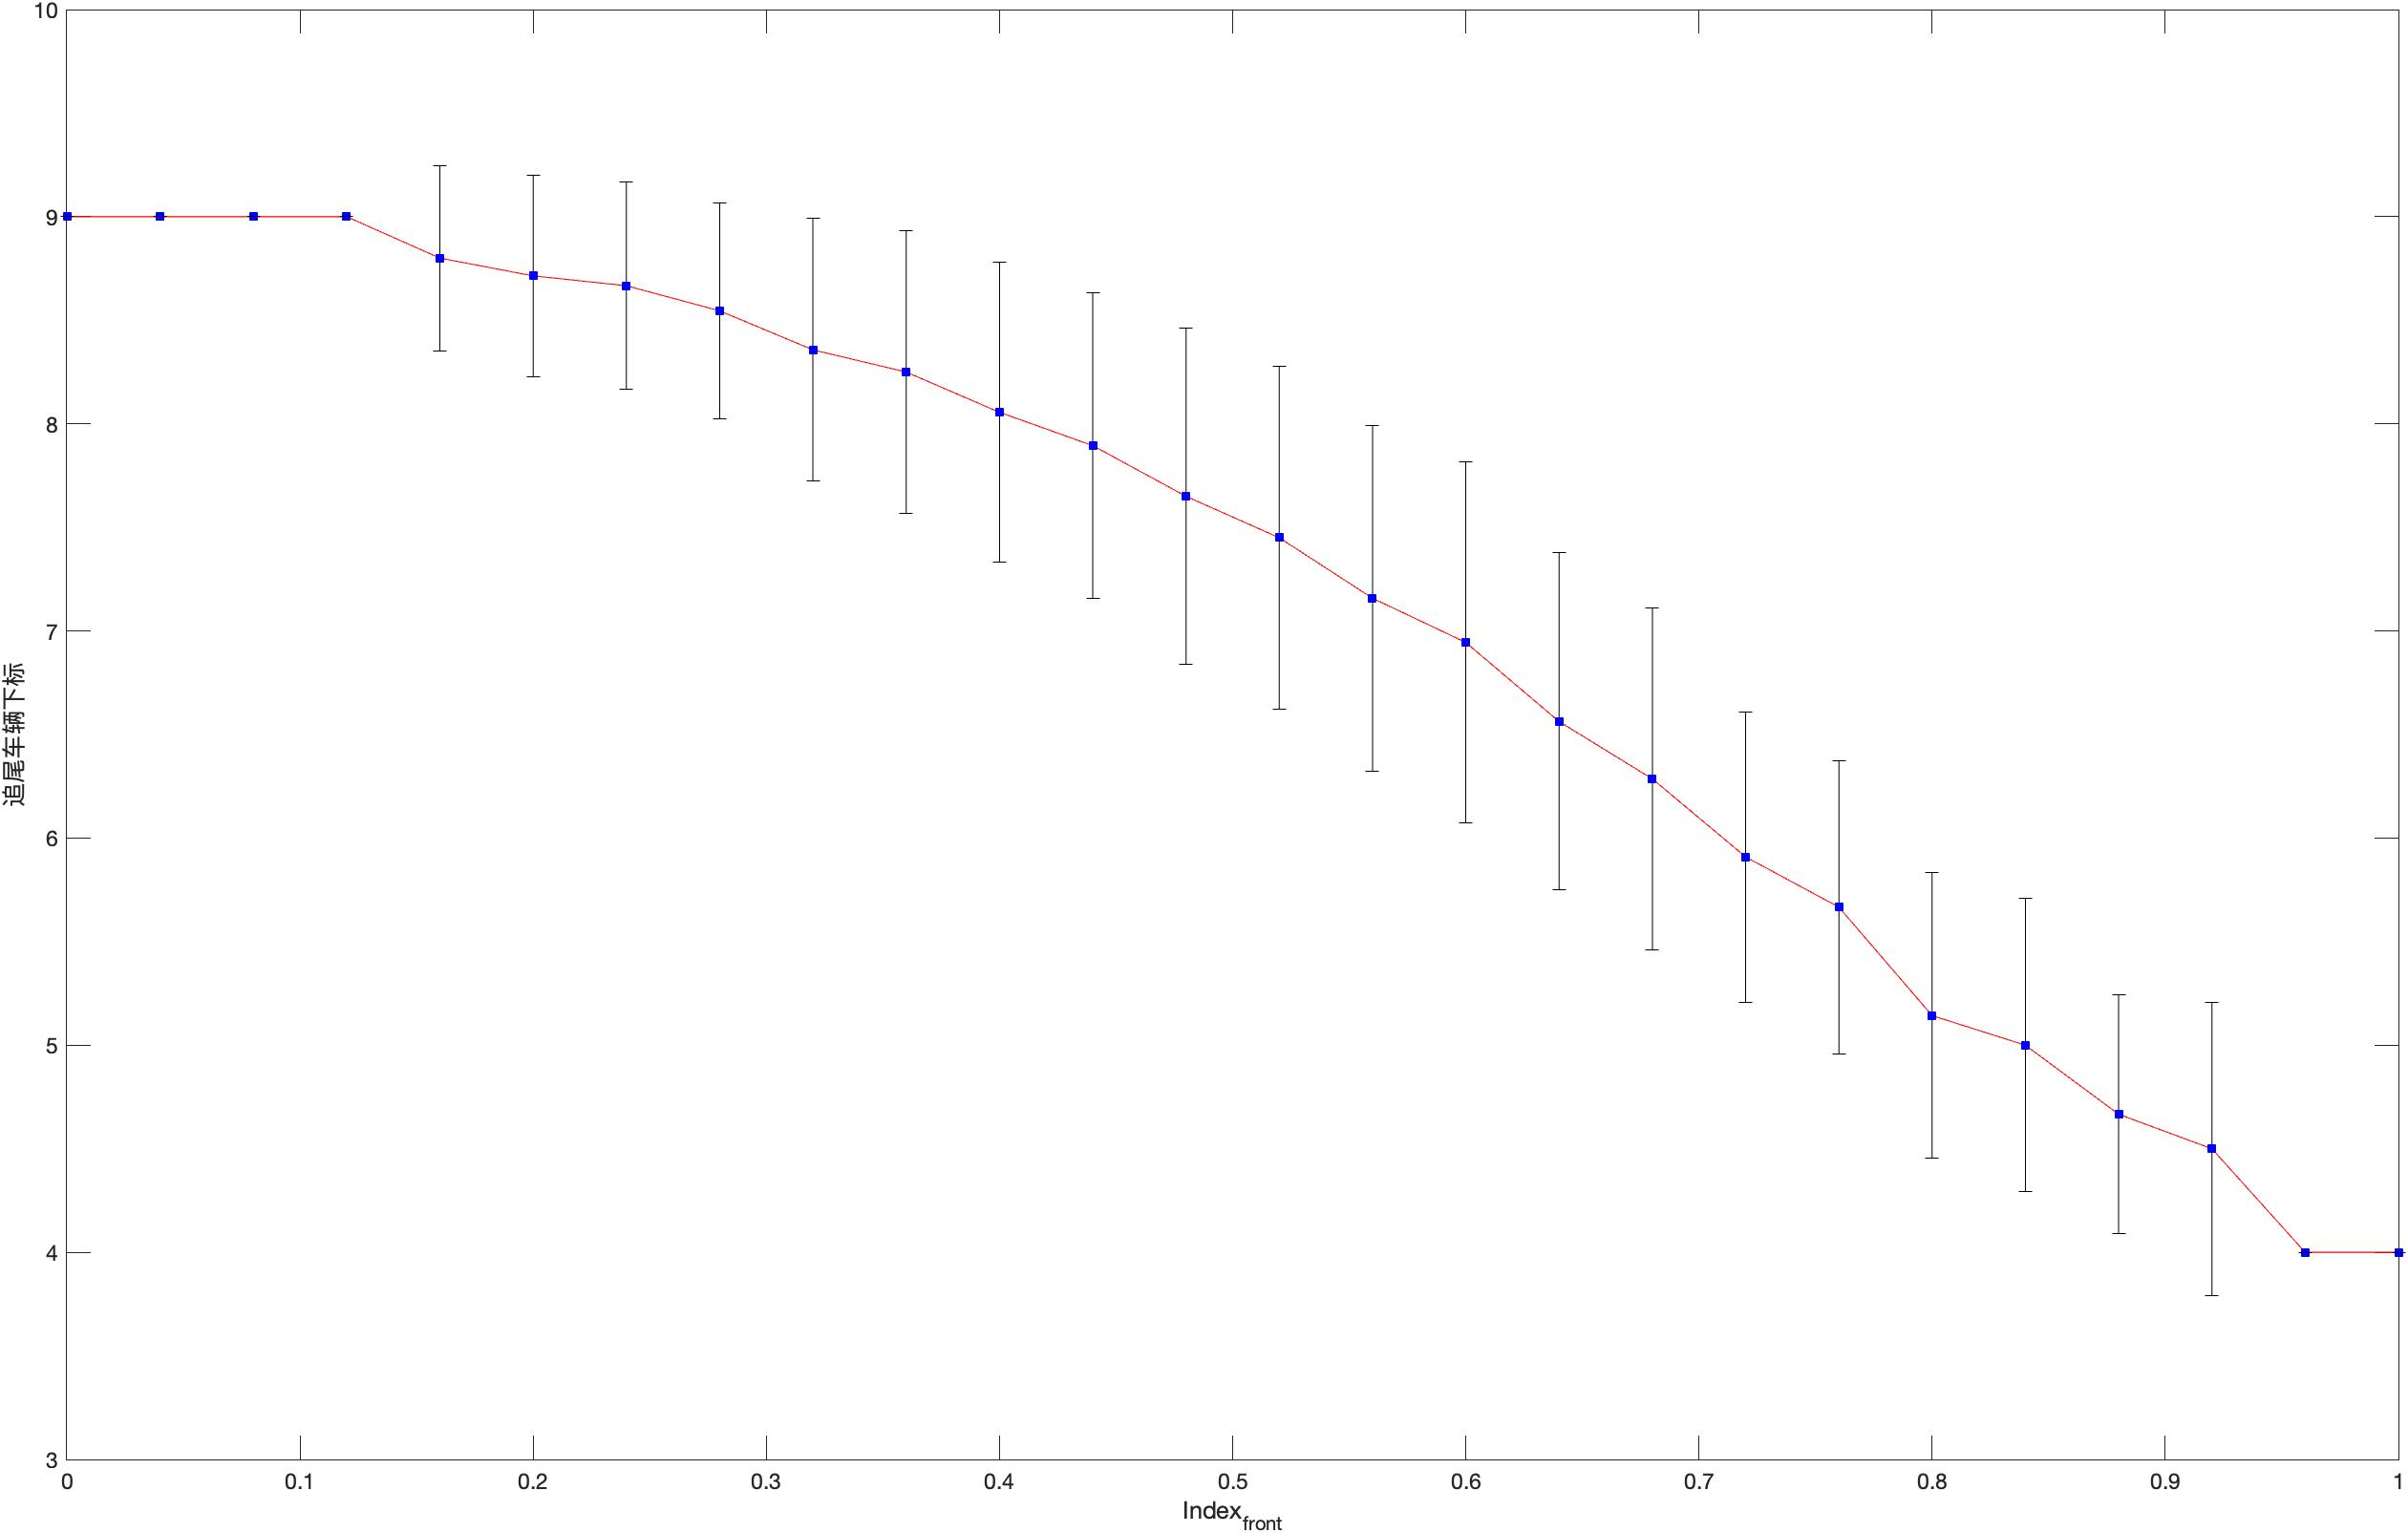
\includegraphics[width=1\linewidth]{chap04-front-crash.jpg}
    \caption*{Error bar代表标准差}
    \caption{队首聚集度与追尾车辆下标的关系}
    \label{fig:chap04-5}
\end{figure} 

可以看出队首聚集度与追尾车辆的下标是负相关的,且存在一定的线性关系。计算二者的Pearson相关系数为$-0.8281$,对于向量$\mathrm{X}$和向量$\mathrm{Y}$,其Pearson相关系数的计算公式如式(\ref{eq:chap04-4})。

\begin{equation}
    r = \frac{\mathbb{E}\mathrm{XY}-\mathbb{E}\mathrm{X}\mathbb{E}\mathrm{Y}}{\sqrt{\mathbb{E}\mathrm{X^2}-(\mathbb{E}\mathrm{X})^2}\sqrt{\mathbb{E}\mathrm{Y^2}-(\mathbb{E}\mathrm{Y})^2}}
    \label{eq:chap04-4}
\end{equation}

从图\ref{fig:chap04-5}可以看出,当队首聚集度指标$\mathrm{Index}_{front}$越大,追尾车辆下标越小,即自动驾驶车辆整体越远离头车,追尾发生在越靠近头车的地方,即追尾总是倾向于发生在人工驾驶车辆处。这也可以说明人工驾驶车辆会给车队带来更大的碰撞风险。

为了获得更加清晰的碰撞风险演化机理,将自动驾驶车辆比例$p$以0.1的步长遍历0到1,对于每一个$p$的取值,初始均衡速度以$2m/s$的步长遍历$10m/s$
到$30m/s$,对实验中追尾车辆及其前后车的车辆种类进行了统计,结果如表\ref{tab:chap04-2}所示。

\begin{table}
    \centering
    \caption{追尾车辆及其前后车车辆种类统计}
    \begin{tabular}{ccl}
      \toprule
      追尾车辆类型                 &                                &  数量及比例  \\
      \midrule
      \multirow{4}{*}{AV : 999 (19.09\%)}         &    \multirow{2}{*}{前车类型}    &   AV : 47 (4.70 \%)    \\
                                 &                                       &   HV : 952 (95.30 \%)   \\
      \cline{2-3}
                                 &    \multirow{2}{*}{后车类型$^*$}    &   AV : 508 (50.58 \%)    \\
                                 &                                &   HV : 247 (24.72 \%)   \\       
      \hline
      \multirow{4}{*}{HV : 4235 (80.91\%)}        &    \multirow{2}{*}{前车类型}    &   AV : 1753 (41.39 \%)    \\
                                 &                                &   HV : 2482 (58.61 \%)  \\      
      \cline{2-3}
                                 &    \multirow{2}{*}{后车类型$^*$}    &   AV :1948 (46.00 \%)  \\
                                 &                                &   HV : 2245 (53.01 \%)  \\     
      \bottomrule
    \end{tabular}
    \caption*{*由于有部分追尾车辆已是尾车,所以后车类型会出现比例和小于1的情况}
    \label{tab:chap04-2}
  \end{table}

可以发现追尾车辆大多是人工驾驶车辆造成的,占到了$80.91\%$,这与图\ref{fig:chap04-5}呈现的追尾总是倾向于发生在人工驾驶车辆处的规律是吻合的。通过观看可视化的仿真过程,发现人工驾驶的追尾多是由于人工驾驶车辆减速不及时造成的,造成这一现象的一个原因可能是在仿真时给人工驾驶员设置了$1.2s$的反应延迟,另一个可能原因是扰动在人工驾驶车辆传递过程中衰减的速度较慢,即相比自动驾驶车辆,人工驾驶车辆很有效地抵抗扰动,造成了较大的碰撞风险。

对被追尾车辆(即表中的前车)的类型进行分析,无论是人工驾驶车辆,还是自动驾驶车辆,其追尾的多是人工驾驶车辆,这一现象对于自动驾驶车辆更为明显,人工驾驶车辆占到自动驾驶车辆追尾车辆的$95.30\%$,这更能说明人工驾驶车辆对扰动的抵抗能力不是很强,当自动驾驶车辆跟驰自动驾驶车辆时,碰撞风险会变得更大,也很容易发生追尾事故。同时表中也列出了追尾车辆后车的类型,但由于无论是人工驾驶车辆,还是自动驾驶车辆,其跟驰模型都没有考虑后车,所以此处就不分析后车类型的分布情况了。

同时,也统计了队首聚集度与追尾发生时间之间的关系,如图\ref{fig:chap04-6}所示。可以发现二者也有很好的线性关系,其Pearson相关系数为$-0.7950$。队首聚集度越大,自动驾驶车辆整体越远离头车,扰动首先由人工驾驶车辆传递,由于人工驾驶车辆会引入更大的碰撞风险,所以碰撞也会更早地发生。

\begin{figure}
    \centering
    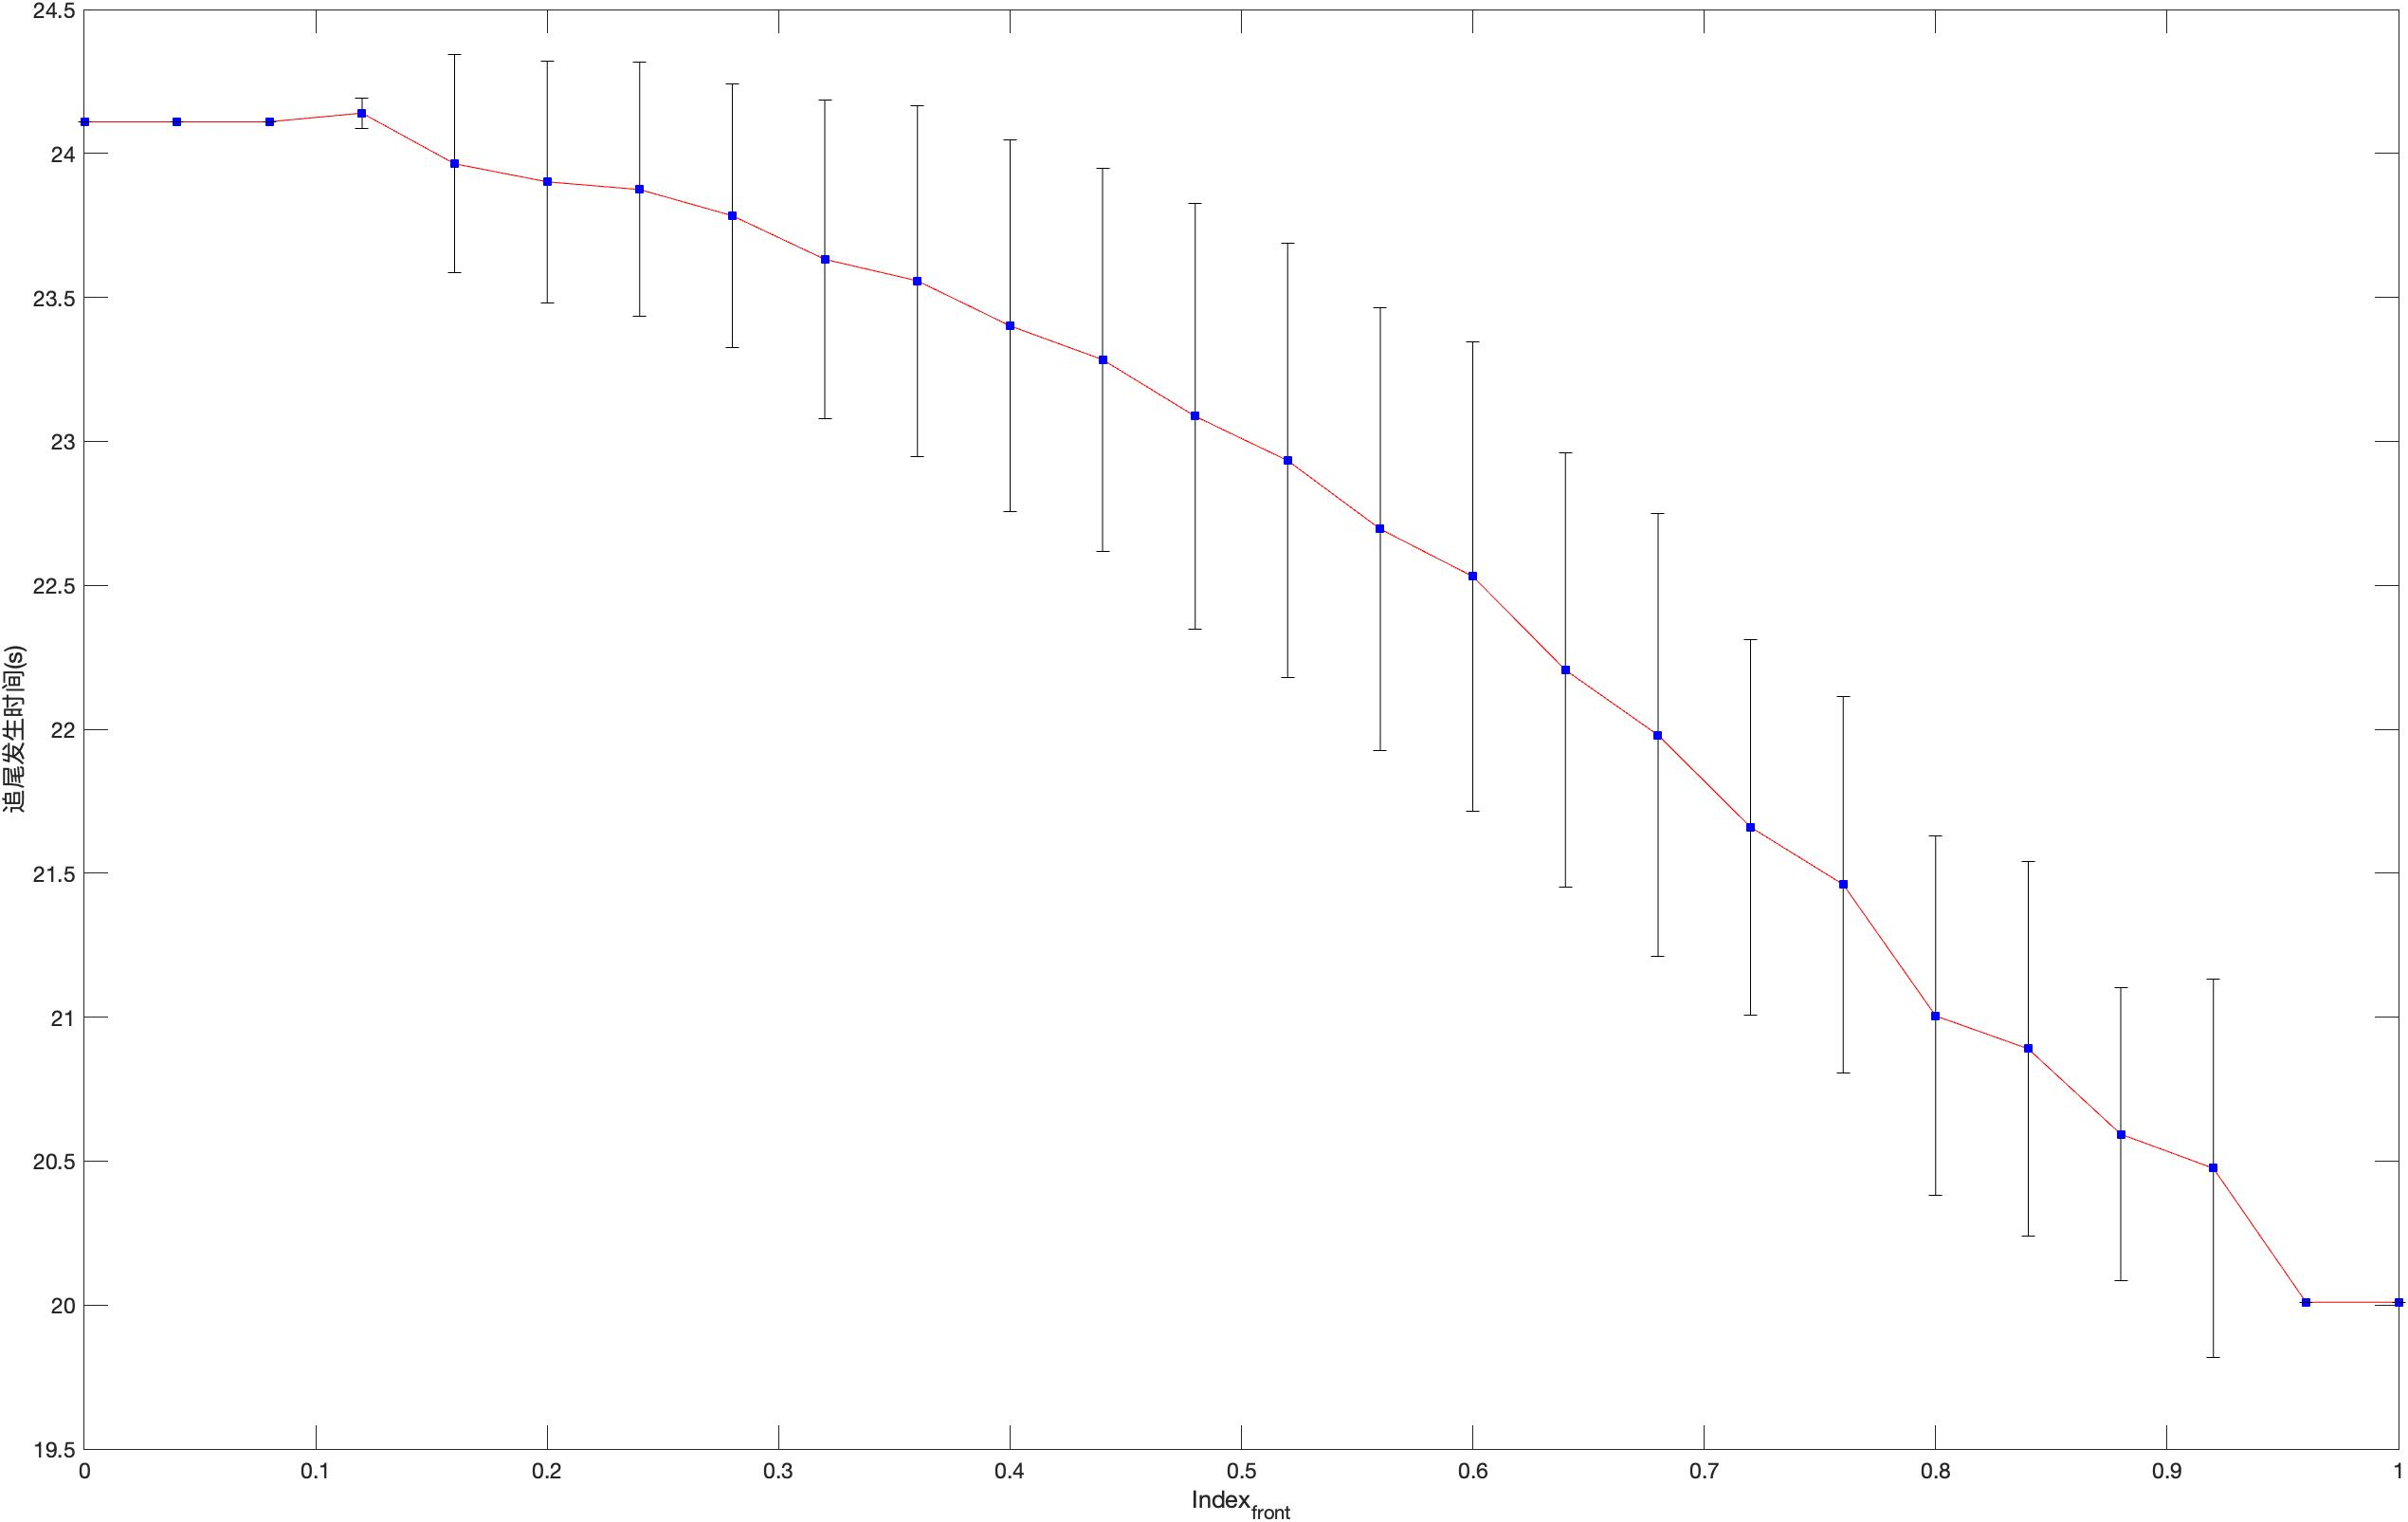
\includegraphics[width=1\linewidth]{chap04-front-time.jpg}
    \caption*{Error bar代表标准差}
    \caption{队首聚集度与追尾发生时间的关系}
    \label{fig:chap04-6}
\end{figure} 

另一个空间分布指标是分散均匀度,与分析队首聚集度时设计的实验相同,这里也固定人工驾驶车辆比例为$0.5$,初始均衡速度为$15m/s$,统计实验过程中追尾的下标与发生的时间,结果如图\ref{fig:chap04-7}所示。

\begin{figure}
    \centering
    \subcaptionbox{分散均匀度与追尾发生时间的关系 \label{fig:chap04-7-1}}
      {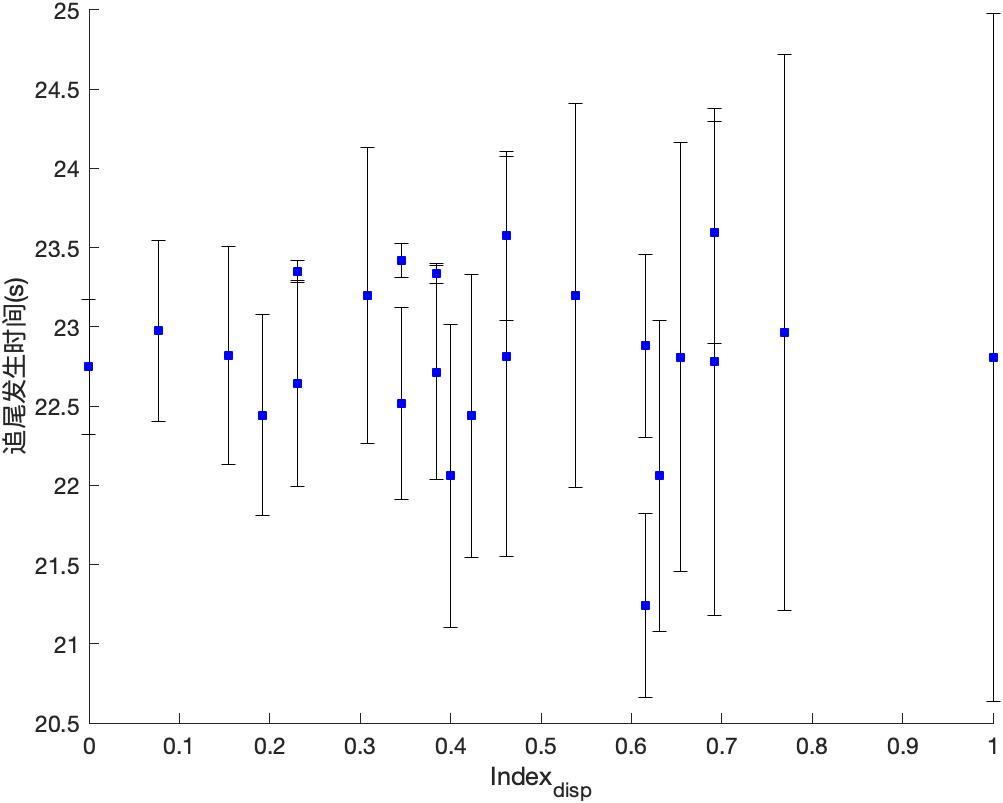
\includegraphics[width=0.49\linewidth]{chap04-disp-time.jpg}}
    \subcaptionbox{分散均匀度与追尾车辆下标的关系 \label{fig:chap04-7-2}}
      {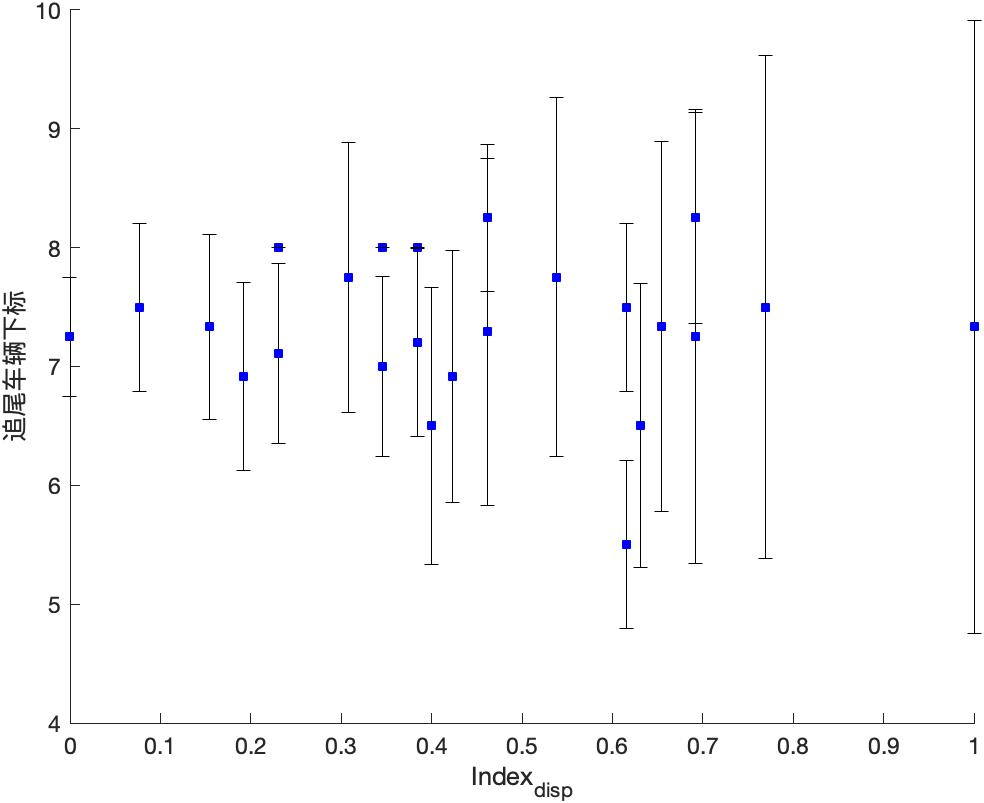
\includegraphics[width=0.49\linewidth]{chap04-disp-index.jpg}}
      \caption{分散均匀度与碰撞风险关系分析}
    \label{fig:chap04-7}
  \end{figure}

可以发现分散均匀度与追尾车辆下标以及追尾发生时间均没有明显关系,这说明自动驾驶车辆在车队中的分散程度并不会影响车队的碰撞风险大小。

\section{非碰撞样本分析}
\label{sec:4.3}

\subsection{稳定性指标选取}

 与碰撞的样本不同,非碰撞的样本大多是理论上队列稳定的样本。由之前的分析得到,稳定样本的车队传递函数无穷范数$G_{max}$集中在一个很小的区间内,区分度不大,所以不适合用$G_{max}$作为非碰撞样本的队列稳定性指标。

 一个衡量一个系统稳定程度常用的指标是该系统受到扰动后,恢复到稳态所需要的时间,我们可以将该概念运用到对非碰撞样本队列稳定性的描述上。我们将从车队受到扰动开始,到车队中每一辆车都恢复到初始均衡速度的$\pm 5\%$范围内为止(并且从此之后各车的速度都保持在均衡速度的$\pm 5\%$以内)的时间称为车队的恢复时间,记作$t_{stable}$。$t_{stable}$越大,车队就越不稳定;反之,车队越稳定。

 值得说明的是,对于虽然没有发生碰撞,但在仿真的$500s$时间内没有达到稳定的样本,用$t_{stable}$这一指标并没有意义,通过统计发现这样的样本是极少数,所以在这一小节中,主要对没有发生碰撞,且在仿真的$500s$恢复的稳态的样本进行分析。

\subsection{碰撞风险指标选取}

由于研究的对象是没有发生碰撞的样本,所以用潜在危险时间(Potential Dangerous Time, PDT)比例来描述车队的碰撞风险。是否存在潜在危险的判断依据如式(\ref{eq:chap04-5})所示。

\begin{equation}
    \increment{x_n} \geqslant A + B - (C - l_{n-1})
    \label{eq:chap04-5}
\end{equation}
其中各变量参数如表\ref{tab:chap01-9}所示。

在仿真的$500s$中,存在潜在危险的时间占总时间的比例称为潜在危险时间比例。

\subsection{稳定性与碰撞风险关系探究}

仿真实验设计如下:以$0.1$的步长对自动驾驶车辆比例$p$进行遍历,对于每一个自动驾驶车辆比例,再以$2m/s$的步长对初始均衡速度进行遍历,将每一次仿真时间的结果进行统计。

图\ref{fig:chap04-8}所示是队列稳定性指标$t_{stable}$与潜在危险时间比例之间的关系。

\begin{figure}
    \centering
    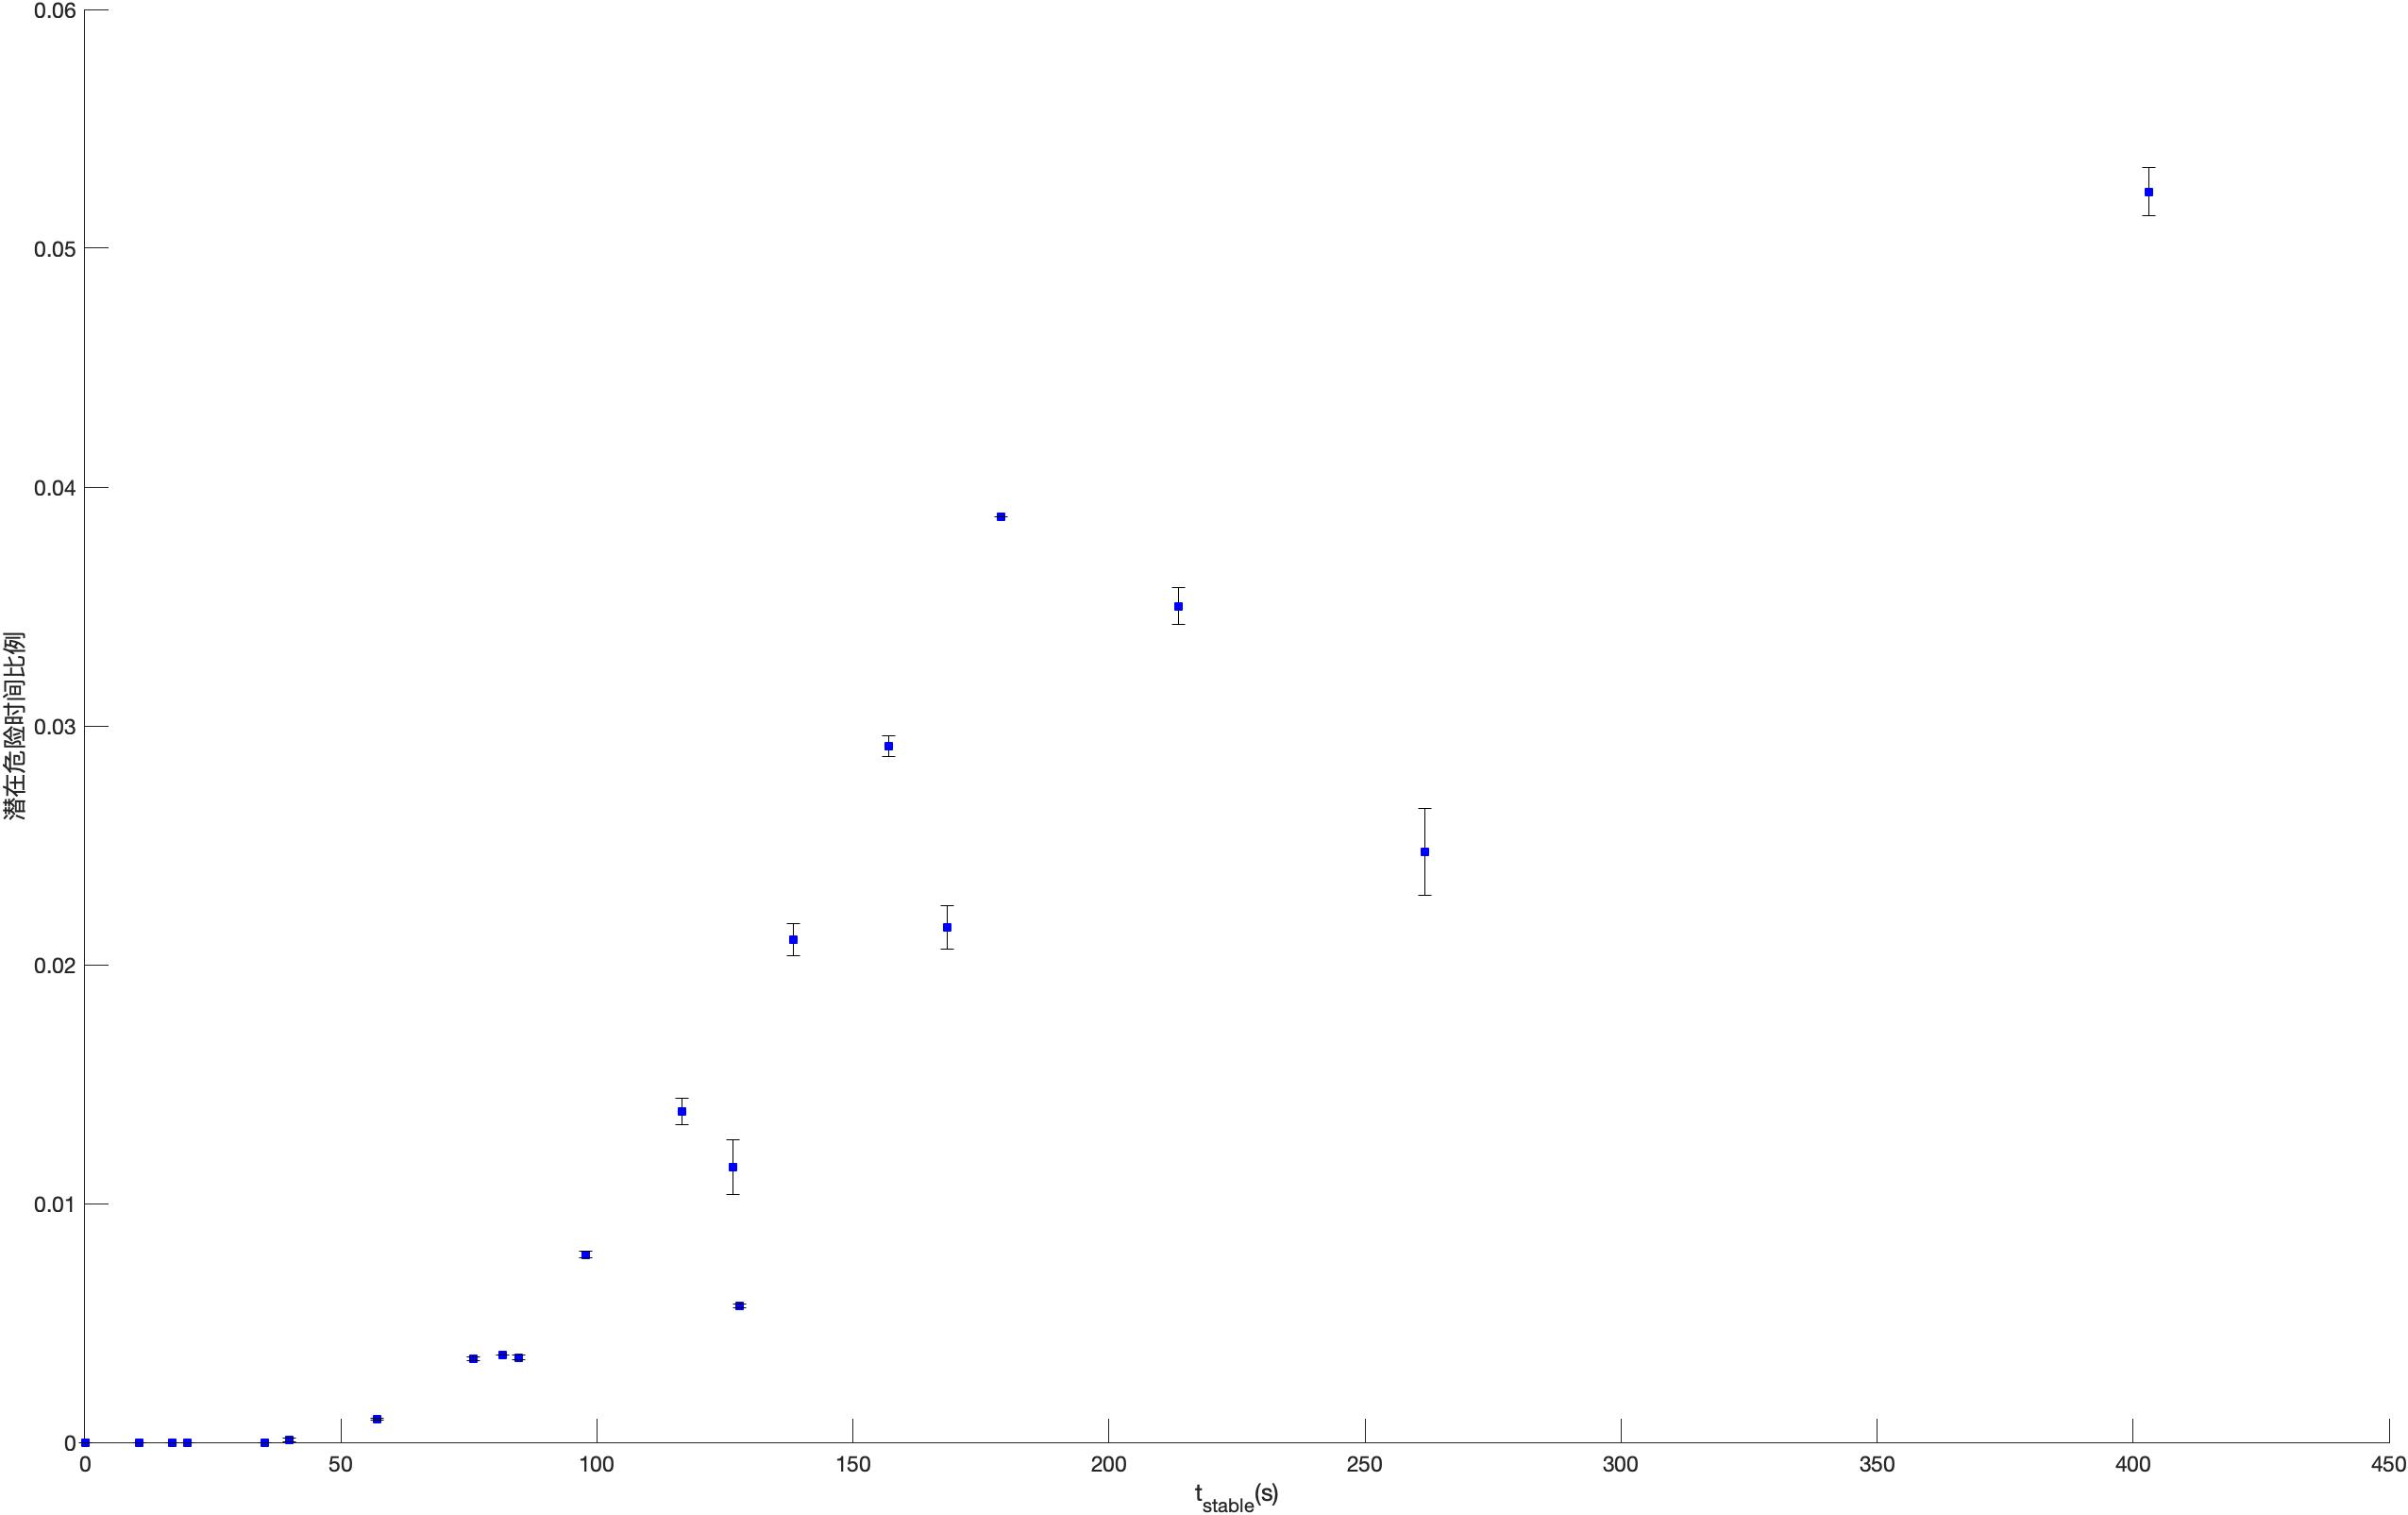
\includegraphics[width=1\linewidth]{chap04-PDT-tstable.jpg}
    \caption*{Error bar代表标准差}
    \caption{潜在危险时间比例与稳定时间的关系曲线}
    \label{fig:chap04-8}
\end{figure} 

可以发现潜在危险时间比例与稳定时间存在明显的相关性,稳定时间$t_{stable}$越小,车队的队列稳定性越好,车队中存在的潜在危险也越少。

在$t_{stable}$较小时(比如小于$50s$),车队能够迅速恢复稳定,此时车队中几乎不存在潜在危险,扰动给车队带来的影响较小;当$t_{stable}$较大时(比如大于$50s$),随着$t_{stable}$的增大,潜在危险时间比例也会增大,二者的Pearson相关系数达到了0.9476,说明二者有很强的相关性,并且可以观察到标准差比较小。

\subsection{车队碰撞风险演化机理研究}

在\ref{sec:4.2.4}中,探究了车队中发生了碰撞的情况下,车队中碰撞风险的演化机理,在\ref{sec:4.2.4.1}中,介绍了2个车队的空间分布指标。接下来将通过这2个指标,探究在车队未发生碰撞的情况下,车队中碰撞风险的演化机理。

给定车队中自动驾驶车辆比例为$0.5$,初始均衡速度为$20m/2$,图\ref{fig:chap04-9}所示是潜在危险时间比例与队首聚集度的关系。

\begin{figure}
    \centering
    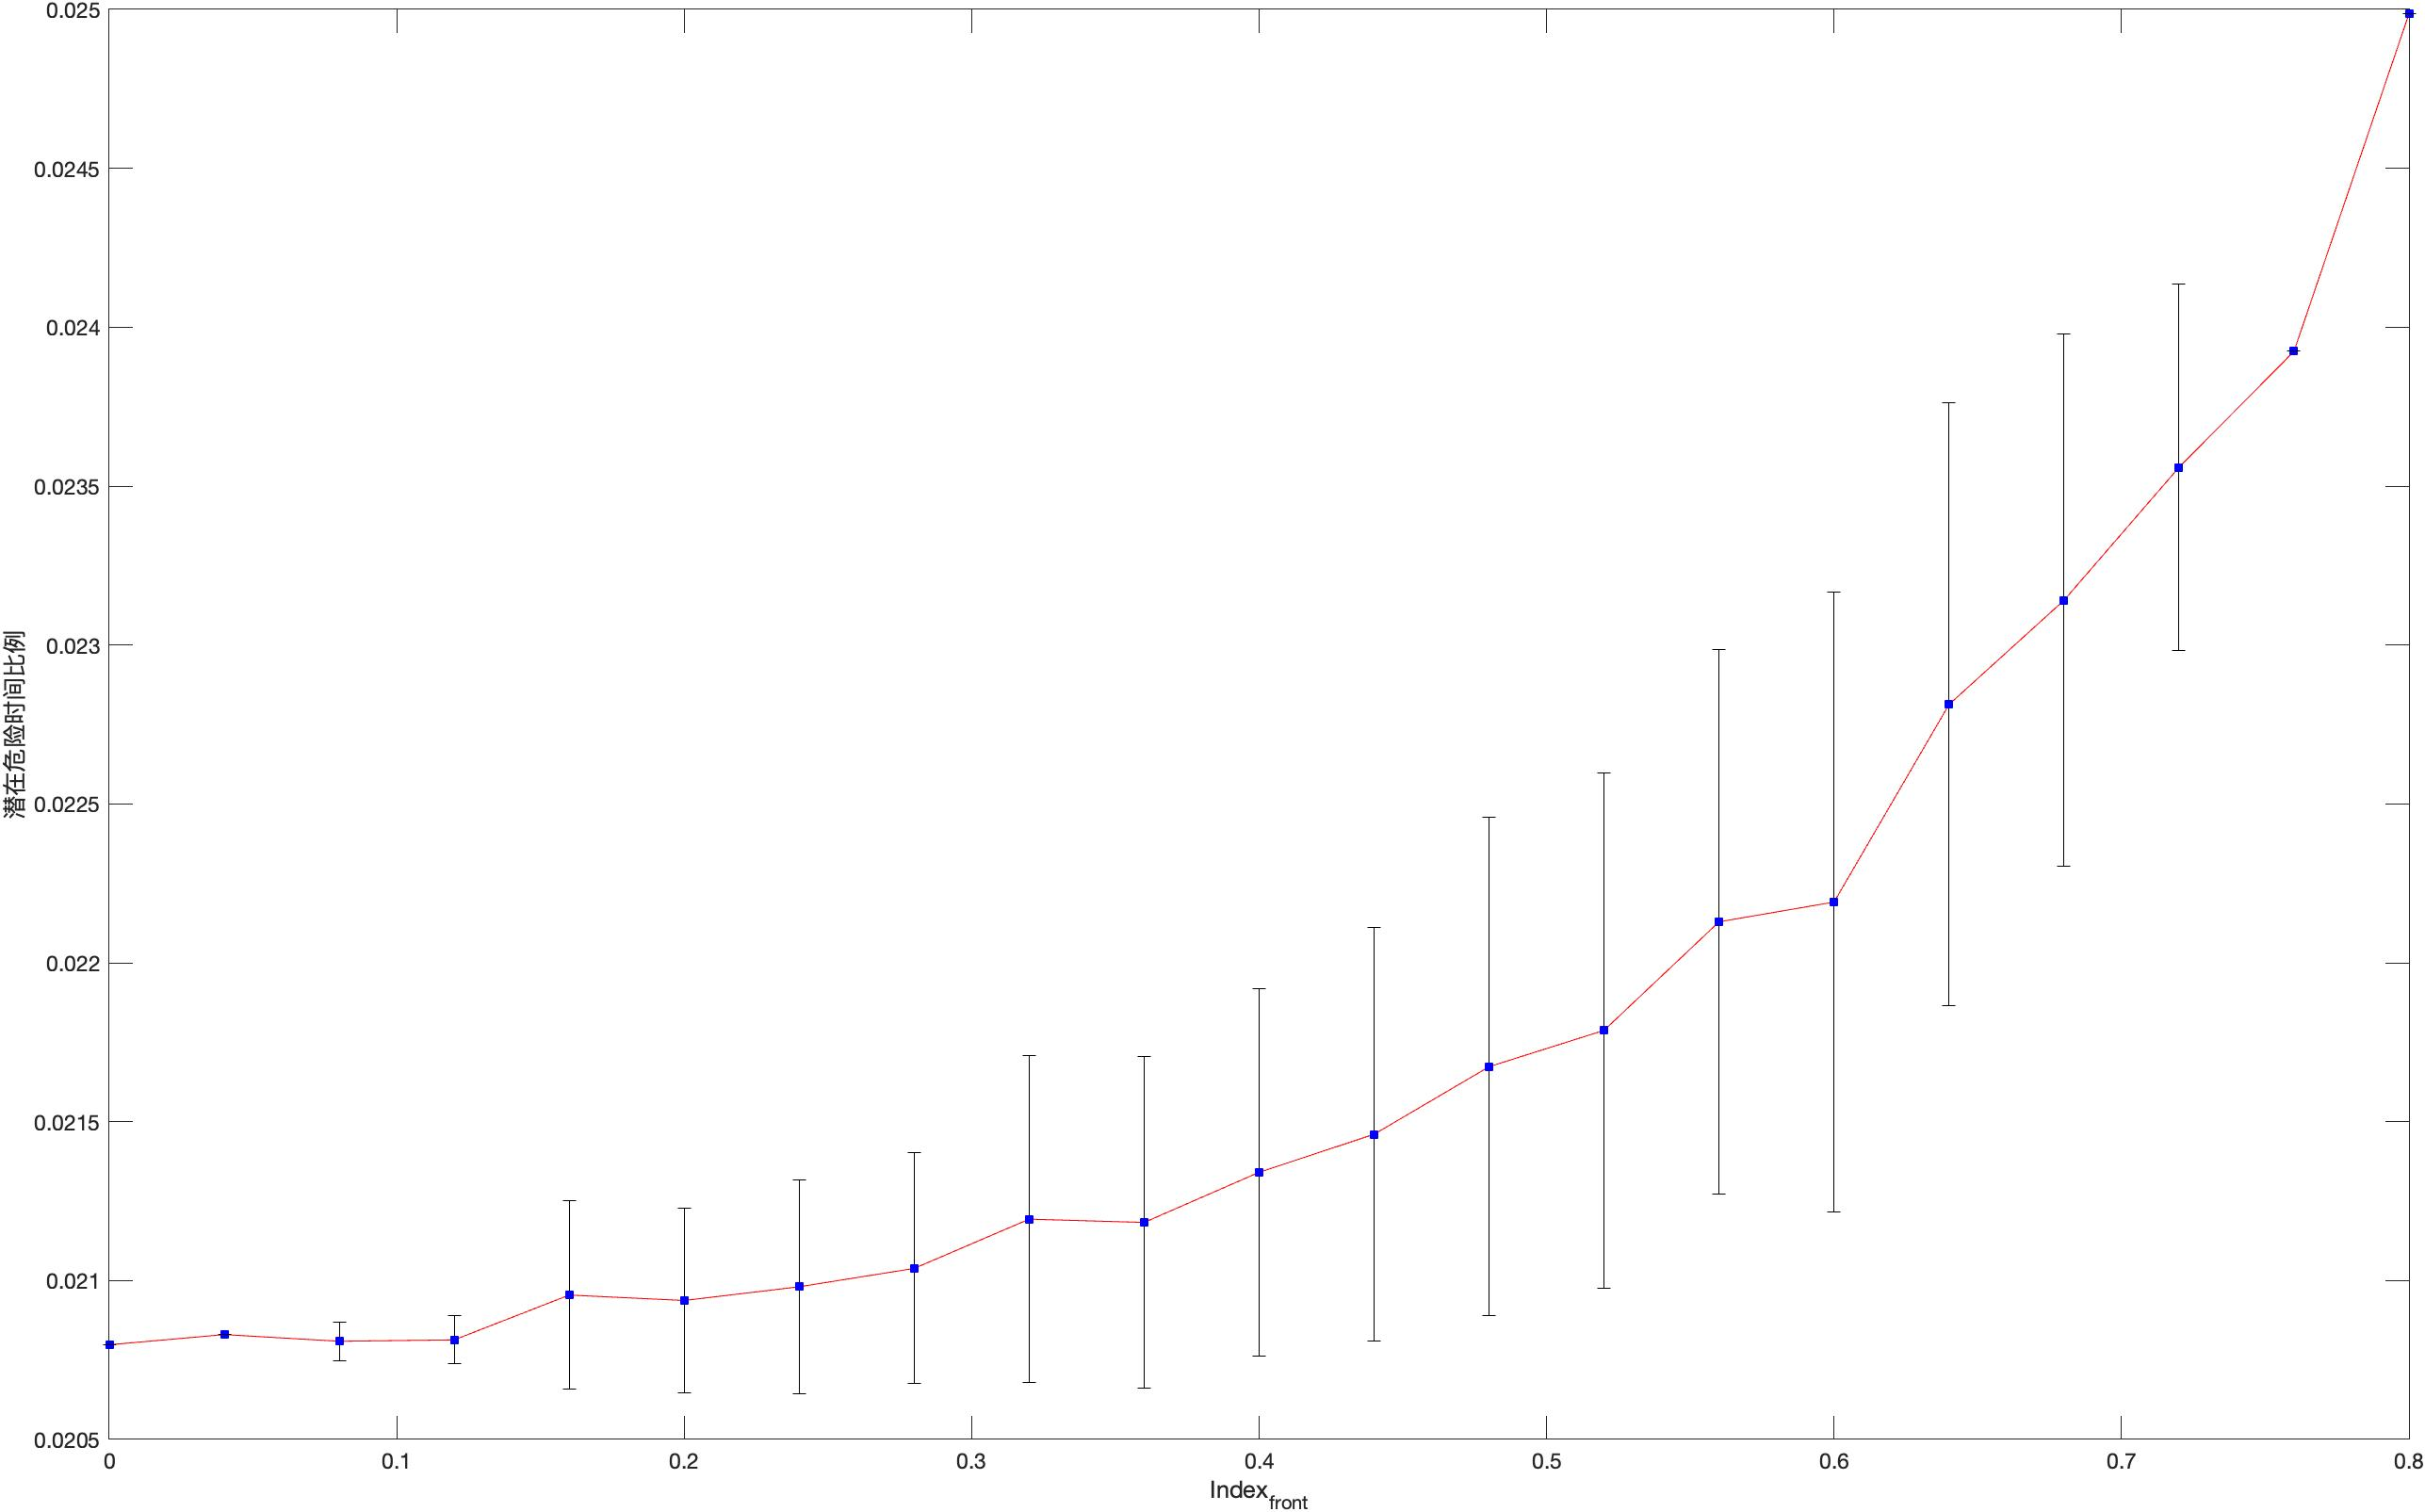
\includegraphics[width=1\linewidth]{chap04-front-PDT.jpg}
    \caption*{Error bar代表标准差}
    \caption{队首聚集度与潜在危险时间比例的关系}
    \label{fig:chap04-9}
\end{figure} 

可以发现二者呈正相关,其Pearson相关系数达到了0.6929。从此图可以看出。队首聚集度越大,自动驾驶车辆整体越远离头车,车队的潜在危险时间比例越大,车队整体越不安全,这与碰撞样本的碰撞风险演化机理是一致的,均呈现出队首聚集度越大,车队整体碰撞风险越大的规律。

图\ref{fig:chap04-9}所示的规律可以解释为:相比于自动驾驶车辆,人工驾驶车辆衰减扰动的能力更强,所以当自动驾驶车辆整体更靠近头车,扰动首先由自动驾驶车辆传递,并不断衰减,当传递到人工驾驶车辆时,扰动的幅度已减小了很多,再通过人工驾驶车辆传递,也不会造成太大的潜在危险。

为了对以上猜想进行验证,我们考虑一个给定排列的车队
\begin{equation}
    \leftarrow \{\mathrm{AV, AV, AV, AV, AV, HV, HV, HV, HV, HV}\} \notag
\end{equation}
其中AV代表人工驾驶车队,HV代表自动驾驶车队。仍给定初始均衡速度为$20m/s$观察每辆车的最大扰动,得到\ref{fig:chap04-10}所示结果。 \\\\

\begin{figure}
    \centering
    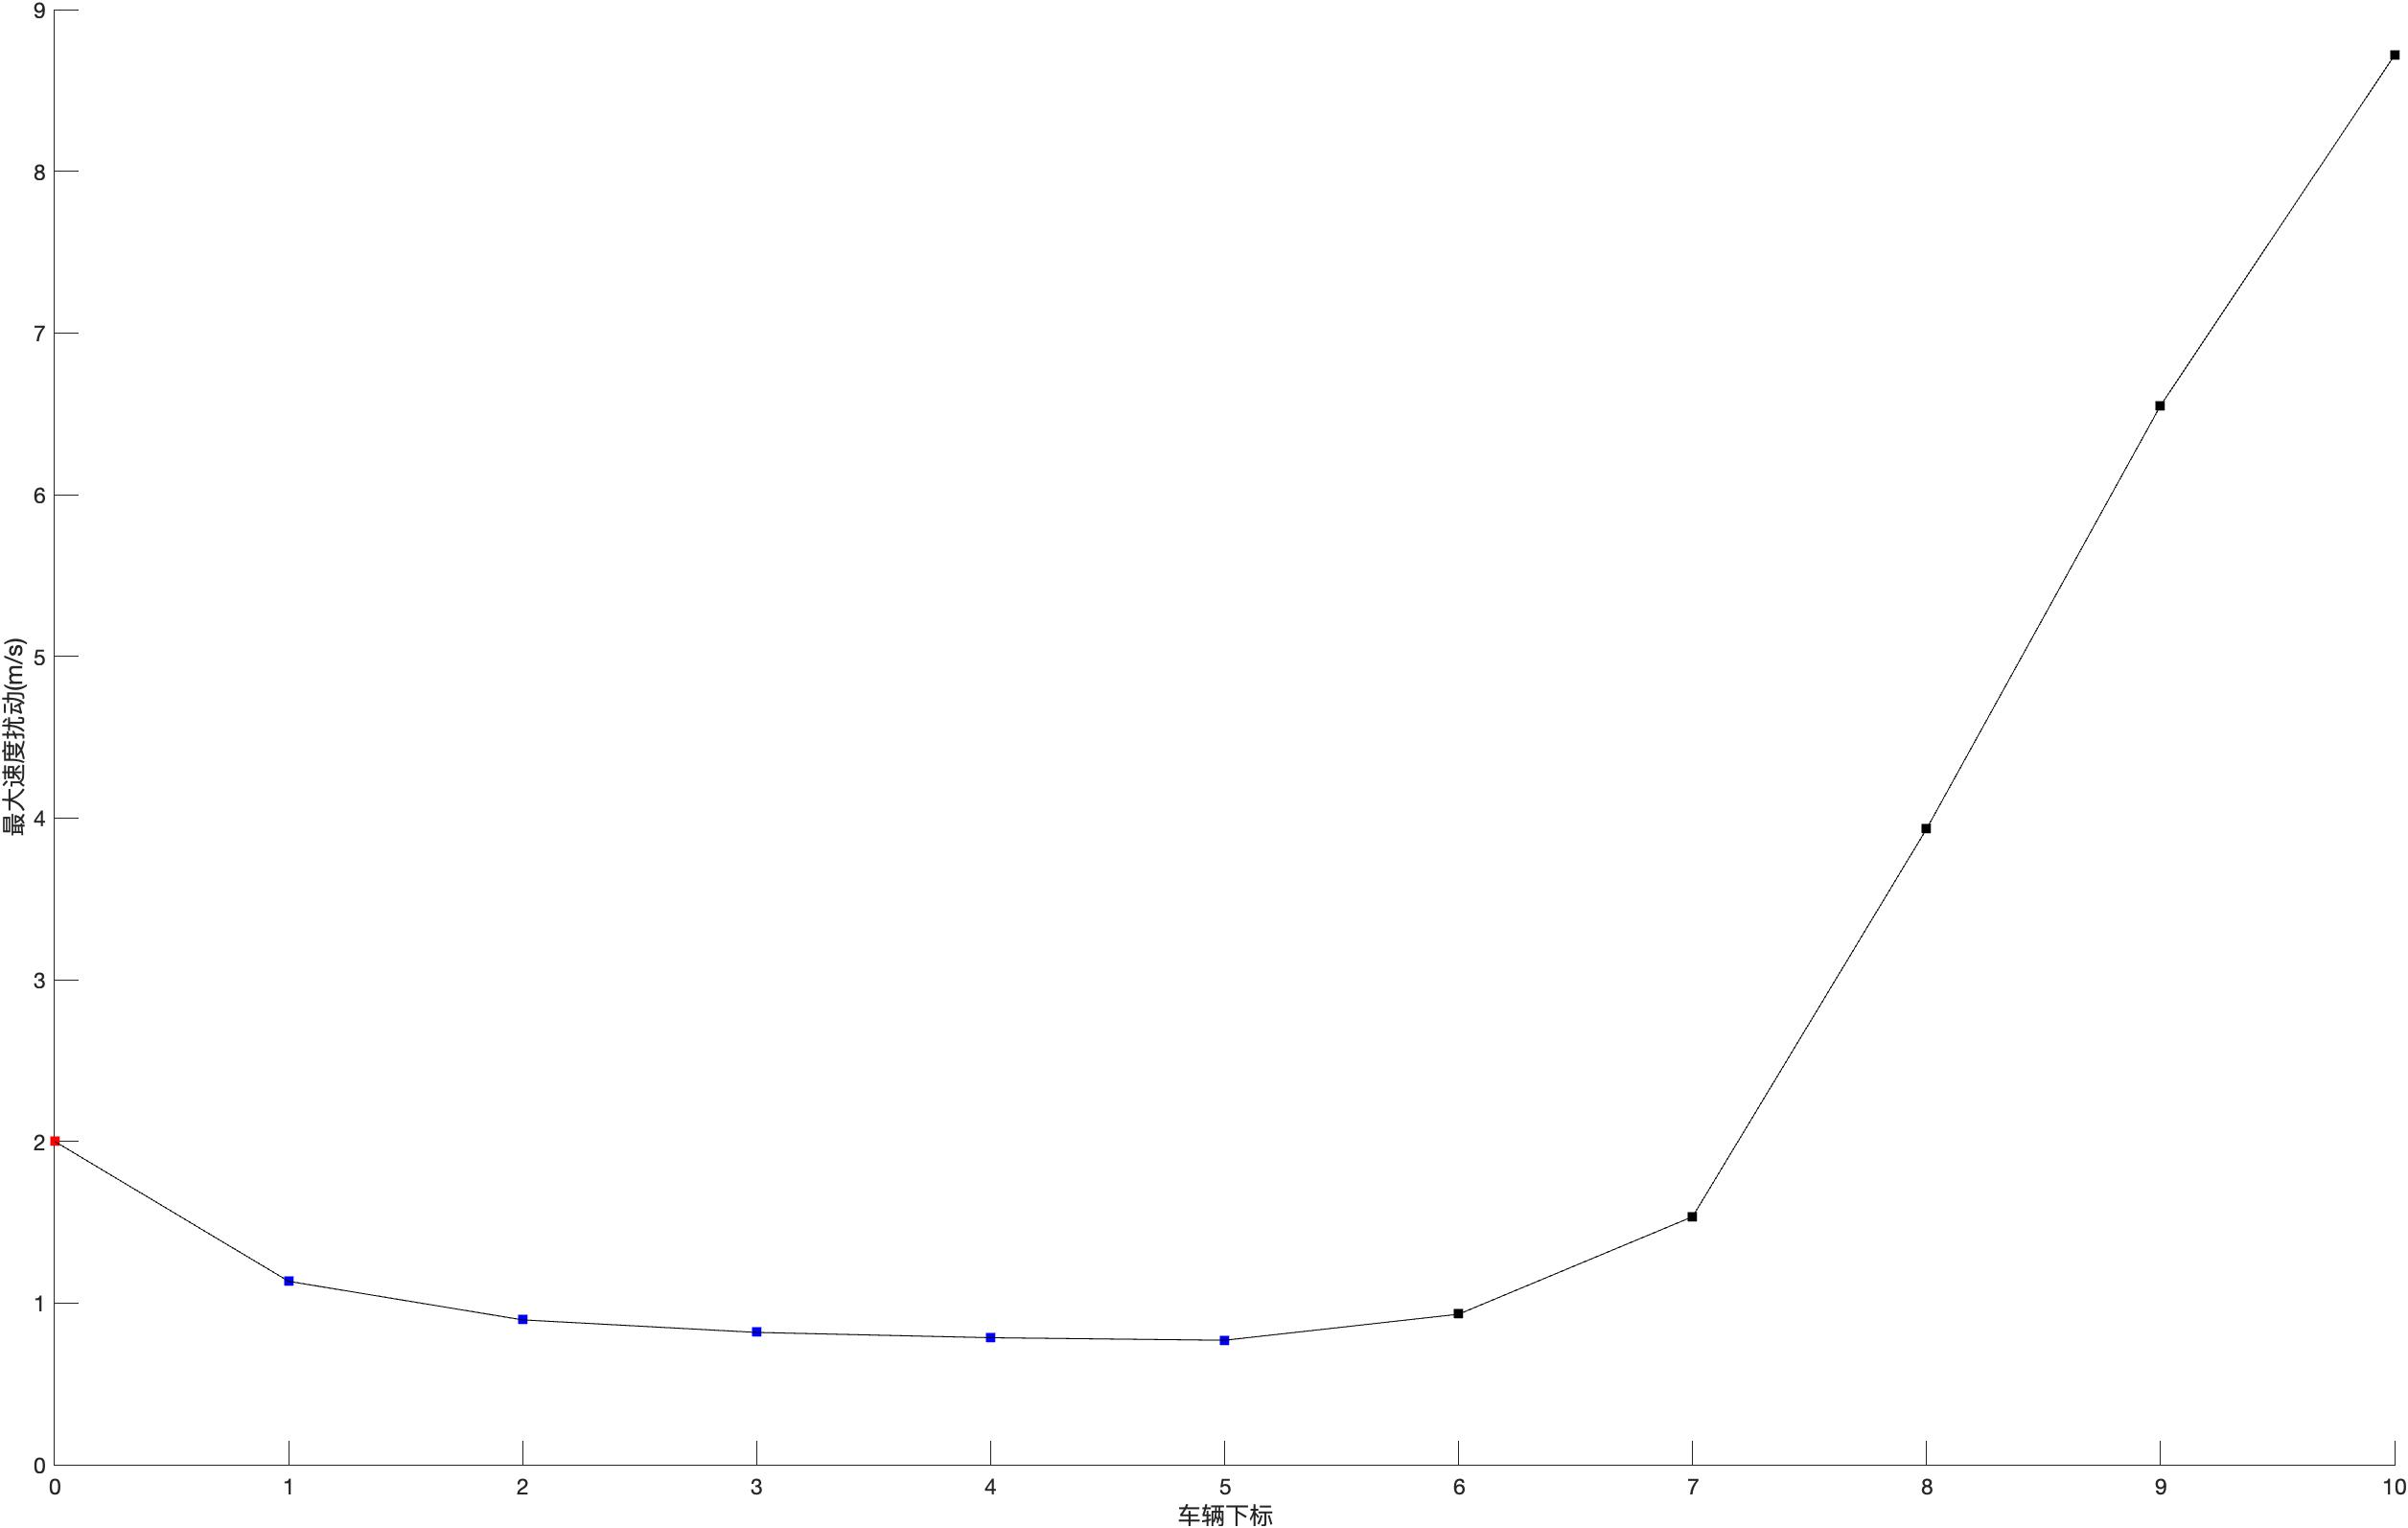
\includegraphics[width=1\linewidth]{chap04-index-delta.jpg}
    \caption*{红色样本点代表头车,蓝色样本点代表自动驾驶车辆,黑色样本点代表人工驾驶车辆}
    \caption{车队中各车最大扰动情况}
    \label{fig:chap04-10}
\end{figure} 

可以观察到对于自动驾驶车辆,即前5辆跟驰车辆,扰动大小呈下降的趋势,说明自动驾驶车辆有衰减扰动的效果,但对于人工驾驶车辆,即后5辆跟驰车辆,扰动被不断放大,这可能也是碰撞风险的主要来源。

\begin{figure}
    \centering
    \subcaptionbox{第3辆车跟驰车辆速度曲线\label{fig:chap04-7-1}}
      {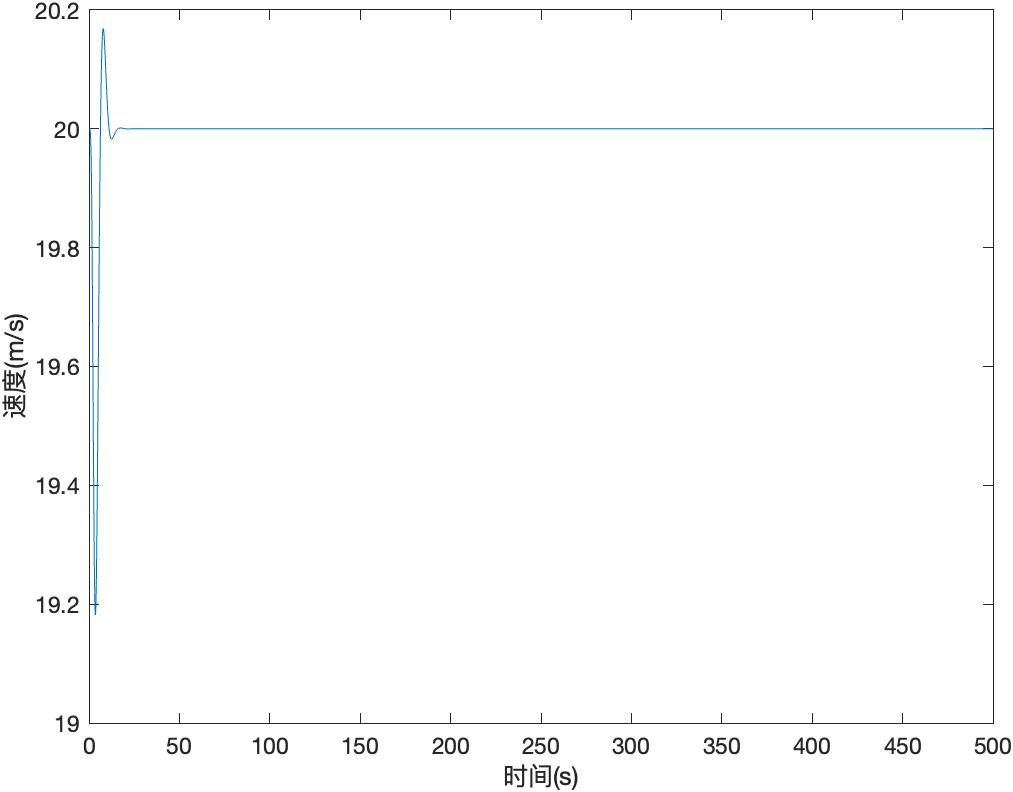
\includegraphics[width=0.49\linewidth]{chap04-3-AV.jpg}}
    \subcaptionbox{第8辆车跟驰车辆速度曲线 \label{fig:chap04-7-2}}
      {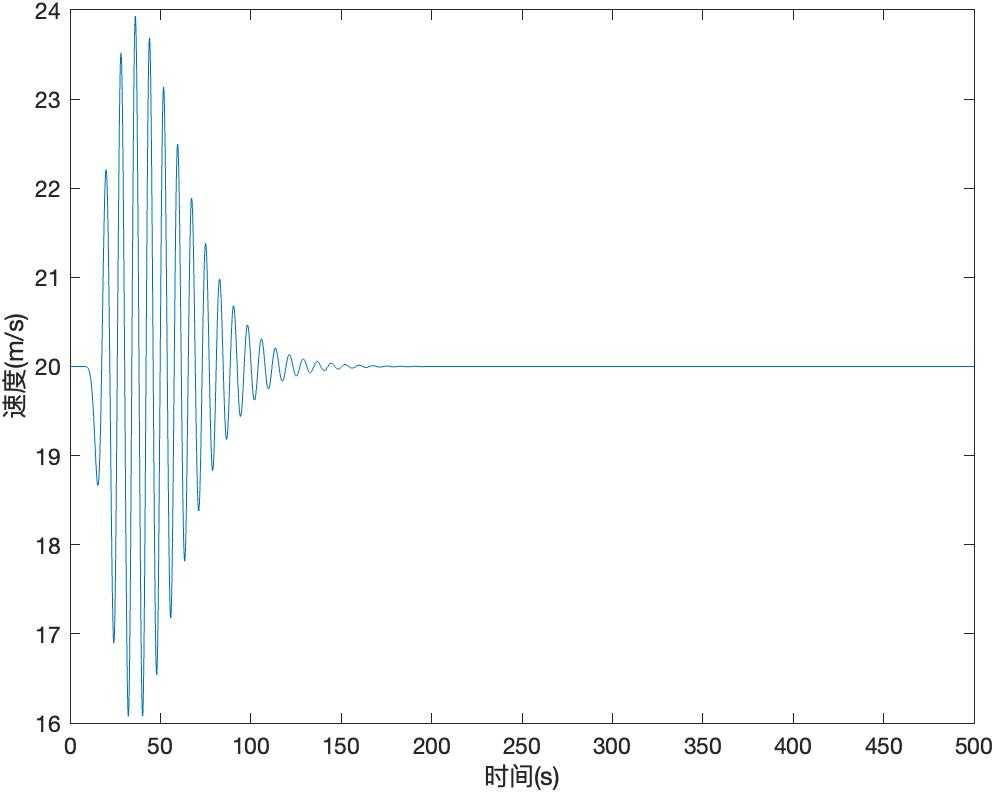
\includegraphics[width=0.49\linewidth]{chap04-car8-HV.jpg}}
      \caption{第3辆和第8辆跟驰车辆速度曲线}
    \label{fig:chap04-11}
  \end{figure}

图\ref{fig:chap04-11}显示了该实验中第3辆车跟驰车辆(自动驾驶车辆)和第8辆跟驰车辆(人工驾驶车辆)的速度曲线。可以发现第3辆车跟驰车辆速度扰动在不断衰减,而第8辆跟驰车辆的速度扰动先增大后衰减,这其实也和二者的稳定性有关,计算二者传递函数的无穷范数得到

\begin{equation}
    \begin{cases}
      \Vert G_{AV}(j\omega) \Vert_{\infty} < 1 \\
      \Vert G_{GV}(j\omega) \Vert_{\infty} > 1
    \end{cases}
    \label{eq:chap04-10}
\end{equation}

这说明虽然车队整体是队列不稳定的,但自动驾驶车辆是稳定的,其速度扰动会不断衰减;而人工驾驶车辆是不稳定的,其速度扰动会先增大,后减小。

即使是将5辆人工驾驶车辆和5辆自动驾驶车辆聚集在一起,5辆人工驾驶车辆跟驰5辆自动驾驶车辆的效果也是不同的,在该实验设定下,前车更为安全,因为在车队的前半段,自动驾驶车辆会先将扰动衰减再传递给人工驾驶车辆。

这样的规律也启示我们,对于真实场景,即使车辆有了不同的跟驰模型,也可以首先分析单车的稳定性,以单车的稳定性指导车队实现更低碰撞风险的排列。

图\ref{fig:chap04-12}所示是潜在危险时间比例与分散均匀度的关系。

\begin{figure}
    \centering
    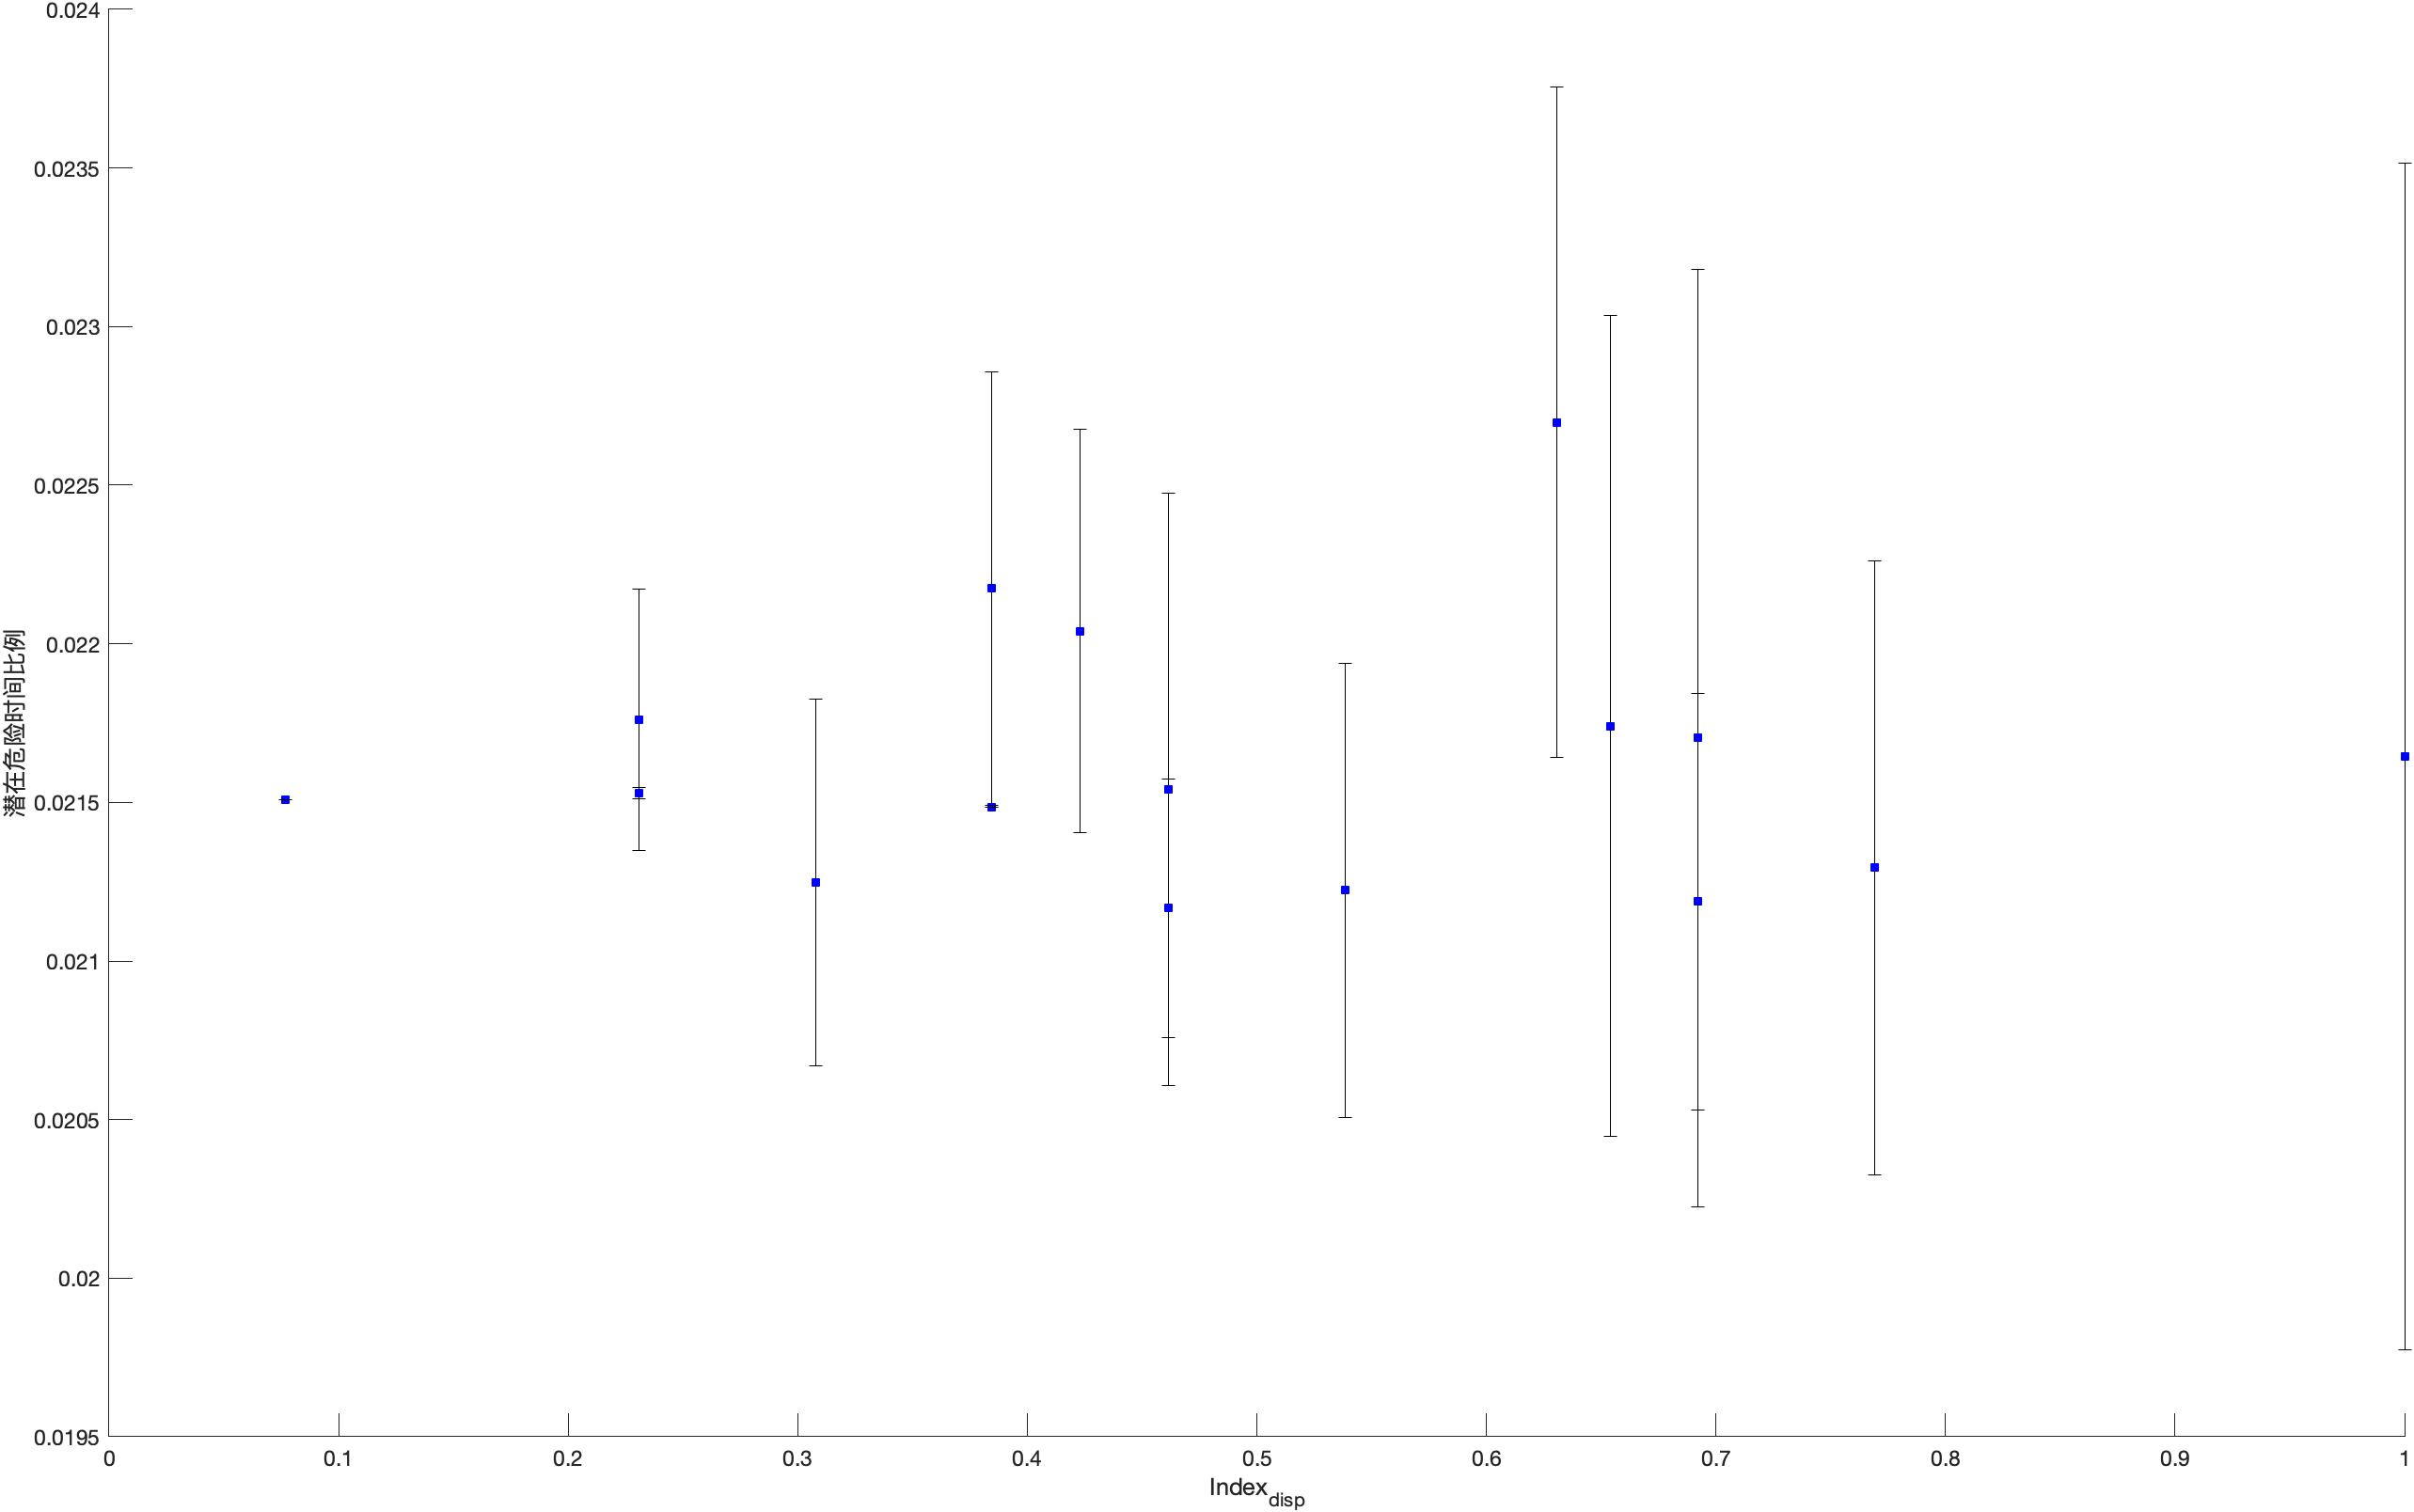
\includegraphics[width=1\linewidth]{chap04-disp-PDT.jpg}
    \caption{分散均匀度与潜在危险时间比例的关系}
    \label{fig:chap04-12}
\end{figure} 

可以发现分散均匀度与潜在危险时间比例并没有明显的关系,这与碰撞样本中二者的情况一致。

\section{本章小结}

在本章中,首先根据是否发生碰撞将实验样本分为了两大类,对于每一类分别选取了稳定性指标和碰撞风险指标。

混合车队的队列稳定性与碰撞风险之间的关系方面,研究发现,对于碰撞样本,车队的队列稳定性越好,碰撞越晚发生,且碰撞越靠近队尾;对于非碰撞样本,车队的队列稳定性越好,车队整体的潜在危险时间比例越低,即车队整体的碰撞风险更小。

混合车队的碰撞风险演化机理方面,首先选择了队首聚集度和分散均匀度这2个车队空间分布指标,研究发现,无论是对于碰撞样本还是对于非碰撞样本,碰撞风险的演化都与队首聚集度有关,而与分散均匀度无明显关系。

图\ref{fig:chap04-strcture}描述了本章的结构。

\begin{figure}
    \centering
    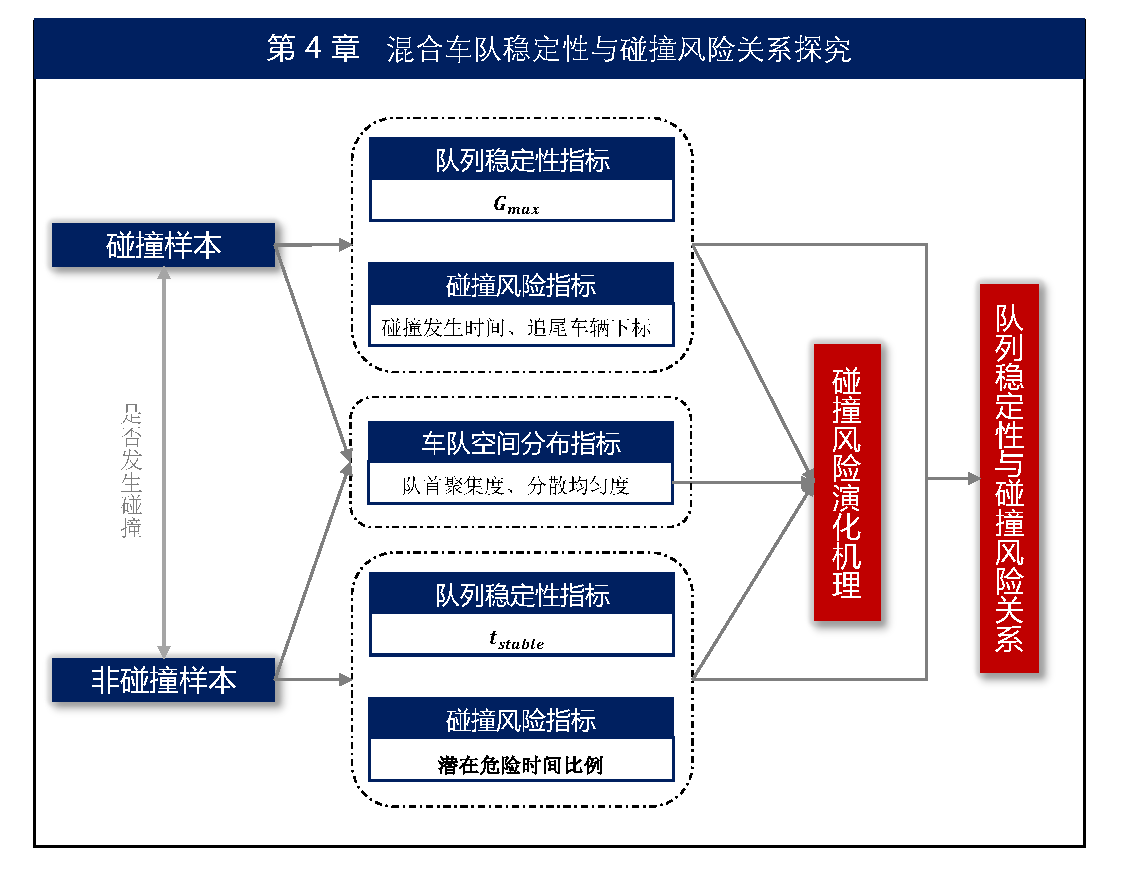
\includegraphics[width=1\linewidth]{chap04-structure.pdf}
    \caption{第4章结构}
    \label{fig:chap04-strcture}
\end{figure} 




% 其他部分
\backmatter

% 参考文献
\bibliography{ref/refs}  % 参考文献使用 BibTeX 编译
% \printbibliography       % 参考文献使用 BibLaTeX 编译

% 附录
% 本科生需要将附录放到声明之后,个人简历之前
\appendix
% % !TeX root = ../thuthesis-example.tex

\begin{survey}
\label{cha:survey}

\title{Title of the Survey}
\maketitle


\tableofcontents


本科生的外文资料调研阅读报告。


\section{Figures and Tables}

\subsection{Figures}

An example figure in appendix (Figure~\ref{fig:appendix-survey-figure}).

\begin{figure}
  \centering
  
\includegraphics[width=0.6\linewidth]{example-image-a.pdf}
  \caption{Example figure in appendix}
  \label{fig:appendix-survey-figure}
\end{figure}


\subsection{Tables}

An example table in appendix (Table~\ref{tab:appendix-survey-table}).

\begin{table}
  \centering
  \caption{Example table in appendix}
  \begin{tabular}{ll}
    \toprule
    File name       & Description                                         \\
    \midrule
    thuthesis.dtx   & The source file including documentaion and comments \\
    thuthesis.cls   & The template file                                   \\
    thuthesis-*.bst & BibTeX styles                                       \\
    thuthesis-*.bbx & BibLaTeX styles for bibliographies                  \\
    thuthesis-*.cbx & BibLaTeX styles for citations                       \\
    \bottomrule
  \end{tabular}
  \label{tab:appendix-survey-table}
\end{table}


\section{Equations}

An example equation in appendix (Equation~\eqref{eq:appendix-survey-equation}).
\begin{equation}
  \frac{1}{2 \uppi \symup{i}} \int_\gamma f = \sum_{k=1}^m n(\gamma; a_k) \mathscr{R}(f; a_k)
  \label{eq:appendix-survey-equation}
\end{equation}


\section{Citations}

Example citations in appendix.
\cite{abrahams99tex}
\cite{salomon1995advanced}
\cite{abrahams99tex,salomon1995advanced}


\bibliographystyle{unsrtnat}
\bibliography{ref/appendix}

\end{survey}
       % 本科生:外文资料的调研阅读报告
% % !TeX root = ../thuthesis-example.tex

\begin{translation}
\label{cha:translation}

\title{车队的队列稳定性:定义和分析方法}
\maketitle

% \tableofcontents

  \vspace{1em}
  \textbf{摘要:}由互相关联的自动驾驶车辆 (connected and automated vehicles, CAVs) 组成的车队预计将对道路交通产生变革性影响,例如提高高速公路安全性、提高交通效率和减少燃料消耗。控制车队时的一项关键任务是实现队列稳定性(String Stability),
  为此提出了许多模型和算法。但是,尽管这些年来针对队列稳定性提出了许多不同的定义和分析方法,但是没有进行详尽的比较。 为了填补这些空白,本文旨在阐明这些模糊的定义与各种分析方法之间的关系,为今后的研究提供一个坚实
  的基础。本文总结和讨论了一系列等价的定义和算法,也讨论了不同分析方法和定义的优、缺点。 所有这些讨论为在实际使用中选择车队的分析方法提供了见解。

\section{引言}

  作为一种提高交通效率的有效方式,车队控制引起了广泛的兴趣。(Guanetti, Kim, and Borrelli, 2018; Horowitz and Varaiya, 2000; Ioannou and Chien,1993; Li, Zheng, Li, and Wang, 2015; Sheikholeslam and Desoer, 1990; Shladover, 1995)
  在一个车队中,由两辆及以上车辆组成的车队按照预先设置的巡航速度和车间距行驶。与人工驾驶相比,自动驾驶车队有着车与车之间的距离更小的优点(即队形更加紧密),被认为是一个很有希望的降低交通阻塞、空气阻力和燃油损耗的方法。
  (Al Alam, Gattami, and Johansson, 2010; Chien and Ioannou, 1992; Liand Chen, 2017)
  
  车队的紧密编队控制有一个特殊的困难,称为“队列不稳定性”,即系统中的扰动沿着车队不断放大,如图~\ref{fig:appendix-translation-figure1}(b)所示(参见Peppard(1974))。 
  正如观察 (Treiterer and Myers, 1974) 和实验 (Sugiyama et al., 2008) 所证明的那样,紧密编队车队的队列不稳定性会导致在环形线路和高速公路上出现没有瓶颈的堵塞(例如,走走停停),这严重损害了车队控制的好处。

\begin{figure}
  \centering
  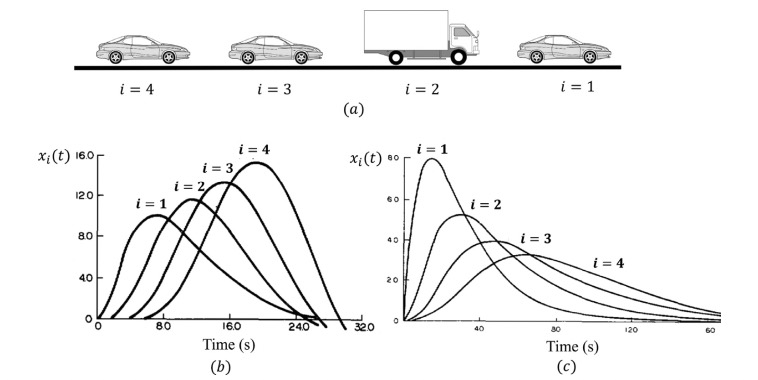
\includegraphics[width=1\linewidth]{appendix-A-1.jpg}
  \caption{车队系统图示(a)和队列稳定性的直观描述(b-c)(Peppard, 1974),其中$x_i(t)$表示车辆$i$在时间$t$的状态波动(例如位置误差)。}
  \label{fig:appendix-translation-figure1}
\end{figure}
   
  为了解决这个问题,队列稳定性的性质已经被广泛研究并应用于车队控制。直观地说,如果一个车队具有以下特性,则称它是队列稳定的,即扰动不会沿着车队被不断放大(Peppard,1974),
  如图~\ref{fig:appendix-translation-figure1}(c)所示。研究队列稳定性的基本过程可分为三个步骤:(1)数学上定义队列稳定性的性质;(2)根据分析方法推导出充分条件;(3) 设计控制器以满足充分条件

\subsection{研究动机}

  大量文献提出了很多种不同的的定义和分析方法。在许多研究中,虽然仿真结果显示出与图~\ref{fig:appendix-translation-figure1}(c)相似的性质,但队列稳定性的性质存在令人困惑的差异。
  许多不同的定义是基于不同的域(例如频域和时域)和范数(例如$\mathcal{L_2}$、$\mathcal{L_p}$和$\mathcal{L_\infty}$)、强度(例如弱和强)。模棱两可的定义阻碍了不同研究之间的比较。
  需要对它们之间的关系进行严格的分析以帮助进一步研究的进行。此外,学者已经提出了许多分析方法并衍生了许多性质,它们的关系、利弊以及可以解决什么问题尚未得到太多讨论。
  更好地理解这些方法和性质是进一步研究困难问题的基础。

\subsection{研究范围和目的}

本文重点介绍队列稳定性的定义和推导队列稳定性质的分析方法。为了更好地解释相关概念,我们将简要介绍一些车队控制的研究工作。然而,为了简明扼要,本文将不讨论车队控制领域的其他问题。
(Li et al., 2015; Li, Zheng et al., 2017)。

本文的目的是:(1)阐明队列稳定性模糊定义之间的关系,提出统一的定义; (2)讨论各种分析方法的关系、利弊、可以解决什么问题,并针对存在的棘手问题提出方法建议;(3)深入研究各性质之间的关系,
这为解决队列不稳定的问题提供了思路。

\subsection{主要贡献}

  本工作的主要贡献为:

  第一,严格分析了模糊不清的定义之间的关系。对常用的定义进行了介绍和比较。总结了队列稳定性的三个基本属性,即收敛性、有界性和可扩展性。类似于控制理论中稳定性定义,
  本文提出了三种类型的队列稳定性定义作为不同定义之间的桥梁,即李雅普诺夫稳定性、输入-输出稳定性和输入-状态队列稳定性。定理1详细阐述了对这些队列稳定性定义的严格分析。
  受该定理的启发,建议将所提出的定义,即输入-状态队列稳定性 (ISSS)用于未来的研究。,并且给出了推荐ISSS的理由。本文扩展并深化了对该领域先前主要对定义的讨论。
  (Ploeg, Van De Wouw, and Nijmeijer, 2014; Stüdli, Seron, and Middleton, 2017)

  第二,本文对各种分析方法进行了比较,并对通过使用这些分析方法推导得到的性质进行了严格的分析。这些方法可以分为三类:时间域分析方法、$z$域分析方法和$s$域分析方法。
  带分析的问题可分为时间维度和空间维度。本文分别从两个维度讨论了这些分析方法的优缺点,在此基础上我们推荐了针对现有困难问题的方法。此外,在定理2中对推导得到的性质进行了严格分析,
  从中展现了这些性质以及常用研究队列系统的推荐定义(即ISSS)之间的关系。 并将解决队列不稳定的常用解决方法与“弱耦合性质”进行了比较。

\section{预备知识}
  记实数域为$\mathbb{R}$,自然数集$\mathbb{N}={1, 2, \dots}$,对于向量$\chi \in \mathbb{R}^n$,其$p$范数为
  \begin{equation}
    \Vert\chi\Vert_p = \left( \sum_{i=1}^n{|\chi_i|^p} \right) ^{1/p}, p \in [1, \infty)
    \label{eq:appendix-equation-1}
  \end{equation}
  \begin{equation}
    \Vert\chi\Vert_\infty = \max_{i} |\chi_i|.
    \label{eq:appendix-equation-2}
  \end{equation}
  对于一个勒贝格可测的信号$\chi(t):I \rightarrow \mathbb{R}^n$,其$\mathcal{L}_p$范数$\Vert\chi\Vert^I_{\mathcal{L}_p}$定义为
  \begin{equation}
    \Vert\chi\Vert^I_{\mathcal{L}_p} = \left( \int_I{\Vert\chi\Vert_p^p dt} \right) ^{1/p} < \infty, p \in [1, \infty)
    \label{eq:appendix-equation-3}
  \end{equation}
  \begin{equation}
    \Vert\chi\Vert^I_{\mathcal{L}_\infty} = \sup_{t \in I} \Vert\chi\Vert_\infty,
    \label{eq:appendix-equation-4}
  \end{equation}
  当$I=[0, \infty)]$时,$\Vert\chi\Vert^{[0, \infty)]}_{\mathcal{L}_\infty}$简记为$\Vert\chi\Vert_{\mathcal{L}_\infty}$。给定一个系统的传递函数$G(j\omega)$,系统的$\mathcal{H}_\infty$范数定义为
  \begin{equation}
    \Vert G \Vert_{\mathcal{H}_\infty} = \sup_{\omega}|G(j\omega)|, {\rm (SISO)}
    \label{eq:appendix-equation-5}
  \end{equation}
  \begin{equation}
    \Vert G \Vert_{\mathcal{H}_\infty} = \sup_{\omega}\bar{\sigma} \left( G(j\omega) \right), {\rm (MIMO)}
    \label{eq:appendix-equation-6}
  \end{equation}
  SISO代表单输入单输出系统,MIMO代表多输入多输出系统。$\bar{\sigma} \left( G(j\omega) \right)$是矩阵$G(j\omega)$的最大奇异值(参见Zhou, Doyle, Glover et al., 1996)。
  对于连续函数$\alpha:[0, a) \rightarrow [0, \infty), a \in \mathbb{R}^+$,如果在其定义域上是严格单调递增的,并且$\alpha(0) = 0$,那么我们称这个函数是$\mathcal{K}$类函数。
  对于连续函数$\beta:[0, a) \times [0, \infty) \rightarrow [0, \infty)$,如果对于每一个固定的$s$,函数$\beta(\cdot, s)$是$\mathcal{}$类函数,并且对于每一个固定的$r$,函数$\beta(r, \cdot)$
  在其定义域上是单调递减的,且满足当$s \rightarrow 0$时,$\beta (r, s) \rightarrow 0$,那么我们称这个函数是$\mathcal{KL}$类函数。如果$\Vert\chi\Vert_{\mathcal{L}_\infty} < \infty$,我们
  称$\chi \in \mathcal{L}_\infty$。

  通常,我们考虑一个车队
  \begin{align}
    \dot{\chi} &= f(\chi, \omega), \\
    \label{eq:appendix-equation-7}
    y &= g(\chi)
  \end{align}

  这里,函数$f(\chi, \omega): \mathbb{R}^{mn} \times \mathbb{R}^m \rightarrow \mathbb{R}^{mn}$是连续可导且全局Lipschitz的,
  函数$g(\chi): \mathbb{R}^{mn} \rightarrow \mathbb{R}^{m}$是连续可导且全局Lipschitz的。$\chi \in \mathbb{R}^{mn}$代表系统状态向量,
  $\omega \in \mathbb{R}^m$代表扰动。我们假设原点$\chi = 0$是非受迫系统$\dot{\chi} = f(\chi, 0)$的一个稳定平衡点。对于车队,$m \in \mathbb{N}$
  代表了车队长度,$n \in \mathbb{N}$代表子系统的状态阶数,表\ref{tab:appendix-translation-table1}列出了这些符号的含义。

  \begin{table}
    \centering
    \caption{所用变量的符号}
    \begin{tabular}{ll}
      \toprule
      变量          & 符号                        \\
      \midrule
      $S_m$           & $S_m = \{0\} \cup \{i \in \mathbb{N} | 1 \leqslant i \leqslant m-1 \}.$ \\
      $S_{e,m}$       & $S_m = \{i \in \mathbb{N} | 1 \leqslant i \leqslant m-1 \}.$                     \\
      $\chi_i(t)$     & $\chi_i(t) \in \mathbb{R}^n$代表第$i$个子系统的状态   \\
      $\omega_i(t)$   & $\omega_i(t) \in \mathbb{R}$代表第$i$个子系统受到的扰动 \\
      $y_i(t)$        & $y_i(t) \in \mathbb{R}$代表第$i$个子系统的输出        \\
      $\chi_i(t)$     & $\chi_i(t) \in \mathbb{R}^{mn}$代表系统的状态        \\
      $\omega(t)$     & $\omega(t) \in \mathbb{R}^m$代表系统受到的扰动        \\
      $y(t)$          & $y(t) \in \mathbb{R}^m$代表系统的输出        \\
      $\Chi_i(s), Y_i(s), U_i(s)$   & $\chi_i(t), y_i(t), u_i(t)$的拉普拉斯变换        \\
      $\Chi(s), Y(s), U(s)$         & $\chi(t), y(t), u(t)$的拉普拉斯变换        \\
      $\mathcal{\Chi}(z), \mathcal{Y}(z), \mathcal{U}(z)$   & $\chi(t), y(t), u(t)$的$z$变换        \\
      \bottomrule
    \end{tabular}
    \label{tab:appendix-translation-table1}
  \end{table}


\section{车队控制}

本节简要介绍了车队的控制问题,该问题引发了对队列稳定性的研究。车队的控制问题最初由Levine和Athans于1966年提出,研究如何设计一个控制器来实现队列系统的控制。
这包括队列系统描述、控制目标和控制器设计方法。并且介绍了本文的两个重点的背景,即队列稳定性的定义和分析方法。

\subsection{队列系统描述}

车队系统的描述确定了队列稳定问题的研究场景。本文采用了由四个部分组成的框架(Li et al., 2015),即节点动力学、信息流拓扑结构、分布式控制和构成几何。
此外,还强调了系统的通信质量和收到的干扰。一个特定的车队系统可以通过这六个部分来唯一确定,本小节中用到的缩写在表\ref{tab:appendix-translation-tableA1}中列出。

\subsubsection{节点动力学}

节点动力学(node dynamics, ND)表示车辆在纵向的动力学。根据建模,车辆动力学模型可分为非线性(Dunbar and Caveney, 2012; Rajamani, 2011),
二阶模型(Naus, Vugts, Ploeg, van de Molengraft, and Steinbuch, 2010; Yanakiev and Kanellakopoulos, 1996),
三阶模型(Godbole and Lygeros, 1994; Liang and Peng, 1999; Warnick and Rodriguez, 2000),和一般线性模型(Liang and Peng, 2000; Seiler, Pant, and Hedrick, 2004)。

\subsubsection{信息流拓扑结构}

信息流拓扑结构(information flow topology, IFT)描述了车辆如何与其他车辆交换信息。图\ref{fig:appendix-translation-figure2}所示为常用的拓扑结构,包括前继跟随拓扑(PF)(Naus et al., 2010)、
前继领导跟随拓扑(PLF)(Sheikholeslam and Desoer, 1990; Swaroop and Hedrick, 1999)、
双向拓扑(BD)(Eyre, Yanakiev, and Kanellakopoulos, 1997; Ghasemi, Kazemi, and Azadi, 2013; Knorn, Donaire, Agüero, and Middleton, 2014; Yanakiev and Kanellakopoulos, 1996),
双向领导拓扑(BDL)(Zheng, Li, Wang, Cao, and Li, 2016),
双前继跟随拓扑(TPF)(Swaroop and Hedrick, 1999),
以及双前继领导跟随拓扑(TPLF)(Li et al., 2015)。
也可以应用更一般的信息流拓扑结构,例如,$r$前继跟随拓扑($r$PF)和$r$前继领导跟随拓扑($r$PLF),其中$r$表示有之交流的前继数量。

\begin{figure}
  \centering
  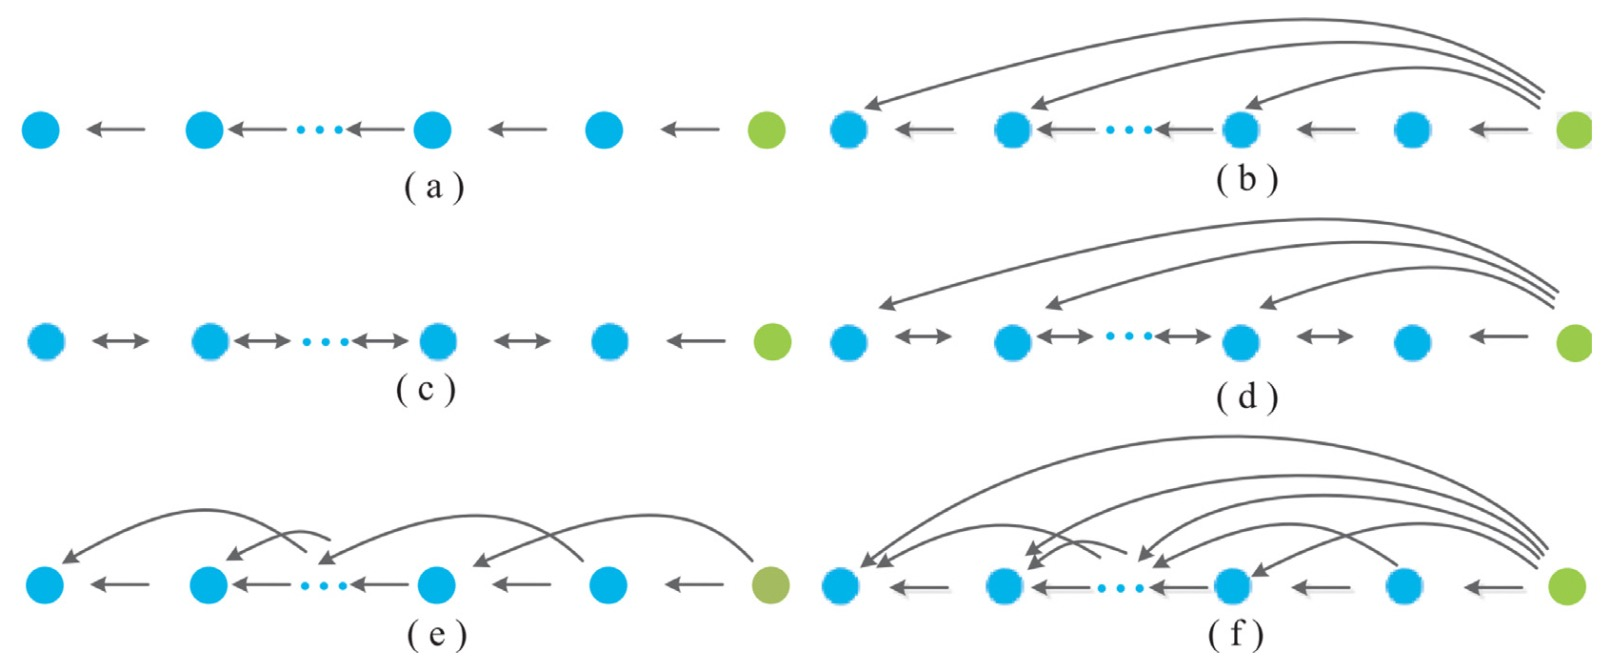
\includegraphics[width=1\linewidth]{appendix-A-2.jpg}
  \caption{车队的的典型信息流拓扑结构,其中绿色圆圈表示头车。(a)PF;(b)PLF;(c)BD;(d)BDL;(e)TPF;(f)TPLF(Li et al., 2015)。}
  \label{fig:appendix-translation-figure2}
\end{figure}

\subsubsection{分布式控制器}

分布式控制器(distributed controller, DC)描述了用于实现控制目标的对车队系统的控制器,例如,线性控制器(Nauset al.,2010;Sheikholeslam and Desoer,1993)、
最优控制器(Chu,1974b;Jin and Orosz,2017;Liang and Peng,1999)、$H_\infty$控制器(Ploeg, Shukla, van de Wouw, and Nijmeijer,2014)、
模型预测控制(MPC)(Dolk, Ploeg, and Heemels, 2017; Dunbar and Caveney, 2012),以及滑模控制(SMC)(Fernandes and Nunes,2012)。

\subsubsection{构成几何}

车队的构成几何(formation geometry, FG)表示车队所期望的车辆间距离,在许多研究中也被称为间距策略。现在存在三种主要政策,
即恒定距离(constant distance, CD)政策(Liu, Goldsmith, Mahal., and Hedrick, 2001; Sheikholeslam and Desoer, 1993)、
恒定时间间隔( constant time headway, CTH)政策(Chien and Ioannou, 1992; Zhou and Peng, 2005),
以及非线性距离(nonliear distance, NLD)政策(Orosz, 2016; Santhanakrishnan abd Rajamani, 2003)。

\subsubsection{通信质量}

通信质量(communication quality, CQ)描述了由其引起的问题,即通信时间延迟(di Bernardo, Salvi, and Santini, 2015; Liu et al., 2001; Oncu, Van de Wouw, 
Heemels, and Nijmeijer, 2012; Qin, Gomez, and Orosz, 2017; Xiao, Darbha, and Gao, 2008; Xiao, Gao, and Wang, 2009)
和丢包(Moreau, 2005; Ploeg, Semsar-Kazerooni, Lijster, van de Wouw, and Nijmeijer, 2015; Teo, Stipanovic, and Tomlin, 2002; 2003)。

\subsubsection{扰动}

扰动是造成车队系统产生偏差的原因,常用的扰动类型包括:
\begin{itemize}
  \item 第一类:头车的初始条件扰动;
  \item 第二类:所有车辆的初始条件扰动;
  \item 第三类:头车受到的零初始条件外部扰动;
  \item 第四类:所有车辆受到的零初始条件外部扰动。
\end{itemize}


最后,介绍两个车队系统的重要术语,即同质性和无限性。如果所有车辆都具有相同的动力学特性,则称该车队具有同质性(Chu,1974a);否则称其具有异质性(Naus等,2010)。
此外,如果车队有无限辆车辆组成,则称其为无限的(Swaroop and Hedrick, 1996);否则称为有限的(Jin and Orosz, 2014)。
理论分析使得研究人员可以通常研究无限车队,以研究由大量但有限辆车组成的车队的本质(Curtain, Iftime, and Zwart, 2010; Jovanovic and Bamieh, 2005)和车队的可扩展性。

\subsection{控制目标}

控制自动驾驶车辆车队的目的是确保同一组的所有车辆以一致的速度移动,同时相邻车辆之间保持理想距离,从而提高交通容量,改善交通安全性,并减少燃料消耗(Horowitz and Varaiya, 2000)。
车队系统的稳定性特性是上述所有控制目标的基础。研究人员已经提出了两种类型的稳定性,个体稳定性和队列稳定性。

个体稳定性描述了车辆向给定轨迹收敛的情况(Dolk et al., 2017; Dunbar and Caveney, 2012; Ghasemi et al.,2013; Guo, Ding, and Han, 2014; Ploeg,Shukla et al., 2014; Swaroop and Hedrick, 1999; Zheng, Li, Wang et al., 2016),
收敛速度由稳定系数描述(Barooah, Mehta, and Hespanha, 2009; Hao and Barooah, 2012; Hao, Barooah, and Mehta, 2011; Zheng, Li, Li, and Wang, 2016)。
然而,随着长度的增加,一个每个个体都稳定的车队仍然可能将一个小的扰动放大并造成交通拥堵(例如走走停停)(Hedrick, Tomizuka, and Varaiya, 1994; Naus et al., 2010。 Shaw and Hedrick, 2007b; Sugiyama et al., 2008)。

为了解决这个问题,研究人员提出了队列稳定性并对其做了大量研究。直观地说,如果扰动在沿车队向下游传播时不被放大,那么就可以说车队是队列稳定的(Peppard, 1974)。
为了从数学上定义这一特性,在过去的几十年里,针对不同的车队系统提出了各种正式的队列稳定定义,例如(Jin and Orosz, 2014; Khatir and Davidson, 2004; Li, Shi, and Yan, 2016; Ploeg,Van De Wouw et al., 2014; Swaroop and Hedrick, 1996)。
这些定义的详细情况将在下一节讨论,它们之间的关系是本文的一个重点。

\subsection{控制器设计方法}

设计一个车队控制器的关键是要实现控制目标,如个体稳定性和队列稳定性。

一类最常用的设计方法是预先确定一个反馈控制器并调整其参数以实现控制目标。数学上,实现队列稳定性被重新定义为传递函数需要满足的的某些条件(Jin and Orosz, 2014; Naus et al., 2010; Orosz, 2016),
或李雅普诺夫函数(Besselink and Johansson, 2017; Dolk et al., 2017; Swaroop and Hedrick, 1996)。这些方法的共同局限性是难以明确地满足饱和约束,如输入饱和和安全约束。

另一类设计方法是前馈控制(Li and Li, 2019; Liu, Li, Li, and Wang, 2017),例如分散模型预测控制(decentralized model predictive control, DMPC)方法(Dunbar and Caveney, 2012)。
个体稳定性和队列稳定性的性质被显式约束。通过解决每个控制环节中的优化问题,控制器可以保证实现控制目标。

这两类方法的关键步骤是分析队列稳定性质并推导出其充分条件。如果所设计的控制器满足其充分条件,则系统必然是队列稳定的。因此,队列稳定性质的分析方法是非常关键的,也是本文的另一个重点。

\section{队列稳定性定义}

本节介绍了车队控制问题中常用的队列稳定性的定义。队列稳定性定义的发展与车队系统的相关假设密切相关,并深深影响着分析方法。因此,在介绍一个新的定义时,将简要讨论具体的车队系统和分析方法。定义的缩写见表\ref{tab:appendix-translation-tableA2}。

\subsection{队列稳定原始定义(OSS)}

我们首先回顾Chu(1974a)给出的队列稳定(original definition of string stability, OSS)的原始定义。

\begin{definition}[OSS]
  如果对于车队中的所有车辆,在初始时受到任意一组有界的扰动,所有车辆的位置波动保持有界,并且这些波动在$t \rightarrow 0$时是趋于0的,那么这个车队是稳定的。
  \label{def:appendix-translation-def1}
\end{definition}

如果受到的是有界的第一类或第二类干扰,定义\ref{def:appendix-translation-def1}(OSS)呈现了两个性质:

\begin{itemize}
  \item 所有车辆位置波动的有界性;
  \item 所有车辆位置波动的收敛性。
\end{itemize}

为了使有界性非平凡,其应该在车队有任何数量车辆的情况下均成立,即:

\begin{itemize}
  \item 有界性对于任意长度的车队均成立。
\end{itemize}

任意车队长度下的界限不变性是一个重要的性质,它保证了队列稳定性的概念是可扩展的,并且说明了从车队中增加或减少车辆是不影响稳定性的。在某些情况下,收敛性也被称为个体稳定性。
OSS非常接近于对队列稳定性的直观描述(Peppard, 1974),只是位置波动不一定比受到的初始扰动小。位置波动可以被类推到其他系统状态的波动,例如速度。
OSS的主要局限是在理论上不一定对一般车队系统可行。Chu(1974a)提出的$z$变换方法只能用于具有同质ND、IFT、DC、FG和CQ的车队。

\subsection{SFSS与其变体FSS、ESS、HTS}

为了理论分析的方便,Peppard (1974)提出了一个队列稳定在频域下的必要条件,这个条件在之后对队列稳定的研究中得到了广泛的应用,通常被认为是强弦稳定性的定义(Naus et al., 2010)。
因此,我们把这个条件作为频域的强队列稳定(strong frequency-domain string stability, SFSS)的定义来介绍。

\begin{definition}[SFSS]
  对于具有PF拓扑结构的线性车队系统,我们称系统是频域的强队列稳定的(SFSS),如果第$i$辆车和其前车,即第$i-1$辆车,之间的输出传递函数,记作$G_{i-1,i}$,使得
  \begin{equation}
    \Vert G_{i-1,i}(j\omega) \Vert_{\mathcal{H}_\infty} \leqslant 1, \forall i \in S_{e, m}, \forall m \in \mathbb{N}.
    \label{eq:appendix-equation-8}
  \end{equation}
  \label{def:appendix-translation-def2}
\end{definition}
SFSS的一个具体限制是关于车队系统的PF假设。SFSS对于具有其他信息流拓扑结构的车队没有意义,例如对于BD,公式\ref{eq:appendix-equation-8}需要修改(Peppard, 1974)。
对于$r$PF和$r$PLF拓扑结构,人们提出了三个修改的定义,即频域队列稳定(frequency-domain string stability, FSS)(Naus et al., 2010),
终态队列稳定(eventual string stability, ESS)(Khatir and Davidson, 2004),以及队首-队尾稳定(head-to-tail stability, HTS)(Jin and Orosz, 2014; 2017)。

\begin{definition}[FSS]
  对于具有$r$PF或$r$PLF拓扑结构的线性车队系统,我们称系统是频域队列稳定的(FSS),如果头车$0$和任何其他车辆$i$之间的输出传递函数,记为$G_{0, i}$,使得
  \begin{equation}
    \Vert G_{0,i}(j\omega) \Vert_{\mathcal{H}_\infty} \leqslant 1, \forall i \in S_{e, m}, \forall m \in \mathbb{N}.
    \label{eq:appendix-equation-9}
  \end{equation}
  \label{def:appendix-translation-def3}
\end{definition}

\begin{definition}[ESS]
  对于具有$r$PF或$r$PLF拓扑结构的线性车队系统,我们称系统是末态队列稳定的(ESS),如果头车$0$和任何其他车辆$i$之间的输出传递函数,记为$G_{0, m}$,并且存在$N < m$,使得
  \begin{equation}
    \Vert G_{0,i}(j\omega) \Vert_{\mathcal{H}_\infty} \leqslant 1, \forall i > N, \forall m \in \mathbb{N}.
    \label{eq:appendix-equation-10}
  \end{equation}
  \label{def:appendix-translation-def4}
\end{definition}

\begin{definition}[HTS]
  对于具有$r$PF或$r$PLF拓扑结构的线性车队系统,我们称系统是队首-队尾稳定的(HTS),如果头车$0$和任何其他车辆$i$之间的输出传递函数,记为$G_{0, i}$,并且存在$N < m$,使得
  \begin{equation}
    \Vert G_{0,m}(j\omega) \Vert_{\mathcal{H}_\infty} \leqslant 1, \forall m \in \mathbb{N}.
    \label{eq:appendix-equation-11}
  \end{equation}
  \label{def:appendix-translation-def5}
\end{definition}

FSS、ESS和HTS都假定在车队中存在一个头车,这与实际情况是相符的。FSS有时被称为弱队列稳定性,与SFSS相比,它在适用于更多的信息流拓扑结构。ESS是FSS的一个特例,也就是说,
如果一个系统是FSS的,那么它也是ESS的。HTS最初是为混合交通设计的,在混合交通中相互通信的自动驾驶车辆一般在车队尾部(Jin and Orosz, 2014; 2017)。

这些在频域中的定义的第一个局限性是其对车队系统的线性假设。这并不意味着节点动力被假设是线性的,但可以通过适当的非线性反馈方法使其近似线性,例如Sheikholeslam和Desoer(1993),
Stankovic、Stanojevic和Siljak(2000),Ghasemi等人(2013),Zheng、Li、Wang等人(2016)的工作,这需要对车辆动力学有很好的先验知识。

这些定义的第二个局限性是只考虑车队收到了第三类扰动。这个局限性产生于这些定义中拉普拉斯变换时用到的零初始条件假设。其他扰动类型的系统特性需要进一步分析。

第三个也是更关键的局限性是,$\Vert G_{0,m}(j\omega) \Vert_{\mathcal{H}_\infty} \leqslant 1$只能从能量
(即$\mathcal{L}_2$范数)的角度来描述信号,而不是它们的最大振幅(即$\mathcal{L}_\infty$范数)。其详细差异将在下一节讨论。

\subsection{TSS和ATSS}

将队列稳定性的概念推广到一类相互连接的系统中,如

\begin{equation}
  \dot{\chi}_i = f_i(\chi_i, \chi_{i-1}, \cdots, \chi_{i-r}),
  \label{eq:appendix-equation-12}
\end{equation}
其中,$i \in \mathbb{N}$,$\chi \in \mathbb{R}^n$,$\chi_{i-j} \equiv 0, \forall i \leqslant j$,并且$f(0, \cdots, 0) = 0$,
Swaroop和Hedrick(1996)提出了时域队列稳定(time-domain string stability, TSS)和时域渐进队列稳定(asymptotically time-domain string stability, ATSS)。

\begin{definition}[TSS]
  \ref{eq:appendix-equation-12}的原点$\chi_i = 0, i \in \mathbb{N}$是TSS的,如果给定任何$\epsilon > 0$,存在一个$\delta > 0$,使得
  \begin{equation}
    \sup_{i}{|\chi_i(0)|} < \delta \Rightarrow \sup_{i}{\Vert \chi_i(t) \Vert_\infty} < \epsilon.
    \label{eq:appendix-equation-13}
  \end{equation}
  \label{def:appendix-translation-def6}
\end{definition}

\begin{definition}[ATSS]
  \ref{eq:appendix-equation-12}的原点$\chi_i = 0, i \in \mathbb{N}$是ATSS的,如果其是TSS的且渐近地$\sup_{i}{\Vert \chi_i(t) \Vert_\infty} \rightarrow 0$。
  \label{def:appendix-translation-def7}
\end{definition}

\appendix

\section{缩写表}

\begin{table}
  \centering
  \caption{对车队系统的描述的缩写}
  \begin{tabular}{llll}
    \toprule
    缩写       &  全称           &  缩写       &  全称            \\
    \midrule
    ND        &  节点动力学      &  IFT        &  信息流拓扑结构    \\
    PF        &  前继跟随拓扑     &  PLF        &  前继领导跟随拓扑  \\
    BD        &  双向拓扑        &  BDL        &  双向领导拓扑     \\
    TPF       &  双前继跟随拓扑   &  TPLF       &  双前继领导跟随拓扑 \\
    $r$PF     &  $r$前继跟随拓扑  &  $r$PLF     &  $r$前继领导跟随拓扑 \\
    DC        &  分布式控制器     &  MPC        &  模型预测控制       \\
    SMC       &  滑膜控制        &  FG         &  构成几何           \\
    CD        &  恒距            &  CTH       &  恒定车头时距       \\
    NLD       &  非线性距离       &  CQ        &  通信质量          \\
    \bottomrule
  \end{tabular}
  \label{tab:appendix-translation-tableA1}
\end{table}

\begin{table}
  \centering
  \caption{队列稳定定义的缩写}
  \begin{tabular}{llll}
    \toprule
    缩写       &  全称                &   定义       \\
    \midrule
    OSS       &  队列稳定原始定义              &  1           \\
    SFSS      &  频域的强队列稳定              &  2           \\
    FSS       &  频域队列稳定                 &  3           \\
    ESS       &  末态队列稳定                 &  4           \\
    HTS       &  队首-队尾稳定                &  5           \\
    TSS       &  时域队列稳定                 &  6           \\
    ATSS      &  时域渐进队列稳定              &  7           \\
    LPSS      &  $\mathcal{L}_p$队列稳定     &  8           \\
    SLPSS     &  严格$\mathcal{L}_p$队列稳定  &  9           \\
    DSS       &  扰动队列稳定                 &  10          \\
    LSS       &  李雅普诺夫队列稳定            &  11          \\
    ALSS      &  渐进李雅普诺夫队列稳定        &  12          \\
    IOSS      &  输入-输出队列稳定            &  13          \\
    ISSS      &  输入-状态队列稳定            &  14          \\
    \bottomrule
  \end{tabular}
  \label{tab:appendix-translation-tableA2}
\end{table}

% 书面翻译对应的原文索引
\begin{translation-index}
  \nocite{FENG201981}
  \bibliographystyle{unsrtnat}
  \bibliography{ref/appendix}
\end{translation-index}

\end{translation}
  % 本科生:外文资料的书面翻译
% !TeX root = ../thuthesis-example.tex

\chapter{补充内容}

附录是与论文内容密切相关、但编入正文又影响整篇论文编排的条理和逻辑性的资料,例如某些重要的数据表格、计算程序、统计表等,是论文主体的补充内容,可根据需要设置。


\section{图表示例}

\subsection{图}

附录中的图片示例(图~\ref{fig:appendix-figure})。

\begin{figure}
  \centering
  
\includegraphics[width=0.6\linewidth]{example-image-a.pdf}
  \caption{附录中的图片示例}
  \label{fig:appendix-figure}
\end{figure}


\subsection{表格}

附录中的表格示例(表~\ref{tab:appendix-table})。

\begin{table}
  \centering
  \caption{附录中的表格示例}
  \begin{tabular}{ll}
    \toprule
    文件名          & 描述                         \\
    \midrule
    thuthesis.dtx   & 模板的源文件,包括文档和注释 \\
    thuthesis.cls   & 模板文件                     \\
    thuthesis-*.bst & BibTeX 参考文献表样式文件    \\
    thuthesis-*.bbx & BibLaTeX 参考文献表样式文件  \\
    thuthesis-*.cbx & BibLaTeX 引用样式文件        \\
    \bottomrule
  \end{tabular}
  \label{tab:appendix-table}
\end{table}


\section{数学公式}

附录中的数学公式示例(公式\eqref{eq:appendix-equation})。
\begin{equation}
  \frac{1}{2 \uppi \symup{i}} \int_\gamma f = \sum_{k=1}^m n(\gamma; a_k) \mathscr{R}(f; a_k)
  \label{eq:appendix-equation}
\end{equation}


% 致谢
% !TeX root = ../thuthesis-example.tex

\begin{acknowledgements}
首先,我要感谢我的导师裴欣老师,裴老师对学生的耐心与关心给我留下了深刻的印象。
在裴老师组里学习与科研的一年时间里,每当遇到困难,每当对接下来的研究方向感到迷茫时,
裴老师总能提供细致的指导。裴老师组中的各位师兄、师姐和同学都非常友善、热心,
很幸运我有机会在这样的环境下完成毕设,以上这些大大减少了我完成毕设过程中的焦虑。
同时我要感谢我的指导老师李力老师,对我的工作提出了重要的意见与建议,
李力老师的一些文章也是本工作的重要参考文献。

我还要感谢王大均师兄,我的毕设工作是基于师兄的部分博士工作展开的,
十分感谢师兄在繁忙的工作中抽出时间与我进行交流,解答我的疑惑,我的毕设可以说是师兄工作的延续。
非常感谢韩春阳老师,他对我的工作提出了很多宝贵的建议,每次与韩老师的交流都使我的思路更加清晰;
感谢姚丹亚老师,在中期答辩时给我提出的问题帮我发现并改正了工作中的一个关键错误;
感谢卓晴老师,在百忙中抽出时间耐心解答我工作中有关系统仿真的问题。
毕设工作的顺利完成离不开以上宝贵的建议与帮助。

本科四年有许多迷茫、无措与挣扎,在这里还要感谢我的室友胡家祺、江锐城、田亦农,
他们使我的大学生活并不孤单,他们是益友,也是良师,许多知识都是他们教会我的,
很幸运有如此优秀的室友,能解决几乎所有我遇到的各种各样的问题。也感谢大学四年中
陪伴我的朋友们,与你们相处的时光都保存在我的记忆里。

最后感谢我的父母,感谢他们的理解、关心与支持,帮我度过了许多困难的时光。
\end{acknowledgements}


% 声明
\statement
% 将签字扫描后的声明文件 scan-statement.pdf 替换原始页面
% \statement[file=scan-statement.pdf]
% 本科生编译生成的声明页默认不加页脚,插入扫描版时再补上;
% 研究生编译生成时有页眉页脚,插入扫描版时不再重复。
% 也可以手动控制是否加页眉页脚
% \statement[page-style=empty]
% \statement[file=scan-statement.pdf, page-style=plain]

% 个人简历、在学期间完成的相关学术成果
% 本科生可以附个人简历,也可以不附个人简历
% !TeX root = ../thuthesis-example.tex

\begin{resume}

  \section*{个人简历}

  197× 年 ×× 月 ×× 日出生于四川××县。

  1992 年 9 月考入××大学化学系××化学专业,1996 年 7 月本科毕业并获得理学学士学位。

  1996 年 9 月免试进入清华大学化学系攻读××化学博士至今。


  \section*{在学期间完成的相关学术成果}

  \subsection*{学术论文}

  \begin{achievements}
    \item Yang Y, Ren T L, Zhang L T, et al. Miniature microphone with silicon-based ferroelectric thin films[J]. Integrated Ferroelectrics, 2003, 52:229-235.
    \item 杨轶, 张宁欣, 任天令, 等. 硅基铁电微声学器件中薄膜残余应力的研究[J]. 中国机械工程, 2005, 16(14):1289-1291.
    \item 杨轶, 张宁欣, 任天令, 等. 集成铁电器件中的关键工艺研究[J]. 仪器仪表学报, 2003, 24(S4):192-193.
    \item Yang Y, Ren T L, Zhu Y P, et al. PMUTs for handwriting recognition. In press[J]. (已被Integrated Ferroelectrics录用)
  \end{achievements}


  \subsection*{专利}

  \begin{achievements}
    \item 任天令, 杨轶, 朱一平, 等. 硅基铁电微声学传感器畴极化区域控制和电极连接的方法: 中国, CN1602118A[P]. 2005-03-30.
    \item Ren T L, Yang Y, Zhu Y P, et al. Piezoelectric micro acoustic sensor based on ferroelectric materials: USA, No.11/215, 102[P]. (美国发明专利申请号.)
  \end{achievements}

\end{resume}


% 指导教师/指导小组学术评语
% 本科生不需要
% !TeX root = ../thuthesis-example.tex

\begin{comments}
% \begin{comments}[name = {指导小组学术评语}]
% \begin{comments}[name = {Comments from Thesis Supervisor}]
% \begin{comments}[name = {Comments from Thesis Supervision Committee}]

  论文提出了……

\end{comments}


% 答辩委员会决议书
% 本科生不需要
% !TeX root = ../thuthesis-example.tex

\begin{resolution}

  论文提出了……

  论文取得的主要创新性成果包括:

  1. ……

  2. ……

  3. ……

  论文工作表明作者在×××××具有×××××知识,具有××××能力,论文××××,答辩××××。

  答辩委员会表决,(×票/一致)同意通过论文答辩,并建议授予×××(姓名)×××(门类)学博士/硕士学位。

\end{resolution}


% 本科生的综合论文训练记录表(扫描版)
% \record{file=scan-record.pdf}

\end{document}
